% ------------------------------------------------------------------------------
% Formatvorlage für Masterarbeiten an der Ohm-Hochschule N�rnberg
% ------------------------------------------------------------------------------
% Dokumentenkopf ---------------------------------------------------------------
%   Diese Vorlage basiert auf "scrreprt" aus dem koma-script.
% ------------------------------------------------------------------------------
\PassOptionsToPackage{table}{xcolor}
\documentclass[
    12pt, % Schriftgröße
    DIV=10,
	nenglish,
    % ngerman, % fürUmlaute, Silbentrennung etc.
    a4paper, % Papierformat
    oneside, % einseitiges Dokument
    titlepage, % es wird eine Titelseite verwendet
   	%parskip=half, % Abstand zwischen Absätzen (halbe Zeile)
   	%parskip=full-,
   	parskip=false,
    %headings=normal, % Größe der Überschriften verkleinern\l
    toc=chapterentrydotfill,
    listof=totoc, % Verzeichnisse im Inhaltsverzeichnis aufführen
    bibliography=totoc, % Literaturverzeichnis im Inhaltsverzeichnis aufführen
    index=totoc, % Index im Inhaltsverzeichnis aufführen
    numbers=noenddot, %Gliederung wird ohne Punkt nach Gliederungszahl dargestellt
    captions=tableheading, % Beschriftung von Tabellen unterhalb ausgeben
    final % Status des Dokuments (final/draft) 
]{scrreprt}
\usepackage[english]{babel}
% Hier sind Metainformationen drinnen
% Titel, Betreuer, Studiengang etc
% Meta-Informationen -----------------------------------------------------------
%   Definition von globalen Parametern, die im gesamten Dokument verwendet
%   werden können (z.B auf dem Deckblatt).
%
% ------------------------------------------------------------------------------
\newcommand{\titelen}{Development and Evaluation of a Lifecycle Management Interface for Improving Stability and Integration of Mobile Robots based on ROS2}
% \newcommand{\titelde}{Systemintegration für mobile Robotik}

% \newcommand{\titel}{Systemintegration for mobile Robotics}

%\newcommand{\titel}{Developing a Lifecycle Management Interface for improving System-stability and System-integration for mobile ROS2 robotic systems using managed lifecycle nodes, docker and siemens industrial edge.}

\newcommand{\titel}{Development and Evaluation of a Lifecycle Management Interface for Improving Stability and Integration of Mobile Robots based on ROS2}

\newcommand{\art}{Masterthesis}
\newcommand{\autor}{Aayush Yadav}
\newcommand{\hochschule}{Technische Hochschule Nürnberg Georg Simon Ohm}
\newcommand{\fakultaet}{Elektrotechnik Feinwerktechnik Informationstechnik}
\newcommand{\studiengang}{Elektronische und Mechatronische Systeme}
% \newcommand{\studienbereich}{Automatisierungstechnik}
\newcommand{\matrikelnr}{3549452}
\newcommand{\erstgutachter}{Prof. Dr. Stefan May}
\newcommand{\zweitgutachter}{}
\newcommand{\jahr}{2022}
\newcommand{\abgabedatum}{20.07.2022}
\newcommand{\semester}{Summer Semester 2022}
\newcommand{\firma}{SIEMENS}
\newcommand{\firmenbetreuerA}{Michael Fiedler}
\newcommand{\firmenbetreuerB}{Florian Gramss}
\newcommand{\ort}{Nürnberg}
\newcommand{\logoOhm}{LogoOhmHochschule.jpg}
\newcommand{\logoSIEMENS}{SIEMENSLogo.jpg}



% Hier sind alle Pakete drinnen
% Seitenränder
\usepackage{geometry}

% Zeilenabstand
\usepackage{setspace}

% Koma Script - Seitenlayout
\usepackage[
    automark, 		% Kapitelangaben in Kopfzeile automatisch erstellen
	headsepline, 	% Trennlinie unter Kopfzeile
	ilines 			% Trennlinie linksbündig ausrichten
]
{scrlayer-scrpage}

% Koma Script - Inhaltsverzeichnis
\usepackage{tocbasic}

% Silbentrennung
% \providehyphenmins{ngerman}{44}
\providehyphenmins{english}{44}

% Sprachpaket
% \usepackage[ngerman]{babel}
\usepackage[english]{babel}

% Zum einbinden anderer PDF Dokumente
\usepackage{pdfpages}

% Generiert sinnlosen Text
\usepackage{lipsum}

% Hübschere Tabellen
\usepackage{tabularx}
\usepackage{longtable}
\usepackage{booktabs}
% \usepackage[table]{xcolor}  

% Bilder und Tabellen an exakt dieser Position ( [H] ):
\usepackage{float} 		

% Sub-figures 
\usepackage{caption}
\usepackage{subcaption}

% DVD-Verzeichnis darstellen
\usepackage{dirtree}

% Listings darstellen
\usepackage{listings}
\usepackage{lstautogobble}

% Grafiken einbinden
\usepackage{graphicx}
% Biber (Biblography)
\usepackage[
	style=numeric, % Loads the bibliography and the citation style 
	% bibstyle=alphabetic, % load a bibliography style
	% citestyle=alphabetic, % load a citatio style
	sorting=none,
	natbib=true, % define natbib compatible cite commands
	%%--- Backend --- --- ---
	backend=biber,   % (bibtex, biber)
	bibwarn=true,     %
	texencoding=auto, % auto-detect the input encoding
]{biblatex}  
% Other options:
%  style=numeric, % 
%  style=numeric-comp,    % [1-3, 7, 8]
%  style=numeric-verb,    % [2]; [5]; [6]
%  style=alphabetic,      % [Doe92; Doe95; Jon98]
%  style=alphabetic-verb, % [Doe92]; [Doe95]; [Jon98]
%  style=authoryear,      % Doe 1995a; Doe 1995b; Jones 1998
%  style=authoryear-comp, % Doe 1992, 1995a,b; Jones 1998
%  style=authoryear-ibid,
%  style=authoryear-icomp,
%  style=authortitle,
%  style=authortitle-comp,
%  style=authortitle-ibid,
%  style=authortitle-icomp,
%  style=authortitle-terse,
%  style=authortitle-tcomp,
%  style=authortitle-ticomp,

% UML und Sequenzdiagramme
\usepackage{pgf-umlsd}


% Für schöne, selbstgezeichnete graphiken: tikz
\usepackage{tikz}
\usetikzlibrary{patterns}
\usetikzlibrary{positioning}
\usetikzlibrary{shapes,arrows}
\usetikzlibrary{arrows.meta}
\usetikzlibrary{shapes.geometric, arrows}
\usetikzlibrary{calc}
\usetikzlibrary{decorations.pathreplacing}


\usepackage{fontawesome}






% Hyperref für Verlinkungen 
% ACHTUNG: Als letztes Paket ! (Mit ausnahme von Glossaries)
% PDF-Optionen -----------------------------------------------------------------
\usepackage[
	bookmarks,
	bookmarksopen=true,
	colorlinks=true,
	% diese Farbdefinitionen zeichnen Links im PDF farblich aus
	% linkcolor=red, % einfache interne Verknüfungen
	% anchorcolor=black,% Ankertext
	% citecolor=blue, % Verweise auf Literaturverzeichniseinträge im Text
	% filecolor=magenta, % Verkrüfungen, die lokale Dateien öffnen
	% menucolor=red, % Acrobat-Menüpunkte
	% urlcolor=cyan, 
	% diese Farbdefinitionen sollten für den Druck verwendet werden (alles schwarz)
	linkcolor=black, % einfache interne Verknüpfungen
	anchorcolor=black, % Ankertext
	citecolor=black, % Verweise auf Literaturverzeichniseinträge im Text
	filecolor=black, % Verknüfungen, die lokale Dateien öffnen
	menucolor=black, % Acrobat-Menüpunkte
	urlcolor=black, 
	%pagebackref,
	plainpages=false, % zur korrekten Erstellung der Bookmarks
	pdfpagelabels, % zur korrekten Erstellung der Bookmarks
	hypertexnames=false, % zur korrekten Erstellung der Bookmarks
	%linktocpage % Seitenzahlen anstatt Text im Inhaltsverzeichnis verlinken
	linktoc=all
]{hyperref}

\hypersetup{
	pdftitle={\titel},
	pdfauthor={\autor},
	pdfcreator={\autor},
	pdfsubject={\titel},
	pdfkeywords={\titel},
}

% Glossar und Abkürzungsverzeichnis, laut doku nach Hyperref
\usepackage[
	acronym, 
	nonumberlist, 
	toc,
	numberline,
	nopostdot,
	nogroupskip
]{glossaries}




% In Seitenstil wird das Layout der Seiten festgelegt
% Sachen wie Seitenränder, Zeilenabstand, Layout Inhaltsverzeichnis
% Seitenränder
\geometry{
	paper=a4paper,
	right=20mm,		
	top=20mm,
	left=30mm,
	bottom=30mm
}

% Zeilenabstand 1,5 Zeilen
\singlespacing
%\spacing{1.21}
%\onehalfspacing
%\doublespacing


% Minimal mehr platz nach einem punkt. <-
\frenchspacing

% Schusterjungen und Hurenkinder vermeiden
\clubpenalty = 10000
\widowpenalty = 10000 
\displaywidowpenalty = 10000


% Style der listings
\definecolor{RoyalBlue}{cmyk}{1, 0.50, 0, 0}
\definecolor{codegreen}{rgb}{0,0.6,0}
\definecolor{codegray}{rgb}{0.5,0.5,0.5}
\definecolor{codepurple}{rgb}{0.58,0,0.82}
\definecolor{backcolour}{rgb}{0.95,0.95,0.92}
\lstset{
	basicstyle=\ttfamily,
	numberstyle=\tiny\color{gray},
	keywordstyle=\color{RoyalBlue},
	commentstyle=\color{green}\ttfamily,
	stringstyle=\color{mauve},
	autogobble=true,
	breaklines=true,
	breakatwhitespace=true,
	captionpos = b,
	frame=single, % box um das listing
	numbers=left, %nummerierung um das Listing
	% Nummerierung innerhalb der box
	framexleftmargin=5.5mm,
	xleftmargin=19pt,
	xrightmargin=3.4pt,
} 


%Ligaturen verhindern:
%\DisableLigatures{}
%Was sind ligaturen ?:
%ff und fi ragen ineinander, und auch andere wilde Buchstabenkombinationen


% Kopf und Fußzeile
\pagestyle{scrheadings}
% Kopf- und Fußzeile auch auf Kapitelanfangsseiten
\renewcommand*{\chapterpagestyle}{scrheadings}
% Schriftform der Kopfzeile
\renewcommand{\headfont}{\normalfont}

% Höhe der Kopfzeile
\setlength{\headheight}{14mm}
% Kopfzeile
\ihead{\headmark}
\chead{}
%\ohead{\includegraphics[scale=0.15, trim={2.4cm 24.5cm 2.6cm 2.6cm}, clip]{Bilder/SIEMENS-Logo.pdf}}
\ohead{
\includegraphics[scale=0.08]{Bilder/Siemens_Logo.pdf}}
%\ohead{\art} % Masterarbeit statt SIEMENS in der Kopfzeile

% Fußzeile
% Leer, da sich das Layout ändert
\cfoot{}
\ifoot{}
\ofoot{}

% Layout Inhaltsverzeichnis
\setcounter{tocdepth}{2}  % Inhaltsverzeichnis nur bis 2 Unterelemente auflisten
\setcounter{secnumdepth}{3} % Numerierungstiefe für Inhaltsverzeichnis

\DeclareTOCStyleEntries[
% numwidth=1em,					% Abstand Zahl - Überschrift
rightindent=4em,				% Rand nach Links. Relevant für Überschriften mit Zeilenumbruch im Inhaltsverzeichnis
pagenumberbox=\pagenumberbox
]
{tocline}{chapter, section, subsection, subsubsection, paragraph, subparagraph, figure, table}
\newcommand*\pagenumberbox[1]{\mbox{\hspace{2pt}#1}} 

%Höhe von Kapiteln im Text					2.3
%\renewcommand*{\chapterheadstartvskip}{\vspace*{1.0\baselineskip}}% Abstand einstellen
\renewcommand*{\chapterheadstartvskip}{\vspace*{1\baselineskip}}% Abstand einstellen

% Eigenes Design für Abkürzungsverzeichnis
\newglossarystyle{mylong}{%
	\renewenvironment{theglossary}%
	{\begin{longtable}[l]{llp{\glsdescwidth}p{\glspagelistwidth}}}%
		{\end{longtable}}%
	\renewcommand*{\glossaryheader}{}%
	\renewcommand*{\glsgroupheading}[1]{}%
	\renewcommand{\glossentry}[2]{%
		\textsf{\textbf{\glsentryitem{##1}\glstarget{##1}{\glossentryname{##1}}}} &		\glossentrysymbol{##1} &		\glossentrydesc{##1} &		##2\tabularnewline
	}%
	\renewcommand{\subglossentry}[3]{%
		&
		\glssubentryitem{##2}%
		\glossentrysymbol{##2} &
		\glstarget{##2}{\strut}\glossentrydesc{##2} & ##3\tabularnewline
	}%
	\renewcommand*{\glsgroupskip}{%
		\ifglsnogroupskip\else & & &\tabularnewline\fi}%
}

% Abstand zwischen Bild und Bildunterschrift
% \setlength\abovecaptionskip{-20pt}
%Vektorbasierte Standardschrift
\renewcommand{\familydefault}{\sfdefault} 	% %Defaultschrift ohne Serifen (modernen)
\usepackage{sansmath}						% %Matheschrift ohne Serifen
\usepackage{microtype}						% %Verbesserte Textverteilung in Zeile

\lstdefinelanguage{JavaScript}{
  keywords={typeof, new, true, false, catch, function, return, null, catch, switch, var, if, in, while, do, else, case, break},
  keywordstyle=\color{blue}\bfseries,
  ndkeywords={class, export, boolean, throw, implements, import, this, import},
  ndkeywordstyle=\color{codepurple}\bfseries,
  identifierstyle=\color{black},
  sensitive=false,
  comment=[l]{//},
  morecomment=[s]{/*}{*/},
  commentstyle=\color{purple}\ttfamily,
  stringstyle=\color{red}\ttfamily,
  morestring=[b]',
  morestring=[b]"
}

\lstdefinelanguage{Dockerfile}
{
  morekeywords={FROM, RUN, CMD, LABEL, MAINTAINER, EXPOSE, ENV, ADD, COPY,
    ENTRYPOINT, VOLUME, USER, WORKDIR, ARG, ONBUILD, STOPSIGNAL, HEALTHCHECK,
    SHELL},
  morecomment=[l]{\#},
  morestring=[b]"
}

% Docker language
\lstdefinelanguage{docker}{
	keywords={FROM, RUN, COPY, ADD, ENTRYPOINT, CMD,  ENV, ARG, WORKDIR, EXPOSE, LABEL, USER, VOLUME, STOPSIGNAL, ONBUILD, MAINTAINER},
	keywordstyle=\color{blue}\bfseries,
	identifierstyle=\color{black},
	sensitive=false,
	comment=[l]{\#},
	commentstyle=\color{purple}\ttfamily,
	stringstyle=\color{red}\ttfamily,
	morestring=[b]',
	morestring=[b]"
}

% Dockercompose
\lstdefinelanguage{docker-compose}{
	keywords={version, volumes, name, driver, ipam, config, subnet, gateway, services, image, environment, ports, links, restart, build, command, mem\_limit, networks, privileged, group\_add, ipc, network\_mode},
	sensitive=false,
	comment=[l]{\#},
	morestring=[b]',
	morestring=[b]"
}

% Ros2 message
\lstdefinelanguage{msg}{
	keywords={bool, byte, char, float32, float64, int8, uint8, int16, uint16, int32, uint32, int64, uint64, string, wstring},
	sensitive=false,
	comment=[l]{\#},
	morestring=[b]',
	morestring=[b]"
}

% Ros2 service
\lstdefinelanguage{service}{
	keywords={bool, byte, char, float32, float64, int8, uint8, int16, uint16, int32, uint32, int64, uint64, string, wstring},
	sensitive=false,
	comment=[l]{\#},
	morestring=[b]',
	morestring=[b]"
}

% Ros2 action
\lstdefinelanguage{action}{
	keywords={bool, byte, char, float32, float64, int8, uint8, int16, uint16, int32, uint32, int64, uint64, string, wstring},
	sensitive=false,
	comment=[l]{\#},
	morestring=[b]',
	morestring=[b]"
}

% Biblographie hinzufügen
\addbibresource{Quellen/Quellen_Online.bib}
\addbibresource{Quellen/Quellen_Buecher.bib}
\addbibresource{Quellen/Quellen_Verschiedenes.bib}
% Glossar erstellen
% Index erstellen
\makeindex
% Datei einbinden
\loadglsentries{Inhalt/00_Glossar.tex}
% Glossar generieren
% \makeglossaries
\makenoidxglossaries
% Da Von Römisch - Arabisch - Römisch gewechselt wird, wird ein Speicher benötigt
\newcounter{SeitenzahlSpeicher}



\begin{document}
	 % Leider muss laut vorgabe zwischen zwei Layouts gewechselt werden...
	 % Daher auch hier einzelne Befehle die nicht einheitlich für das gesamte Dokument sind

	
	% Sprache festlegen
	\selectlanguage{english}
	% \englishcontentsname{Table of Contents}

	% Leerseite und Deckblatt
	%Leerseite
\newpage
\thispagestyle{empty}
\section*{}
\newpage

%Deckblatt
\thispagestyle{empty}

\newgeometry{left=25mm, right=15mm, top=15mm, bottom=5mm}
\begin{titlepage}
	% Textteil
	\begin{center}
		
		
\includegraphics[width=\textwidth]{Bilder/TH_Logo.pdf}\\[0.2cm]
		\textsc{\LARGE Fakultät efi}\\[1ex]
		\Large{Studiengang \studiengang}\\
		% \Large{Vertiefungsrichtung \studienbereich}\\
		
		
		% Titel
		\vspace*{40mm}
		\hrule
		\vspace*{5mm}
		\LARGE{\textbf{\titelen}}
		\vspace*{3mm}
		\hrule
		
		% Name
		\vspace*{15mm}
		\Large{{\art} von}\\
		\LARGE{\textsc{\autor}}\\
		\Large{Matrikel-Nr.: \matrikelnr}\\
		
		
		% Zusätzliche Infos
		\vspace*{20mm}		
		\Large{\semester}\\		
		\Large{Abgabedatum: \abgabedatum }\\
		
		\vfill	
		\large{Betreuer:\hfill   \mbox{}}\\
		\large{\erstgutachter \hfill \firmenbetreuerA \mbox{}}\\	
		%\large{Zweitgutachter: \zweitgutachter \hfill \firmenbetreuerB \mbox{}}\\
		\large{Technische Hochschule Nürnberg \hfill\firma}\\[2ex]
		
		% Schlagworte
		\large{Schlagworte: Docker, Industrial Edge, ROS2\hfill   \mbox{}}
		
	\end{center}
	
	
\end{titlepage}
\restoregeometry

	
	
	% Hier mit Römisch Seitenzählen anfangen
	\pagenumbering{Roman}
	\setcounter{page}{2}
	
	% Prüfungsrechtliche Erklärung
	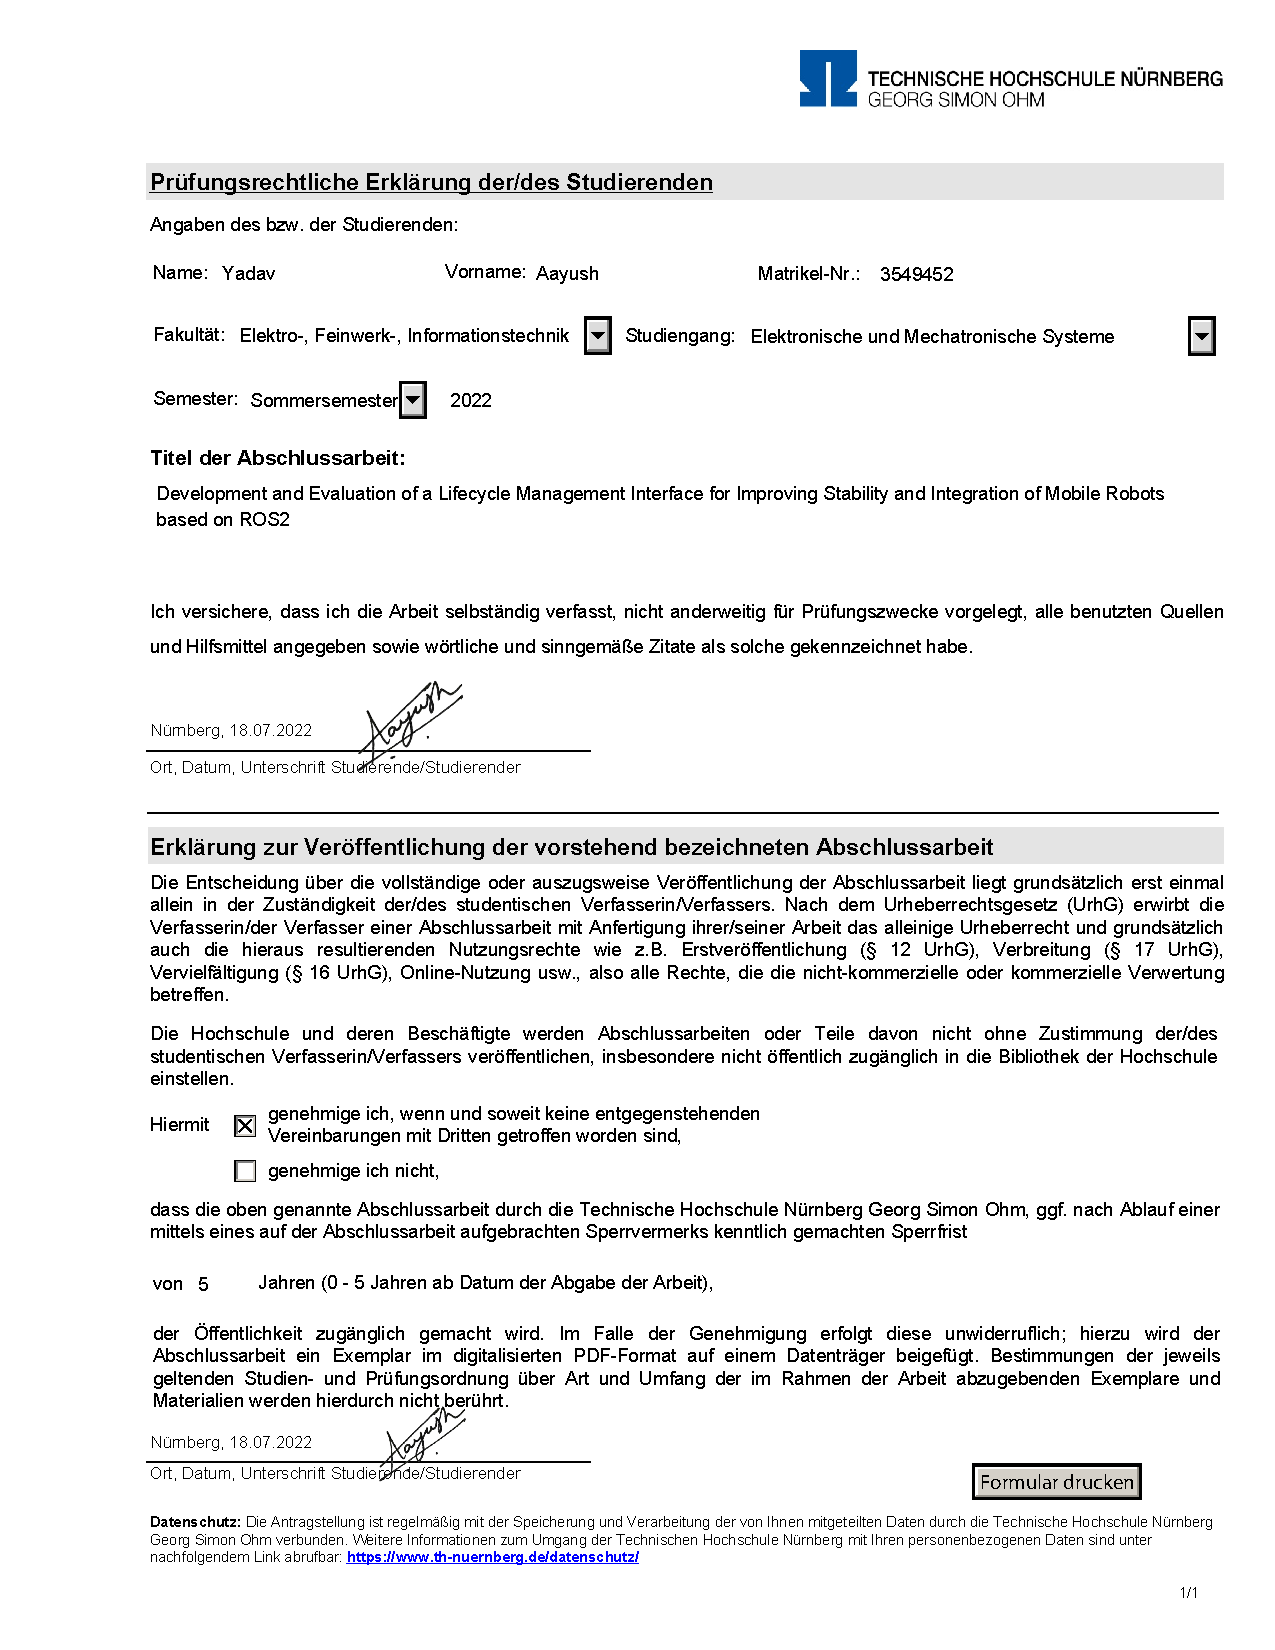
\includepdf[pages={1}]{Erklaerung_zur_Veroeffentlichung.pdf} %Erklärung zur veröffentlichung
	
% \chapter*{Sperrvermerk}
% \label{Sperrvermerk}
% Die vorliegende Arbeit \glqq \textbf{Eine Methode zur Evaluierung und Implementierung eines Datenbankkonzeptes zur Prozessoptimierung einer SW-Testdatenauswertung}\grqq\ beinhaltet interne vertrauliche Informationen der AKKA DSO Ingolstadt GmbH. Die Weitergabe des Inhalts der Arbeit im Gesamten oder in Teilen sowie das Anfertigen von Kopien oder Abschriften -- auch in digitaler Form -- sind grundsätzlich untersagt. Ausnahmen bedürfen der schriftlichen Genehmigung der AKKA DSO Ingolstadt GmbH.
% \addcontentsline{toc}{chapter}{Sperrvermerk}

\chapter*{Eidesstattliche Erklärung}
\label{erklaerung}

Hiermit versichere ich, die vorliegende Abschlussarbeit selbstständig und nur unter Verwendung der von mir angegebenen Quellen und Hilfsmittel verfasst zu haben. Sowohl inhaltlich als auch wörtlich entnommene Inhalte wurden als solche kenntlich gemacht. Die Arbeit hat in dieser oder vergleichbarer Form noch keinem anderem Prüfungsgremium vorgelegen. \\
\\[1.5cm]
Datum:	\hrulefill\enspace Unterschrift: \hrulefill
\\[3.5cm]
% \addcontentsline{toc}{chapter}{Eidesstattliche Eklärung}

% \chapter*{Danksagung}
% \label{Danksagung}
% Danke an alle

% % \addcontentsline{toc}{chapter}{Danksagung}

% \chapter*{Zusammenfassung}
% \label{Zusammenfassung}
% Die AKKA DSO Ingolstadt GmbH beschäftigt sich mit der Entwicklung und Erprobung von Software für verschiedene Fahrzeugsteuergeräte, Fahrzeugfunktionen und Fahrerassistenzsysteme. Dazu werden HiL-Simulatoren (Hardware in the Loop) eingesetzt. Im Labor werden Teile des Fahrzeugs oder gegebenenfalls das gesamte Fahrzeug so simuliert, dass ein Fahrzeugsteuergerät und andere Fahrzeugfunktionen unter verschiedenen Betriebssituationen getestet werden können. Dies ermöglicht die Automatisierung von Fahrzeugtests und beschleunigt den gesamten Entwicklungsprozess. Während des Testprozesses entstehen riesige Datenvolumen, die für die Analyse der einzelnen Tests und für die Verfolgung des Entwicklungsfortschritts notwendig sind. Es scheint ein Bedarf für eine Anwendung mit zentraler Datenbank zu bestehen, die einen einfachen Zugriff auf die Test-Daten ermöglicht und den Verlauf des Entwicklungsprozesses leichter nachvollziehbar macht. Diese Anwendung muss in der gesamten Abteilung von allen beteiligten Mitgliedern benutzbar sein. Diese Bachelorarbeit beschreibt die Konzipierung und eine Methode zur prototypischen Entwicklung dieses Testdatenauswertungswerkzeugs.

% Der Schwerpunkt dieser Arbeit liegt allerdings auf dem Entwurf und der Implementierung eines webbasierten Datenverwaltungsystems. Die verwendete Softwarearchitektur, der Entwicklungsprozess einer Webanwendung, die eingesetzten Frameworks und das zugrundeliegende Datenbanksystem werden im Detail beschrieben. Die zum Verständnis einer Webanwendung notwendigen Grundlagen werden im Kapitel \ref{sec:grundlagen} erläutert. In der Entwurfsphase werden die Anforderungen an das System ermittelt und das Anwendungskonzept unter Berücksichtigung der erarbeiteten Anforderungen erstellt. Für die Implementierung der Webanwendung werden die Programmiersprachen Python und Javascript verwendet.

% \addcontentsline{toc}{chapter}{Zusammenfassung}

% \chapter*{Abstract}
% \label{Abstract}
% AKKA DSO Ingolstadt GmbH is engaged in the development and test of software for various vehicle control units, vehicle functions and driver assistance systems. HiL simulators are used for this purpose. In the laboratory, parts of the vehicle or, if necessary, the entire vehicle is simulated in such a way that a vehicle control unit and other vehicle functions can be tested under various operating situations. This enables the automation of vehicle tests and accelerates the entire development process. During the test process, large volumes of data are generated, which are necessary for the analysis of the individual tests and for tracking the progress of the development. There seems to be a need for an application with a central database, which allows easy access to the test data and makes it easier to track the progress of the development process. This application must be usable throughout the department by all involved members. This bachelor thesis describes the conception and a method for the prototypical development of this test data evaluation tool.

% However, the focus of this work is on the design and implementation of a web-based data management system. The chosen software architecture, development process of a web application, used frameworks and underlying database system are described in detail. The basics necessary for understanding a web application are explained in the chapter \ref{sec:grundlagen}. In the design phase, the requirements for the system are determined and the application concept is developed taking the determined requirements into consideration. The programming languages Python and Javascript are used to implement the web application.

% \addcontentsline{toc}{chapter}{Abstract}
	% Hier Römische Seitenzahlen auch angeben
	\ofoot{\pagemark}
	
	% Abstract
	% Inhaltsverzeichnis
 	\tableofcontents
	
	% Glossar
	% Alle Einträge ausgeben
	\glsaddall
	% Glossar darstellen
	% \printglossary
	% \label{sec:Glossar}
	
	% Abkürzungsverzeichnis
	% \printglossary[type=\acronymtype, title=List of Acronyms, style=mylong]
	% \printglossary
	% \printglossaries

	\printnoidxglossary[type=\acronymtype,title=List of Acronyms, style=mylong]

	% Aufräumen und Seitenanzahl speichern
   	\clearpage
   	\setcounter{SeitenzahlSpeicher}{\value{page}}
   	\label{Ende_Vorgeplaenkel}
   	
	% Inhalt
	% Hier wieder umstellen auf arabisches Seitenzählen
	\pagenumbering{arabic}
	\ofoot*{{\pagemark} of \pageref{Ende}}
	
	\chapter{Introduction}
\label{Introduction}

	\section{Motivation}
	\label{Introduction:Motivation}
	Modern robotic Systems are made up of several individual and independent components. As systems grow in size and become more complex and sophisticated it becomes more and more difficult to have a proper overview of the complete system and at the same time the troubleshooting, debugging and streamlined operation becomes more challenging. To solve this problem there is a need for a solution that helps to improve the overall system satability and facilitates system Integration. In this thesis a ros2 system with managed lifecycle nodes which run inside a docker enviroment and a management interface for these lifecycle nodes is developed. Furthermore the docker based appliation is converted to a Siemens Industrial Edge Application which helps to streamline the delivery and deployment of the developed application within the Siemens industrial edge infrastructure.
	
	\section{Problem Statement}
	\label{Introduction:Problem Statement}
	In a current ROS2 based robotic system (AGV) there are several subsystems running simultaneously in order to operate seamlessly. If any of these independent systems fail the whole system fails and a developer must work on the AGV to troubleshoot and fix the problem. This entire processs is very tedious, time consuming and not efficient. If these problems could be debugged and solved from a remote (web) Interface, that would offer huge benifits to the overall system. So each individual systems will be packaged as a ROS2 lifecycle nodes with custom lifecycle behaviours, which would allow a user to dynamically reconfigure individual nodes, restart or respawm the nodes remotely and get the debug and other operationl information throug a remote logger.

	Another problem is the delivery and deployment, currently all the installation process needs to be done manually, i.e a developer has to login to a specific AGV install each library and dependencies necessary for a specific application. This process can be streamlined and made way more efficient by introducing a docker based appliation that can be installed using the Siemens industrial edge infrastructure. Another major task of this thesis is to utilize the DDS offerd by ROS2 and operate a Lifecycle managment Interface within a Local network. This amplyfies the efficiency of the system drasticly and offers new offortunities to control a swarm of robots through a single unified Web-interface.
	
	\section{Requirements}
	According to \cite{Koubaa2021}, the following questions must be answerable after the analysis phase of the software development process:
	\begin{itemize}
		\item What are the crucial requirements for the software to be created?
		\item What problem is to be solved with the help of the application system?
		\item What do your customers and users want from the system?
		\item Development enviroment
		\item Restrictions / Bounding conditions
		\item Minimum vaible Product
		\item 
	\end{itemize}
	
	
	% \chapter{Stand der Technik}
\label{StandDerTechnik}
	\section{Bestehende Systeme}
	\label{StandDerTechnik:Sub1}
	
	\section{Zusammenführen von Programmen jetzt}
	\label{StandDerTechnik:Sub2}
	Diese Masterarbeit 
	Das System \cite{Laura}
	
	\chapter{Background}
\label{Background}

This chapter gives an outline of the concepts and a detailed explanation of the various technologies that will be used later in this thesis.

	\section{Containers}
	\label{Background:Containers}
	The concept of container technology uses the same model as shipping containers in transportation. The idea is that before the invention of shipping containers, manufacturers had to ship goods in a variety of fashions which included ships, trains, airplanes, or trucks, all with different sized containers and packaging.
	With the standardization of shipping containers, products could be transported seamlessly without further preparation using different shipping methods. Before the arrival of this standard, shipping anything in volume was a complex, laborious process. The motivation behind software containers is the same. \cite[P.~1]{Kinnary2018}\\

	Instead of shipping a complete operating system (OS) and the software (with necessary dependencies), we pack our code and dependencies into an image that can run anywhere. Furthermore,  it enables the packaging of clusters of containers onto a single computer. In other words, a container consists of an entire runtime environment: an application, plus all the dependencies, libraries, and other binaries, and configuration files needed to run it, bundled into one package.
	The ability to have software code packaged in pre-built software containers means that code can be pushed to run on servers running different Linux kernels or be connected to run a distributed app in the cloud. This approach also has the advantage of speeding up the testing process and creating large, scalable cloud applications. This approach has been in software development communities for several years. It has recently gained in popularity with the growth of Linux and cloud computing. \cite[P.~2]{Kinnary2018}\\
	
	% \newpage
	\subsection{Containerization vs Virtualization}
	Linux containers and virtual machines (VMs) are both package-based computing environments that combine several IT system components and keep them isolated from the rest of the system. Their main distinguishing features are scalability and portability. Containers are usually measured in megabytes, whereas VMs in gigabytes.
	\cite{containersRedHat}
	\begin{figure}[H]
		\centering
		% \input{"Bilder/tikz/Grundlagen/docker-types-of-mounts.tex"}
		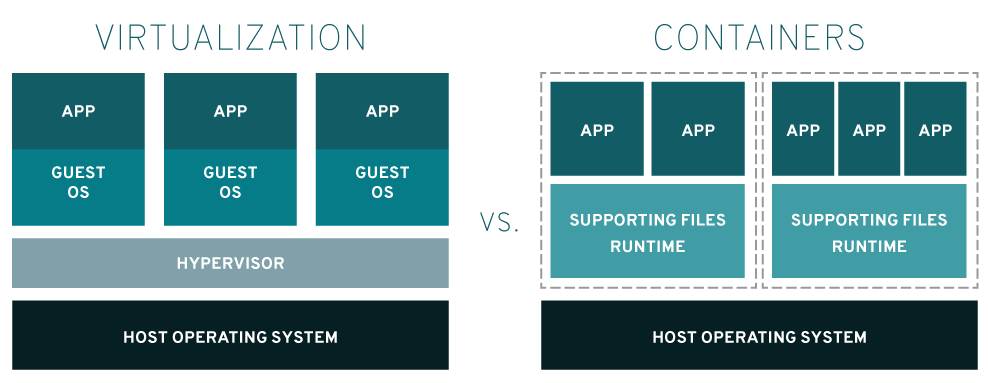
\includegraphics[width=0.9\textwidth]{"Bilder/virtualization-vs-containers_transparent.png"}
		\caption{Differences between Virtualization and Containerization \cite{containersRedHat}}
		\label{fig:Background:Containers:Containers vs VMs}					
	\end{figure}

	\paragraph*{Containerization} is an alternative to standard virtualization that encapsulates an application in a container with its executing environment.
	Containers hold an application and everything it needs to run. Everything within a container is maintained on an image—a code-based file that includes all libraries and dependencies. These files are similar to a Linux distribution installation. An image comes with RPM packages and configuration files. Containers are so small compared to VMs, there are usually hundreds of them loosely coupled together.\cite{containersRedHat}
	
	\paragraph*{Virtualization} is a way of sharing a single physical instance of a resource or an application to multiple organizations and clients. It utilizes software called a hypervisor that separates resources from their physical devices. It enables the partitioning of the resources and assigned to individual VMs. When a user issues a VM instruction that requires additional resources from the physical environment, the hypervisor sends the request to the physical system and saves the changes. VMs look and act like physical servers, which can multiply the drawbacks of application dependencies and large OS footprints—a footprint that's often not required to run a single app or microservice.\cite{containersRedHat} \\

	Table \ref{tab:container_vs_vms} illustrates the key differences between the above two approaches concerning package-based computing environments.
	\begin{table}[H]
        \centering
		\rowcolors{1}{}{gray!25}
        \begin{tabular}{{p{3cm}|p{5cm}|p{6cm}}}
            \toprule
            Parameters & Virtualization & Containerization\\
            \midrule
            Isolation & Provides complete isolation from the host operating system and the other VMs & Provides lightweight isolation from the host and other containers, but doesn’t provide a strict security boundary as a VM \\
            Operating System & Runs a complete operating system including the kernel, thus requiring more system resources such as CPU, memory, and storage & Runs the user-mode portion of an operating system, and can be customized to include just the required services for your app utilizing fewer system resources \\
            Compatibility & Runs just about any operating system inside the virtual machine & Runs on the same operating system version as the host\\
            Deployment  & Deploys individual VMs by using Hypervisor & Deploys single container by using Docker or deploy multiple containers by using an orchestrator such as Kubernetes\\
            Persistent storage  & Uses a Virtual Hard Disk (VHD) for local storage for a single VM or a Server Message Block (SMB) file share for storage shared by multiple servers & Uses local disks for local storage for a single node or SMB for storage shared by multiple nodes or servers\\
            Networking  & Uses virtual network adapters & Uses an isolated view of a virtual network adapter. Thus, providing a little less virtualization\\
            Startup time & They take few minutes to boot up & They can boot up in few seconds \\
            \bottomrule
        \end{tabular}
		\caption{Differences between Virtualization and Containerization \cite{containers-vs-vms-Baeldung}}
		\label{tab:container_vs_vms}
    \end{table}

	The use of containers can decrease the required time for developing, testing, and deploying applications. It makes testing and fault detection less complex as there is no difference between running your application on a test environment and in production. It provides a cost-effective solution and can help reduce operational and development expenses. In most use-cases, container-based virtualization offers several advantages over traditional Virtual Machine based virtualization.

	\section{Docker}
	\label{Grundlagen:Docker}
	\textit{Docker is a person who works at a port whose job is to load goods onto and off container ships.} \cite{docker-definition-english}

	Software Docker essentially does the same in the software context. Docker is a collection of open-source tools that quickly wraps up any application and all its unique dependencies in a lightweight, portable, self-sufficient container that can run virtually anywhere on any infrastructure.\cite{docker-definition}
	Docker was launched as an open-source project by dotCloud, Inc. in
	2013. it relies heavily on namespaces and cgroups to provide resource isolation and to package an application along with its dependencies. This bundling of dependencies into one package allows an application to run across different platforms and still support a level of portability. This provides flexibility to developers to develop in the desired language and platform. It has drawn a lot of interest in recent years.\cite[P.~10]{Kinnary2018}

	Docker consists of several parts. The following section gives an overview of the main components of Docker.


		\subsection{The Docker Runtime and Orchestration Engine (Docker Engine)} 
		\label{Grundlagen:Docker:Docker Engine}
		The Docker engine is the software for the infrastructure that runs and orchestrates containers. All other Docker, Inc. and third-party products connect to and develop around the Docker Engine. It provides a workflow for building and managing the application stack. It builds and runs containers using other Docker components and services. It consists of the Docker daemon; a REST API that specifies the interfaces that programs can use to communicate with the daemon; and the CLI, the command-line interface that communicates with the Docker daemon via the API. Docker Engine creates and runs the Docker container from the Docker image file.\\
		\\
		Following Diagramm illustrates the Docker System Architecture.
		\begin{figure}[H]
			\centering
			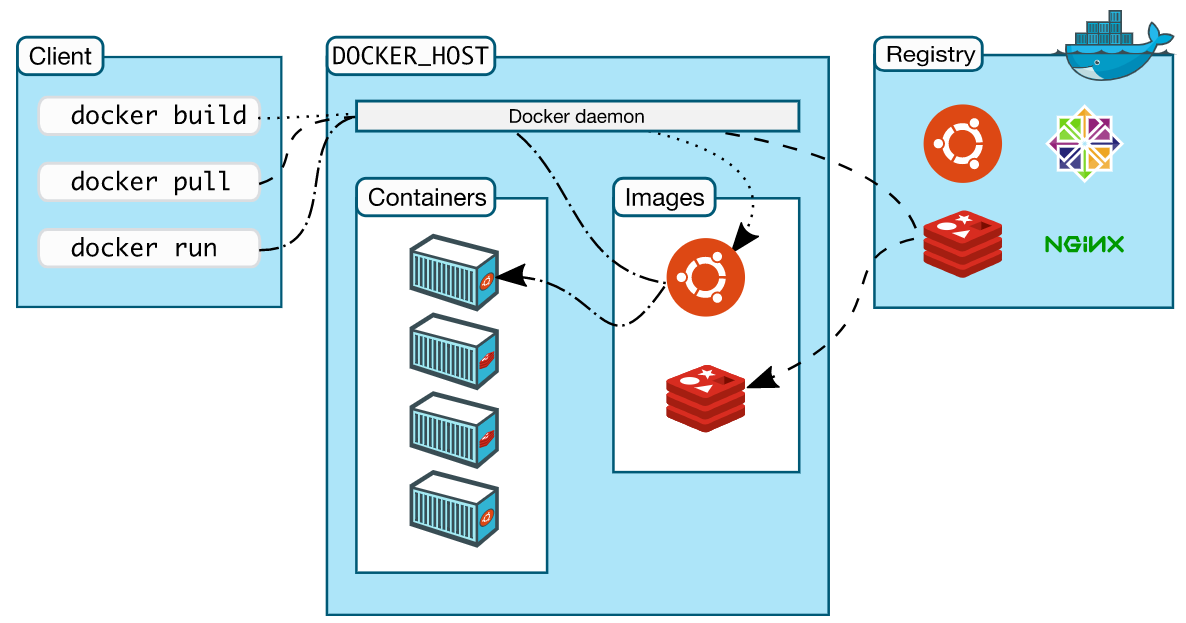
\includegraphics[width=0.9\textwidth]{"Bilder/DockerArchitecture.png"}
			\caption{Docker System Architecture \cite{dockerOverwiew}}
			\label{fig:Background:DockerEngine:Architecture}					
		\end{figure}

		\paragraph{Docker daemon (dockerd)}  is a server process that runs
		in the background. It continuously listens to the REST API interface
		and listens for incoming requests and manages Docker objects (images, containers, networks, and volumes).  A daemon also has the ability to communicate with other daemons to manage Docker services.\cite{dockerOverwiew}

		\paragraph{Docker client} represents the primary means for most users to interface with Docker. The commands run through the command-line interface are sent to the Docker daemon through the Docker API interface. The Docker daemon(dockerd) then executes these commands. The Docker client has the ability to connect with multiple Docker daemons.\cite[P.~32]{Kinnary2018}
		
		\paragraph{Docker registry} The images created by the Docker daemon are stored in the Docker registry. Docker looks for images in the Docker Hub by default, but it is possible to have a self hosted private registry. Docker Hub is a public registry and is freely accessible.\cite[P.~33]{Kinnary2018}
			
		\subsection{Docker Objects}
		\label{Grundlagen:Docker:Docker Objects}
		\paragraph{Images}
		A Docker image is a read-only file system that contains instructions to create a container in which an application can run. In most cases, a Docker Image is based on another image and is customized. You can either use existing images published in public repositories such as Docker Hub or Create your image.
		A Dockerfile is used to create a Docker image. A Dockerfile contains simple instructions that can be understood by the Docker daemon to	create the image and run it. Docker images are layers that correspond to each instruction in the Dockerfile. Part of what makes a Docker image super easy is that when you change a part of the Dockerfile, only that layer is changed, and not the entire image.

		\paragraph{Containers}
		A Docker container is an instance of an image. An image runs inside a container. You can manage a container with the stop, start, and delete commands to manage it. Multiple containers can be connected over a network. They can be connected to the memory, and they can also communicate with each other. Containers are much more lightweight than VMs because their startup times are very fast. To create a container, in addition to the container's configuration and settings, you also create an image Configuration and settings an image is created. When a container is deleted everything related to the container is also deleted, including state and memory.

		\paragraph{Services}
		In a distributed application, different functionalities of the app provide different services. For example, if you are building an application that suggestions based on keywords that the user enters, you might want to have A front-end service that takes the word and sends it to the service that will Verifies the legitimacy of the word. This in turn could be sent to another service that runs an algorithm to generate the suggestions, etc., which are then returned to the service. These are all different services on different Docker containers, sitting Sit behind different Docker daemons. These Docker daemons are all connected over the network and interact with each other.
		All these services work together as a swarm, managed by different Managers and workers to manage. Each swarm contains a Docker daemon. These Daemons communicate with each other using the Docker API. A Docker Compose YAML file is used to get all these services running together. together to get them running. 

		\paragraph{Networks}
		One of the reasons Docker containers and services are so substantial is the ability to interconnect them or connect them to non-Docker workloads. Docker containers and services, in general, don't even need to be aware of the fact that they are deployed on Docker, or whether or not their peers are also Docker workloads. Whether the Docker hosts are running on Linux, Windows, or a mix of both, Docker can be used to manage them in a platform-independent way. Docker's network subsystem is extensible using drivers. By default, several drivers provide basic networking functions.\cite{dockerNetwork} 
		Within the Networks option of a Docker-compose file,  a network to which each service wants to connect can be specified. In addition, a default network to be used for the entire application can be specified. If there is an existing network that the containers should join, this is an option to use the external network.\cite{Kinnary2018}
		
		\paragraph{Volumes}
		Volumes are the preferred storage mechanism for data created and used by Docker containers. Volumes are fully managed by Docker and are independent of the host's directory structure and operating system. Volumes are easier to back up or migrate. They can be managed with Docker CLI commands or the Docker API. Volumes can be safely shared between multiple containers. For new volumes, the content can be pre-populated by a container. In addition, volumes are often a better choice than storing data in a container's writable layer because a volume does not increase the size of the containers that use it, and the contents of the volume exist outside the lifecycle of a particular container. In the Volumes option of a Docker Compose file, the volumes to be mapped from the host machine to the Docker container can be specified for each service.\cite{dockerStorage}
			
		\subsection{Dockerfiles}
		\label{Grundlagen:Docker:Dockerfiles}	
		Dockerfile is a text document that contains a set of instructions or commands for assembling an image that is understood by the build engine. The Dockerfile defines what goes into the environment inside your container. Accessing resources, mapping volumes, passing arguments, copying files that need to be inside your container are defined in this file. According to Dockerfile created, you need to build it to create the image of the container. Create container image. The image is just a snapshot of all the executed statements in the Dockerfile. Once this application image is created, you can expect that it will run on any machine that uses the same kernel. 
		
		\subsection{Docker-Compose}
		\label{Grundlagen:Docker:Docker-Compose}	
		Docker Compose is the tool for running multi-container Docker applications. It is essentially a YAML file that can be thought of as a Compose of multiple Dockerfile containers, which can be used to put commands into a single file. This Docker Compose YAML file contains configurations of multiple services. Then, with a single command, you can run all services to run in Docker containers at the same time.
		Docker Compose can be used to create a microservices architecture and link the containers together, or it can be used for a single service. In addition, Docker Compose can create images, scale containers, and re-run containers that have been stopped. All of these functions are part of Docker. Docker-compose is just a higher-level abstraction of container execution commands. Everything that a compose file can do, can likewise be performed with simple Docker commands, except that this requires more memory and additional overhead to execute any additional commands, to connect to the network, etc. . Docker-compose helps to simplify this process.
				
	\section{Industrial Edge}
	\label{Grundlagen:IndustrialEdge}
		
	Industrial Edge is a development from Siemens that makes it possible to analyze data generated in various industrial processes on the device itself. It combines local engineering with cloud engineering.\cite{siemensIndustrialEdge}

	This eliminates unnecessary data transport between the end device and the server, only processed data is sent to the server. The processing load is in this way directed from the server towards the end device. Edge applications serve this purpose, they contain a fixed set of functions and can be accessed with the edge infrastructure on the respective end device (edge device). These apps are based on Docker technology and run one or more Docker containers in them. Figure \ref{fig:Grundlagen:IndustrialEdge:Ueberblick} shows a typical infrastructure from the top server to the end devices.

		\begin{figure}[h]
			\centering
			%\input{"Bilder/tikz/Grundlagen/industrial-edge-overwiev.tex"}
			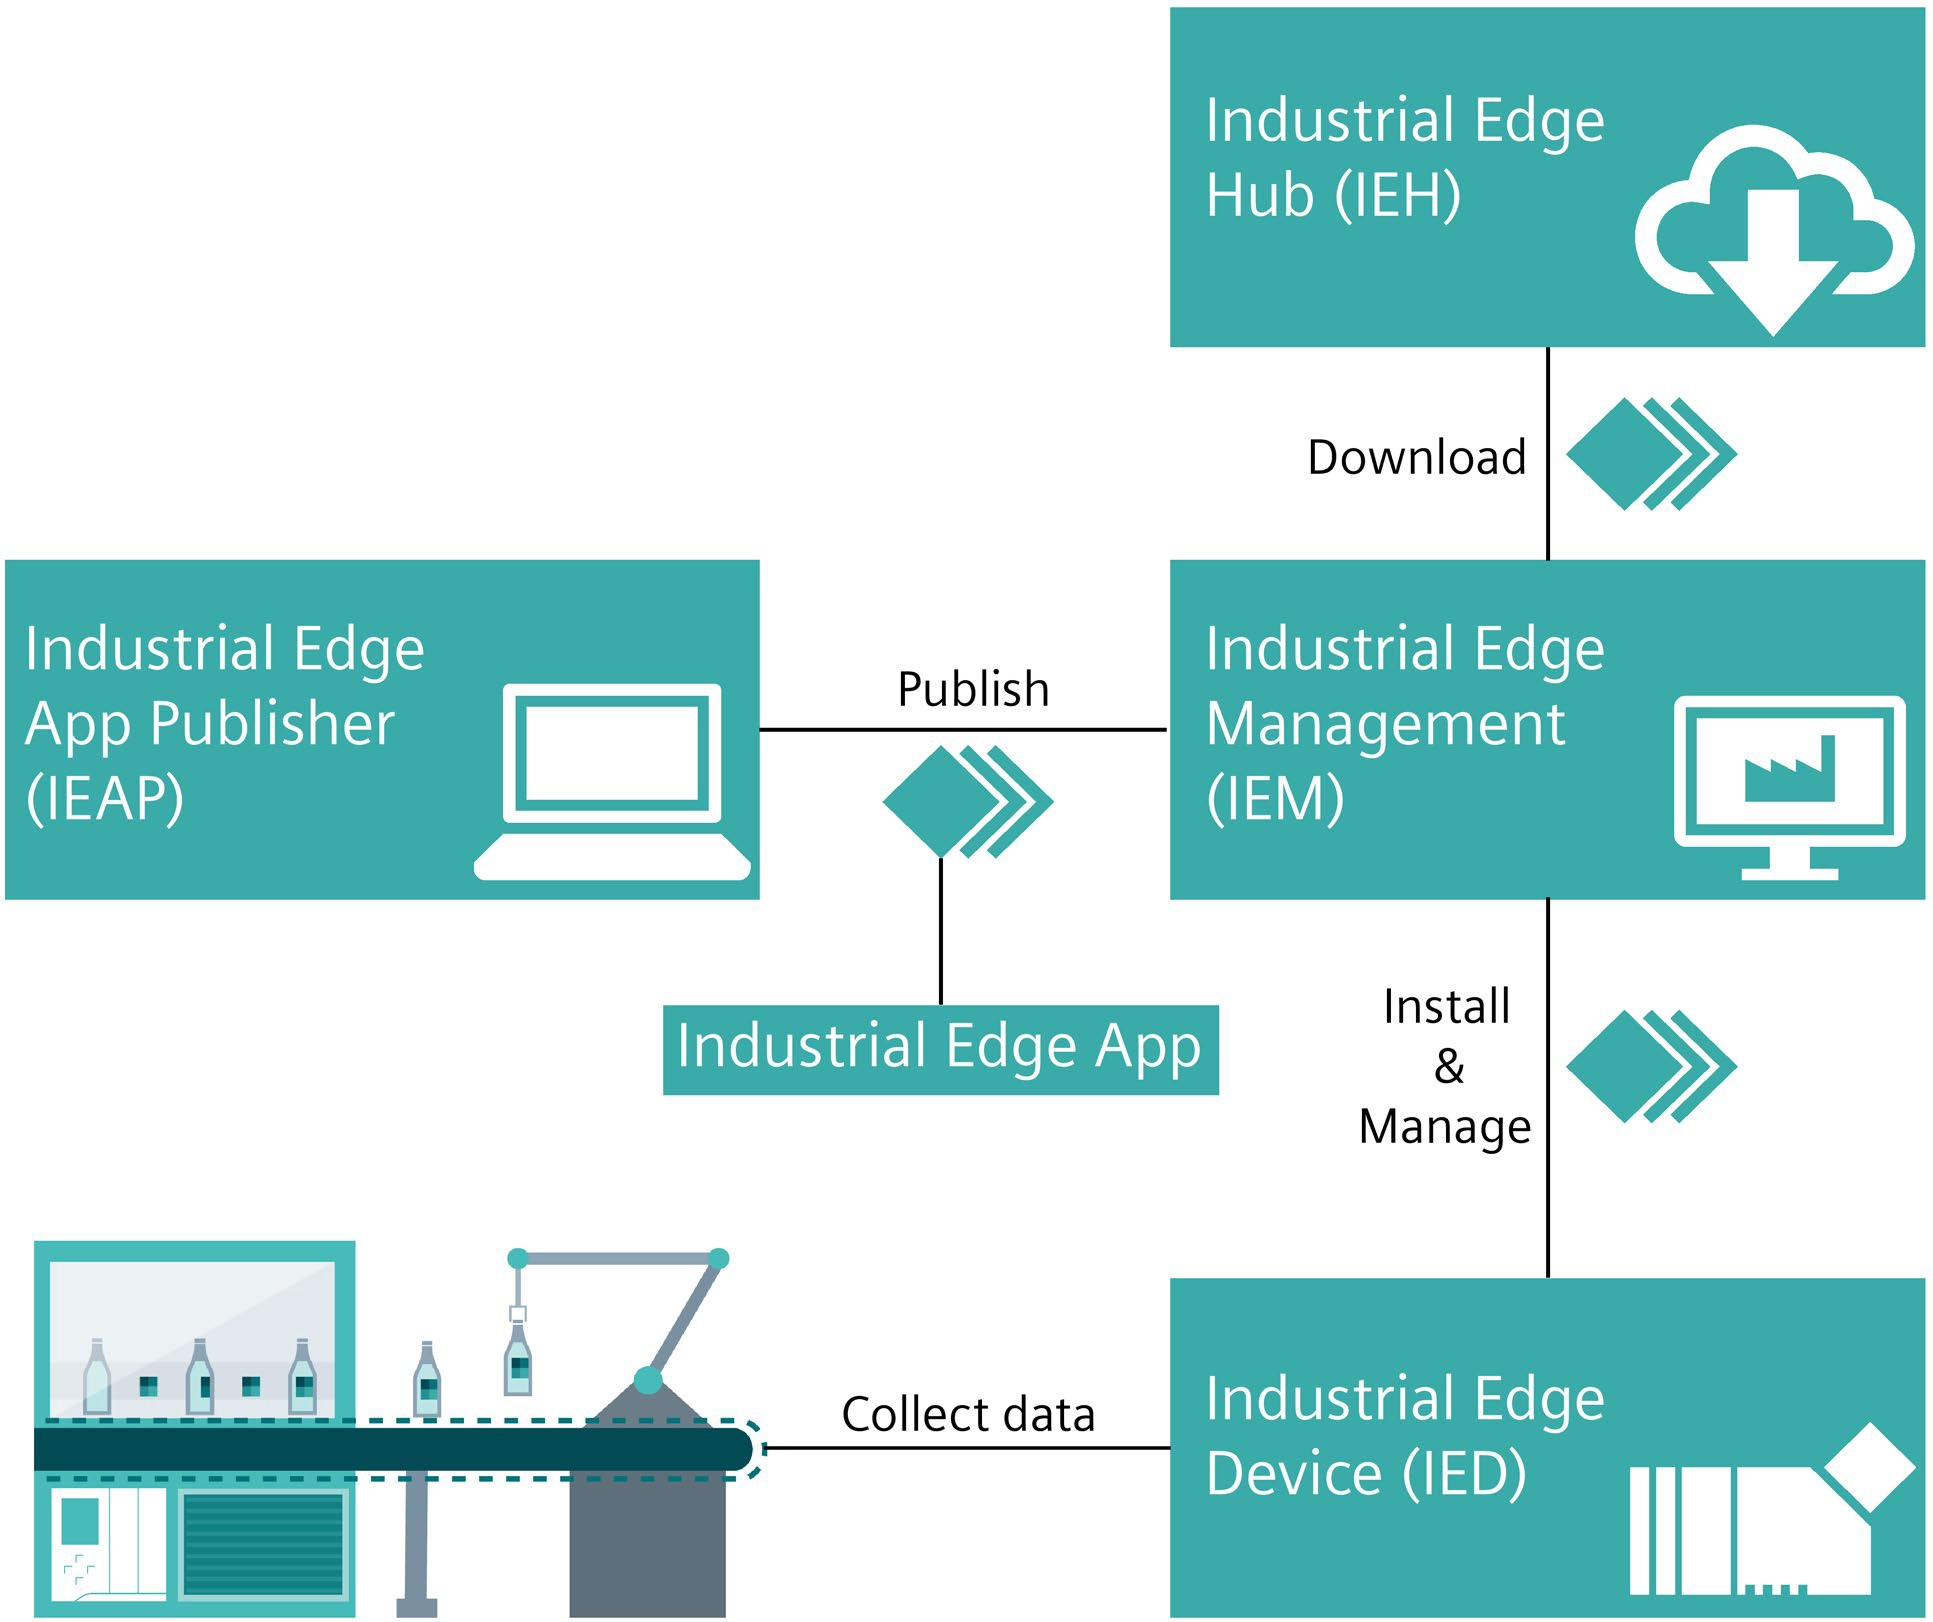
\includegraphics[width=0.70\textwidth]{"Bilder/Edge_uebersicht.jpg"}
			\caption{Industrial Edge overview \cite{siemensIEM_gettingStarted}}
			\label{fig:Grundlagen:IndustrialEdge:Ueberblick}					
		\end{figure}
	
		%- Management tool für Docker Container auf Geräten (Device)\\
		%- Graphen die das IE-Hub, IEM, Docker Device erklärt\\
			
		\paragraph{Industrial Edge Management System}
			The \gls{IEM} is a server, which can be operated independently in a local network. It allows the user to create their own server which avoids the transmission of raw sensitive data exchanged between the edge device and the IEM over the Internet.

			In addition, the end(edge) devices can be managed via this server, which includes the installation of apps and software updates and further analysis of individual apps. A self-developed Application can be uploaded to the IEM, which in turn can distribute it to the edge devices.\cite{siemensIndustrialEdge}

		\paragraph{Industrial Edge Hub}
			The \gls{IEH} 
			is the top server-level Application hub provided by Siemens. On this platform, Siemens offers applications developed in-house. These can be loaded onto the IEM for a license fee. Any required software packages and documentation can be downloaded from here. This streamlines the development process of custom applications including deployment, and operation on desired IEM.\cite{siemensIndustrialEdge}
		\paragraph{Industrial Edge App}
			An \gls{IEA} (edge app) is used for the intelligent processing of industrial automation tasks.\cite{siemensIndustrialEdge} It is a Docker-based image, which is runs on the IED. A docker-compose file acts as the top description level file, it specifies various parameters and the sequence in which the Docker images are started. The parameters include network configuration, data storage, and other application-specific configurations. It supports all Docker-compose version 2.4 settings. Modification of this docker-compose file allows configuring any Edge app, even after it has been already downloaded to an edge device. An Edge App can be downloaded to an edge device through the IEM.
	
		\paragraph{Edge Device}
		Edge devices are required in order to run individual edge apps. The edge device is a custom Linux Machine running the Industrial Edge OS. For test and simulation purposes it can also be run in a Virtual machine(VM). Edge devices can save automation data locally and retrieve it when required. In addition, edge devices can upload this data into the cloud infrastructure and retrieve it at any moment. After proper configuration and connection,  an Edge Device can be activated through IEM using an Edge Device configuration file.
			
		\paragraph{Industrial Edge Publisher}
		The Industrial Edge Publishers is a tool that converts Docker images into Edge Apps and uploads them to the IEM. It can also be used to manage, modify or delete apps that have already been created.\cite{siemensIE_App} A prerequisite for creating an app is a docker-compose file, which contains the startup parameters of a Docker container. These parameters can also be configured through a menu within the Edge Publisher.
			

	
	\section{ROS}
	\label{Grundlagen:ROS2}		
	This chapter covers the basics of the robot operating system (ROS) and all the tools necessary to create, debug, and understand robot applications. This chapter describes some high-level concepts and low-level API commands which enable developers to develop, maintain and support multi-robot applications. \\
	
	The software stack of a typical robot system requires several software tools which include hardware drivers, network modules, communication architecture, and several application-specific algorithms. ROS provides these tools in one package, which saves developers a lot of time and redundant work. ROS includes several sub-packages for robot navigation, vision, control, simulation.\\
	
	The Robot Operating System (ROS) has long been one of the most widely used middleware for robotic. The large open-source robotics community has contributed to a lot of new features since the introduction of ROS 1 in 2007, limitations of ROS1 have led to the development of ROS2.\cite{ros2Basic}\\

	\subsection{ROS2} 
	\label{Grundlagen:ROS:ROs2}
	\gls{ROS2} was launched with an improved architecture and upgraded features. It is new and various organizations and open-source communities are trying to port existing packages to ROS 2.\cite{ros2Basic} \\
	
	Table \ref{tab:ros1_vs_ros2} illustrates the key differences between ROS1 and ROS2
	\begin{table}[H]
        \centering
		\rowcolors{1}{}{gray!25}
        \begin{tabular}{{p{3cm}|p{5cm}|p{6cm}}}
            \toprule
            Parameters & ROS1 & ROS2\\
            \midrule
            Networking & Utilizes the TCPROS communication protocol & Uses DDS (Data Distribution System) for communication.\\
            ROS Master & Uses ROS Master for centralized discovery and registration. The whole communication system fails if the master fails. & Uses the distributed DDS discovery. ROS 2 provides a custom API to get all information about nodes and topics. \\
            Compatibility & ROS runs only in Ubuntu. & ROS 2 is compatible with Ubuntu, Windows 10, and OS X.\\
            Programming language  & Uses C++ 03 and Python2. & Uses C++ 11 and Python3.\\
            Build system  & ROS uses only the CMake build system and has a combined build for multiple packages via a single CMakeLists.txt file & ROS 2 offers options to use other build systems. Supports isolated independent builds for packages to better handle dependencies between packages.\\
            Default values & Data types in message files do not support default values. & Data types in message files support default values.\\
            roslaunch & roslaunch files are written in XML. & roslaunch files are written in Python which makes it more configurable and and supports conditional execution.\\
            Realtime Support & Does not support Real-time behavior. & Supports real-time responses with a suitable RTOS.\\
			\bottomrule
        \end{tabular}
		\caption{Differences between ROS1 and ROS2 \cite{ros1vsros2}}
		\label{tab:ros1_vs_ros2}
    \end{table}

	\subsection{ROS2 Structure}
	\label{Grundlagen:ROS2:ROS2_Structure}
	The key ROS2 feature is that it uses DDS (Data Distribution System) for communication. It eliminates ROS Master and utilizes distributed DDS discovery.	A set of related nodes located on the same computer are called a hub, where one or more hubs can be present on the same computer. ROS hubs are considered to have an accompanying set of bridging nodes that pass messages between ROS and ROS2.\cite*[P.7]{Koubaa2021}
	\begin{figure}[H]
		\centering
		% \input{"Bilder/tikz/Grundlagen/docker-types-of-mounts.tex"}
		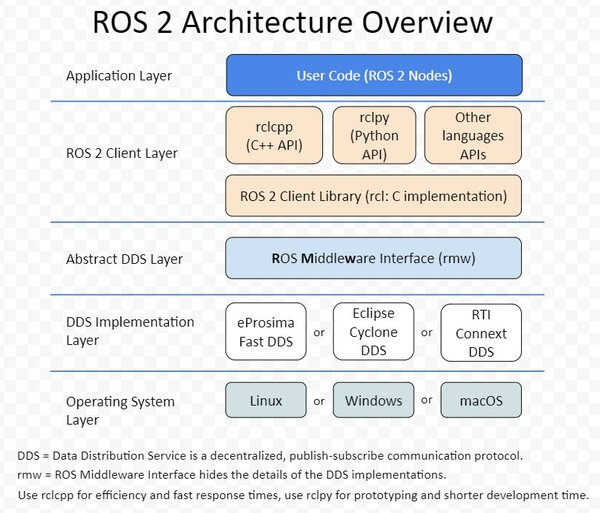
\includegraphics[width=0.8\textwidth]{"Bilder/ros-architecture.jpg"}
		\caption{ROS2 Architecture \cite{ros-2-architecture}}
		\label{fig:Background:Containers:Ros2_Architecture}					
	\end{figure}
	
	\subsection{ROS2 Nodes (Application layer)}
	\label{Grundlagen:ROS2:ROS2Nodes}

	In ROS distributed applications are typically designed as entities referred to as nodes. Each Node in ROS is supposed to be responsible for a single, modular function. In a Robotic Control System, sensors (lidar, camera), motion controllers (motors for movement), and algorithm components (route planners) can each be nodes.  A node can send and receive data to and from other nodes via topics, services, actions, or parameters.
	ROS 2 separates the node concept from the process structure at the operating system level. Multiple nodes can be created within a process as desired, and these nodes can independently interact with other nodes. All nodes in the system can run on a single computer or they can be distributed and run on multiple computers.


	\paragraph[ROS2]{ROS2 Communication Patterns}
	\label{Grundlagen:ROS2:CommunicationPatterns}

	The nodes communicate with each other via topics, service calls, and actions. Topic-based Communication is based on a publish-subscribe architecture, where the data generated and published by a node can be subscribed to by more than one node, and likewise, a Topic can produce data for more than one node. 
	The distributed architecture of the topic topology offers improvements in terms of performance and fault tolerance. Additionally, the extensive quality of service(QoS) features in the DDS middleware layer make ROS-2 architecture more robust and enable developers to use it in an industrial- /real-life application.

	A comprehensive robotic system has several nodes working together in harmony. In ROS 2 a single executable (C++ program, Python program, etc.) can hold one or more nodes in them. This network of ROS 2 elements running simultaneously and processing data is referred to as a ROS graph. It includes all executables and the connections between them.



	\begin{figure}[H]
		\centering
		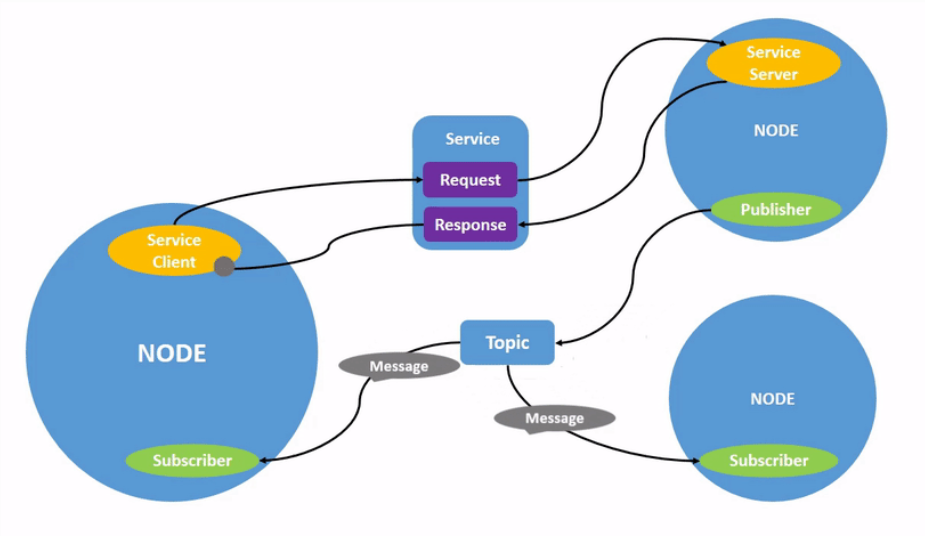
\includegraphics[width=0.8\textwidth]{"Bilder/ros-nodes.png"}
		\caption{ROS2 Communication Pattern \cite{ros2Basic}}
		\label{fig:Background:Ros2Nodes}					
	\end{figure}

	\begin{labeling}{Messages:}
		\item [Messages:] 
		A message is a data file that is sent via a communication channel called. Messages in ROS 2 are of great importance for interoperability. A publisher sends its message to a specific topic. This topic can be subscribed to by one or more subscribers. Several publishers can send messages to a topic and several subscribers can receive them. The communication in messages is unidirectional. A topic must use a message type that is known to all participants. There are predefined standard message types that are supplied with the ROS2 installation. Custom message types can be defined in a .msg- file. A message can contain other message definitions and can be extended using this pattern.\cite*{ros2Tutorials}
		
		\item [Topics:] 
		Topics act as virtual communication channels (bus) through which data is moved between nodes and consequently between various components of the system. Topics aren't just one-to-one connections moreover, they can be many-to-one, one-to-many, and many-to-many connections. Topics are a key element in realizing Publish-Subscribe architecture.
		Topics define the name and data structure used. Each topic in ROS2 is also an instance that can store historical message data in that topic.

		\item [Service:] 
		Two-way communication in ROS2 is made possible with services. A request is sent to a service server, which then responds to the request sent by the service client. A single service communication channel can contain several service clients but only one service server. The service server and service client must be both able to recognize the message type used. Custom service message types can be defined with a .srv file. This file defines the request and the response of service communication. A service can contain other service message definitions.
		\begin{figure}[H]
			\centering
			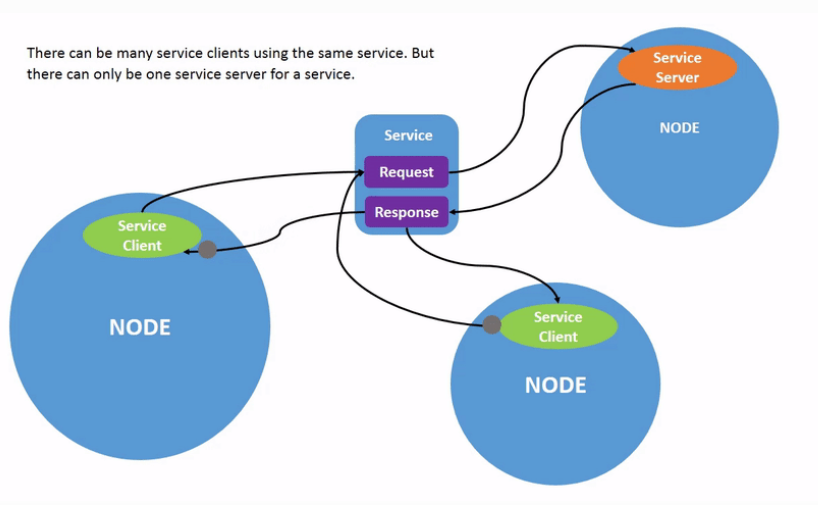
\includegraphics[width=0.8\textwidth]{"Bilder/ros-services.png"}
			\caption{ROS2 Services \cite{ros2Tutorials}}
			\label{fig:Background:Ros2Services}					
		\end{figure}
		
		\item [Action:]
		Actions are an advanced communication pattern in ROS2 that's designed for long-running tasks. They are made up of three parts: a goal, feedback, and result.
		Topics and services are the building blocks of Actions. Their functionality is similar to that of services, with the difference that actions are interruptible (they can be individually ended during execution). Unlike services, which only return a single response, they provide constant feedback.
		
		Actions use a client-server model, similar to the publisher-subscriber model. An "action client" node sends a goal to an "action server" node, which acknowledges the goal and returns a stream of feedback and a result. 

		\begin{figure}[H]
			\centering
			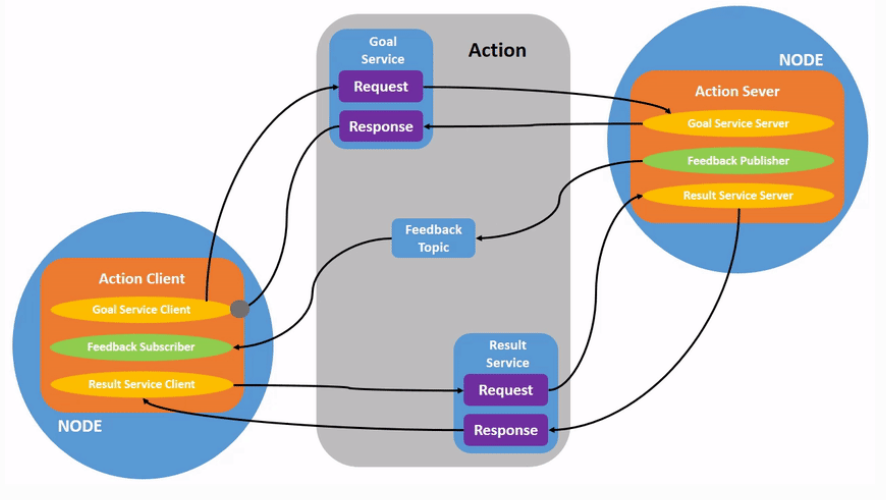
\includegraphics[width=0.8\textwidth]{"Bilder/ros-actions.png"}
			\caption{ROS2 Actions \cite{ros2Tutorials}}
			\label{fig:Background:Ros2Actions}					
		\end{figure}

		Figure \ref{fig:Background:Ros2Actions} gives an overview of the inner workings of an Action. The action client makes a Goal Request, which after processing can either be accepted or rejected by the action server. In case, the Goal Request is accepted it is forwarded to the action client. Then a user-defined function is called that executes the desired task of the action server. This Function continuously sends its current status or other custom information as feedback to the action client. Upon completion of the task and achievement of the defined goal, the action server sends the corresponding result response. Within an action communication channel, there can be several action clients, but only one action server. The action message type used must be recognized by all the participants in advance. Own action message types can be defined with a .action file. This contains the definition of Goal, Request, and Feedback. Other message definitions can be used from an existing action definition.		
		
	\end{labeling}

	\subsection{ROS2 Client Library}
	\label{Grundlagen:ROS2:ROS2ClientLibrary}
	Client libraries are the APIs that users can use to implement their ROS code. Client libraries give users access to ROS concepts such as nodes, themes, services, etc. Client libraries come in a variety of programming languages, so users can write ROS code in the language that best suits their application.

	Nodes written with different client libraries can exchange messages with each other because all client libraries implement code generators that allow users to interact with ROS interface files in the respective language.

	\subsection{ROS Middleware Interface}
	\label{Grundlagen:ROS2:ROSMiddlewareInterface}

	
	\subsection{Important ROS2 Concepts}
	\label{Grundlagen:ROS2:Concepts}

		
		The \text{ROS DOMAIN ID}\\
		About different ROS 2 DDS/RTPS vendors\\	
		About logging and logger configuration\\
		About ROS 2 client libraries\\
		About ROS 2 interfaces\\
		About parameters in ROS 2\\
		About topic statistics\\
		Introspection with command line tools\\
		About Composition\\
		On the mixing of ament and catkin (catment)\\

	\subsection{ROS2 Web Bridge}
	\label{Grundlagen:ROS2:2WebBridge}
		
	\subsection{roslibjs}
	\label{Grundlagen:ROS2:RosLibJS}
	
	

	\subsection{DDS}
	\label{Grundlagen:DDS}
		- Grundlage für Kommunikation von ROS2\\
		- Realisiert die eigentliche Kommunikation\\
		- Wenn das hier geht, geht auch ROS2!
		- Verschiedene Systemanbieter, näher wird RTI und Fastrtps untersucht: https://ros.org/reps/rep-2000.html  (Beide TIER 1)
		
	
	\section{Ros Lifecycle nodes}
	\label{Grundlagen:ROS2:Lifecycle}
	Having a managed lifecycle for nodes allows for better control over the state of the ROS system. This ensures that in a ROS2 Robotics System all components have been correctly instantiated before allowing a component to perform its behavior. It also allows nodes to be restarted or replaced online.

	A managed node has a known interface, executes according to a known lifecycle state machine. This allows the application (node) developer to decide how to implement various managed lifecycle functions while securing compatibility with other lifecycle nodes.\\
	
	The base functionality of a managed lifecycle node is described using a state machine illustrated in figure \ref*{fig:Background:Ros2LifecycleStateMachine}.\\

	\textit{"A state machine is a mathematical abstraction used to design algorithms. A state machine reads a set of inputs and changes to a different state based on those inputs. A state is a description of the status of a system waiting to execute a transition. A transition is a set of actions to execute when a condition is fulfilled or an event received."} \cite*{statemachineDef}\\

	There are 4 primary states (colored blue in figure \ref*{fig:Background:Ros2LifecycleStateMachine}):
	\begin{itemize}
		\item Unconfigured
		\item Inactive
		\item Active
		\item Finalized
	\end{itemize}
	In addition, there are 6 transition states, which are intermediate states during a requested transition(colored in yellow in figure \ref*{fig:Background:Ros2LifecycleStateMachine} ):
	\begin{itemize}
		\item Configuring
		\item CleaningUp
		\item Activating
		\item Deactivating
		\item ShuttingDown
		\item ErrorProcessing
	\end{itemize}
	There are 7 transitions exposed to the lifecycle management interface, which can be invoked only when the necessary conditions are met. These conditions are described in detail in the next section. The table below lists these transitions with the corresponding behavior invoked during their execution.
	\begin{table}[H]
		\centering
		\rowcolors{1}{}{gray!25}
		\caption{Availabe Transitions}
		\label{tab:Valid transitions}
		\begin{tabular}{|p{2cm}|p{9cm}|}
			\toprule
			Transition & Description\\
			\midrule
			create & with this transition the node is instantiated, but will not run any code beyond the constructor. On successful execution of the constructor the node is in Unconfigured state. \\
			configure & \textit{onConfigure()} callback is called\\
			cleanup & \textit{onCleanup()} callback is called\\
			activate & \textit{onActivate()} callback is called\\
			deactivate & \textit{onDeactivate()} callback is called\\
			shutdown & \textit{onShutdown()} callback is called\\
			destroy & with this transition the node is destroyed (deallocated). The node is completely removed from the system. \\
			\bottomrule
		\end{tabular}
	\end{table}

	\begin{figure}[H]
		\centering
		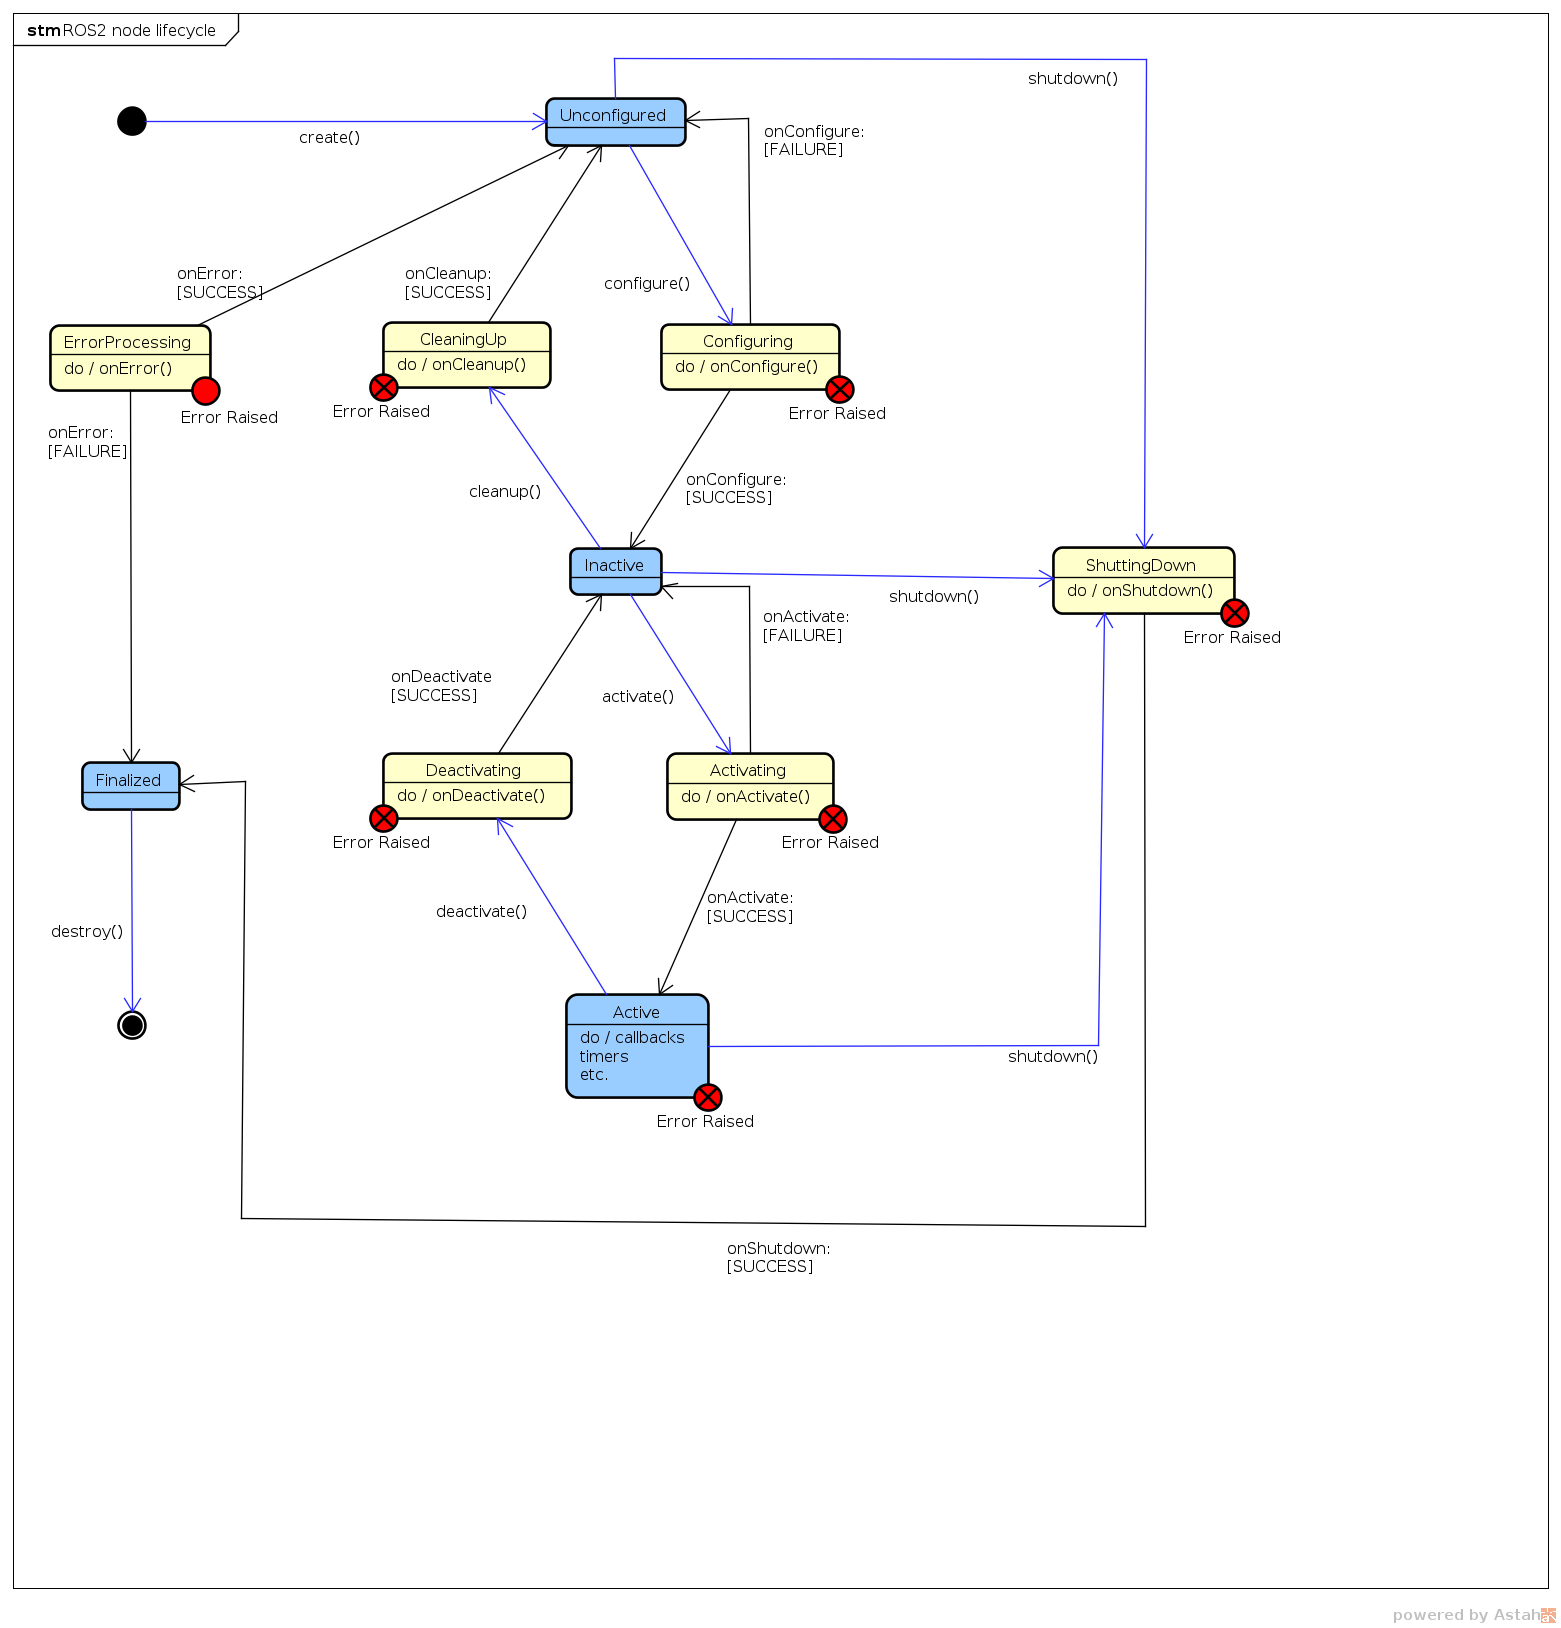
\includegraphics[width=0.95\textwidth]{"Bilder/ros_lifecycle.png"}
		\caption{ROS2 Lifecycle Statemachine \cite{ros-2-lifecycle}}
		\label{fig:Background:Ros2LifecycleStateMachine}					
	\end{figure}

	\subsection{Primary States}	
	The transition from a primary state requires an action of an external monitoring process, except in the case of an error triggered in the 3rd primary ("active") state.
	\begin{labeling}{Unconfigured:::::}
		\item[\textbf{Unconfigured}] This is the starting state of the state machine. When a node is instantiated, it finds itself in this lifecycle state. In case of any unexpected error, a node can be returned to this state. In this state, it is expected that there is no saved state. From this state the following transitions via corresponding transition states are availabe:
		\begin{table}[H]
			\centering
			% \rowcolors{1}{}{gray!25}
			\label{tab:Valid transitions}
			\begin{tabular}{|p{3cm}|p{3cm}|}
				\toprule
				Transition via & Final state\\
				\midrule
				configure & Inactive  \\
				shutdown & Finalized \\
				\bottomrule
			\end{tabular}
		\end{table}

		\item[\textbf{Inactive}] This state represents a node that is not currently operating. The main purpose of this state is to allow reconfiguration of a node (modifying configuration parameters, adding and removing topic publications/subscriptions, etc.) without changing its behavior during operation. In this state, the node does not read topics, process data, respond to functional service requests, etc. In the inactive state, all data arriving in managed topics is not read or processed. 
		
		Data storage is subject to the configured QoS policy for the topic. Any managed service requests to a node that is in the inactive state will not be answered (they will fail immediately for the caller). From this state the following transitions via corresponding transition states are availabe:
		\begin{table}[H]
			\centering
			% \rowcolors{1}{}{gray!25}
			\label{tab:Valid transitions}
			\begin{tabular}{|p{3cm}|p{3cm}|}
				\toprule
				Transition via & Final state\\
				\midrule
				shutdown & Finalized  \\
				cleanup & Unconfigured \\
				activate & Active \\
				\bottomrule
			\end{tabular}
		\end{table}

		\item[\textbf{Active}] It is the central state of the node's lifecycle. In this state, the node performs all processing, responds to service requests, reads and processes data, generates output, etc. All the important user functionality should be implemented in this state.  

		When an error occurs in this state that cannot be handled by the node/system, the node enters the ErrorProcessing state. From this state the following transitions via corresponding transition states are availabe:
		\begin{table}[H]
			\centering
			% \rowcolors{1}{}{gray!25}
			\label{tab:Valid transitions}
			\begin{tabular}{|p{3cm}|p{3cm}|}
				\toprule
				Transition via & Final state\\
				\midrule
				 deactivate & Inactive  \\
				 shutdown & Finalized \\
				\bottomrule
			\end{tabular}
		\end{table}

		\item[\textbf{Finalized}] In this state, the node ends its execution immediately before its deallocation. This state is always final, the only transition from here for a node is to be destroyed and completely removed from the system.

		The main purpose of this state is to support debugging and introspection. A failed node remains visible for introspection in the system and can potentially be examined by debugging tools before being destroyed. If a node is started in a respawn loop or there are known reasons for the cycling into this state, the supervising monitoring process can automatically destroy and recreate the node based on a predefined policy. From this state the following transitions via corresponding transition states are availabe:
		\begin{table}[H]
			\centering
			% \rowcolors{1}{}{gray!25}
			\label{tab:Valid transitions}
			\begin{tabular}{|p{3cm}|p{3cm}|}
				\toprule
				Transition via & Final state\\
				\midrule
				 destroy & Deallocated  \\
				\bottomrule
			\end{tabular}
		\end{table}

	\end{labeling}

	\subsection{Transition States} 
	Application-specific logic is executed in the transition states to determine if the requested transition was successful. The lifecycle management software is notified of success or failure via the lifecycle management interface before transitioning to another state.
	\begin{labeling}{ErrorProcessing:::::}
		\item[\textbf{Configuring}] In this transition state, the node's \textit{onConfigure()} callback is invoked to allow the node to load its configuration and make any necessary changes to its settings. Configuring a node typically involves tasks that need to be done once during the node's lifetime, such as allocating permanent memory buffers and setting up topic publications/subscriptions that do not change. The node uses this to set up all the resources it needs to keep throughout its lifetime (whether it is active or inactive). 
		From this state the following transitions are availabe:
		\begin{table}[H]
			\flushright
			% \rowcolors{1}{}{gray!25}
			\label{tab:Valid transitions}
			\begin{tabular}{|p{8.5cm}|p{3cm}|}
				\toprule
				Transition condition & Final state\\
				\midrule
				onConfigure callback succeeds & Inactive  \\
				onConfigure callback fails with an error code that can be handled by the node/system & Unconfigured \\
				onConfigure callback fails with an error that cannot be handled by the node/system  & ErrorProcessing \\
				\bottomrule
			\end{tabular}
		\end{table}

		\item[\textbf{CleaningUp}] In this transition state, the node's \textit{onCleanup()} callback is invoked, which is expected to clear all states and return the node to a functionally equivalent state as when it was first created. If the clean-up cannot be performed successfully, the method moves on to ErrorProcessing.
		From this state the following transitions are availabe:
		\begin{table}[H]
			\flushright
			% \rowcolors{1}{}{gray!25}
			\label{tab:Valid transitions}
			\begin{tabular}{|p{8.5cm}|p{3cm}|}
				\toprule
				Transition condition & Final state\\
				\midrule
				onCleanup callback succeeds & Unconfigured \\
				onCleanup callback fails with an error that cannot be handled by the node/system  & ErrorProcessing \\
				\bottomrule
			\end{tabular}
		\end{table}

		\item[\textbf{Activating}] In this transition state, the node's \textit{onActivate()} callback is invoked to allow the node to make the final preparations before starting execution. This may include obtaining resources necessary when the node is active(e.g. accessing the hardware). Ideally, no time-consuming operations should be made in this callback (e.g. a lengthy hardware initialization).
		From this state the following transitions are availabe:
		\begin{table}[H]
			\flushright
			% \rowcolors{1}{}{gray!25}
			\label{tab:Valid transitions}
			\begin{tabular}{|p{8.5cm}|p{3cm}|}
				\toprule
				Transition condition & Final state\\
				\midrule
				onActivate  callback succeeds & Active \\
				onActivate callback fails with an error that cannot be handled by the node/system  & ErrorProcessing \\
				\bottomrule
			\end{tabular}
		\end{table}

		\item[\textbf{Deactivating}] In this transition state, the node's \textit{onDeactivate()} callback is invoked, which is expected to do any cleanup necessary to start execution, and is supposed to reverse the changes made by \textit{onActivate()} callback .
		From this state the following transitions are availabe:
		\begin{table}[H]
			\flushright
			% \rowcolors{1}{}{gray!25}
			\label{tab:Valid transitions}
			\begin{tabular}{|p{8.5cm}|p{3cm}|}
				\toprule
				Transition condition & Final state\\
				\midrule
				onDeactivate callback succeeds & Inactive \\
				onDeactivate callback fails with an error that cannot be handled by the node/system  & ErrorProcessing \\
				\bottomrule
			\end{tabular}
		\end{table}

		\item[\textbf{ShuttingDown}] In this transition state, the node's \textit{onShutdown()} callback is invoked, which is expected to do any cleanup necessary before destruction of the node. It can be transitioned into from any Primary State except Finalized. The originating state is passed to this state as a parameter .
		From this state the following transitions are availabe:
		\begin{table}[H]
			\flushright
			% \rowcolors{1}{}{gray!25}
			\label{tab:Valid transitions}
			\begin{tabular}{|p{8.5cm}|p{3cm}|}
				\toprule
				Transition condition & Final state\\
				\midrule
				onShutdown callback succeeds & Finalized \\
				onShutdown callback fails with an error that cannot be handled by the node/system  & ErrorProcessing \\
				\bottomrule
			\end{tabular}
		\end{table}

		\item[\textbf{ErrorProcessing}] This state exists in order to be able to clear any unhandled errors.  All error processing functionality should be implemented in this state. This state can be transitioned into from any state where user code is executed. In case of successful error handling, the node can return to the Unconfigured state. If complete clean-up is not possible, the node must fail, and transition to the Finalised state. Transitions to ErrorProcessing can be triggered by errors in callbacks as well as by other methods within a callback or an uncaught exception.
		From this state the following transitions are availabe:
		\begin{table}[H]
			\flushright
			% \rowcolors{1}{}{gray!25}
			\label{tab:Valid transitions}
			\begin{tabular}{|p{8.5cm}|p{3cm}|}
				\toprule
				Transition condition & Final state\\
				\midrule
				onError callback succeeds & Unconfigured \\
				onError callback fails & Finalized \\
				\bottomrule
			\end{tabular}
		\end{table}

	\end{labeling}

	\subsection{Management Interface}
	A managed node is exposed to the ROS ecosystem through the following interface. This interface can be used by applications that perform the actual management. This interface is independent of the lifecycle status of individual nodes and is thus not be subject to any communication restrictions.

	A managed node or lifecycle node has a common pattern which it inherits from a container class that loads a managed node implementation from a library and, through a plug-in architecture, automatically exposes the required management interface by implementing callback methods. 

	A lifecycle node does not inherit from the regular \lstinline{rclcpp::node::Node} but from\\  \lstinline{rclcpp_lifecycle::LifecycleNode}. Every child of LifecycleNodes has a set of callbacks provided. These callbacks go along with the applied state machine attached to them. These callbacks are:

\begin{lstlisting}[language=cpp,
	caption={Transition Callbacks}, 
	label={code:TransitionCallbacks}]
	rclcpp_lifecycle::node_interfaces::
	LifecycleNodeInterface::CallbackReturn
	on_configure(const rclcpp_lifecycle::State & previous_state)

	rclcpp_lifecycle::node_interfaces::
	LifecycleNodeInterface::CallbackReturn
	on_activate(const rclcpp_lifecycle::State & previous_state)

	rclcpp_lifecycle::node_interfaces::
	LifecycleNodeInterface::CallbackReturn
	on_deactivate(const rclcpp_lifecycle::State & previous_state)

	rclcpp_lifecycle::node_interfaces::
	LifecycleNodeInterface::CallbackReturn
	on_cleanup(const rclcpp_lifecycle::State & previous_state)

	rclcpp_lifecycle::node_interfaces::
	LifecycleNodeInterface::CallbackReturn
	on_shutdown(const rclcpp_lifecycle::State & previous_state)

\end{lstlisting}

These management services can be implemented via attributes and method calls (for local management) and via ROS messages and topics/services (for remote management). In case any another ROS middleware interface is used, specific topics placed in a suitable namespace are used. Each possible management transition is provided as a ROS service which can be called directly with the ROS2 command-line interface. The service reports whether the transition was completed successfully. Following is a list of available services which maybe called from ROS CLI or RosLibJS (ROS2 JavaScript API): 

\begin{lstlisting}[language=cpp,
	caption={Available Services for a Lifecycle Node}, 
	label={code:ROS2:AvailableServices}]
	/<name_of_lifecycle_node>/change_state
	/<name_of_lifecycle_node>/describe_parameters
	/<name_of_lifecycle_node>/get_available_states
	/<name_of_lifecycle_node>/get_available_transitions
	/<name_of_lifecycle_node>/get_parameter_types
	/<name_of_lifecycle_node>/get_parameters
	/<name_of_lifecycle_node>/get_state
	/<name_of_lifecycle_node>/get_transition_graph
	/<name_of_lifecycle_node>/list_parameters
	/<name_of_lifecycle_node>/set_parameters
	/<name_of_lifecycle_node>/set_parameters_atomically
\end{lstlisting}

\subsection{Lifecycle management CLI}
\label{Lifecycle management CLI}
 ROS2 developers have developed a basic CLI to interact with the lifecycle nodes and control their specific behaviours. 
It offers following functionalities and can be used as described below.
\begin{lstlisting}[language=bash,
	% caption={dockerfile_startup}, 
	label={code:DockerTestumgebung}]
	
	usage: ros2 lifecycle <command> <options>

	Various lifecycle related sub-commands
	Commands:
		get    Get lifecycle state for one or more nodes
		list   Output a list of available transitions
		nodes  Output a list of nodes with lifecycle
		set    Trigger lifecycle state transition
\end{lstlisting}

Get current lifecycle state
\begin{lstlisting}[language=bash,
	% caption={dockerfile_startup}, 
	label={code:DockerTestumgebung}]
	
	usage: ros2 lifecycle get [-h] [--spin-time SPIN_TIME] [--no-daemon][--include-hidden-nodes]                 [node_name]

	Get current lifecycle state
	
	positional arguments:
	node_name             Name of the ROS node
\end{lstlisting}

Trigger lifecycle state transition
\begin{lstlisting}[language=bash,
	% caption={dockerfile_startup}, 
	label={code:DockerTestumgebung}]
	
	usage: ros2 lifecycle set [-h] [--spin-time SPIN_TIME] [--no-daemon][--include-hidden-nodes] node_name transition

	Trigger lifecycle state transition

	positional arguments:
	node_name             Name of the ROS node
	transition            The lifecycle transition
\end{lstlisting}

Output a list of available transitions
\begin{lstlisting}[language=bash,
	% caption={dockerfile_startup}, 
	label={code:DockerTestumgebung}]
	
	usage: ros2 lifecycle list [-h] [--spin-time SPIN_TIME] [--no-daemon][--include-hidden-nodes] [-a] node_name

	Output a list of available transitions

	positional arguments:
	node_name             Name of the ROS node
	
\end{lstlisting}

Default values for transitions:
\begin{lstlisting}[language=bash,
	% caption={dockerfile_startup}, 
	label={code:DockerTestumgebung}]
	# Reserved [0-9], publicly available transitions.
	# When a node is in one of these primary states, these transitions can be
	# invoked.

	# This transition will instantiate the node, but will not run any code beyond
	# the constructor.
	uint8 TRANSITION_CREATE = 0


	# configuration and conduct any required setup.
	uint8 TRANSITION_CONFIGURE = 1

	# node to load its configuration and conduct any required setup.
	uint8 TRANSITION_CLEANUP = 2

	# The node's callback onActivate will be executed to do any final preparations
	# to start executing.
	uint8 TRANSITION_ACTIVATE = 3

	# The node's callback onDeactivate will be executed to do any cleanup to start
	# executing, and reverse the onActivate changes.
	uint8 TRANSITION_DEACTIVATE = 4

	# This signals shutdown during an unconfigured state, the node's callback
	# onShutdown will be executed to do any cleanup necessary before destruction.
	uint8 TRANSITION_UNCONFIGURED_SHUTDOWN  = 5

	# This signals shutdown during an inactive state, the node's callback onShutdown
	# will be executed to do any cleanup necessary before destruction.
	uint8 TRANSITION_INACTIVE_SHUTDOWN = 6

	# This signals shutdown during an active state, the node's callback onShutdown
	# will be executed to do any cleanup necessary before destruction.
	uint8 TRANSITION_ACTIVE_SHUTDOWN = 7

	# This transition will simply cause the deallocation of the node.
	uint8 TRANSITION_DESTROY = 8

	# Reserved [10-69], private transitions
	# These transitions are not publicly available and cannot be invoked by a user.
	
	# Reserved [90-99]. Transition callback success values.
	# These return values ought to be set as a return value for each callback.
	# Depending on which return value, the transition will be executed correctly or
	# fallback/error callbacks will be triggered.

	# The transition callback successfully performed its required functionality.
	uint8 TRANSITION_CALLBACK_SUCCESS = 97

	# The transition callback failed to perform its required functionality.
	uint8 TRANSITION_CALLBACK_FAILURE = 98

	# The transition callback encountered an error that requires special cleanup, if
	# possible.
	uint8 TRANSITION_CALLBACK_ERROR = 99

	##
	## Fields
	##

	# The transition id from above definitions.
	uint8 id

	# A text label of the transition.
	string label
			
\end{lstlisting}


	\section{Vue JS}
	\label{Grundlagen:Vue}
	Vue is described as a progressive web framework. This means that it adapts to the needs of the developer. While other frameworks require a complete adoption of a technology by a developer or team and often require an existing application to be rewritten because of certain framework-specific conventions. Vue can be introduced to an application with a simple script tag and can grow with requirements, from a small web component to managing the entire view layer. Vue is a scalable JavaScript framework for building user interfaces. Unlike other frameworks, Vue is designed from the ground up to be incrementally customizable. The core library is view-only and easily integrates with other libraries or existing projects. In combination with modern tools and additional libraries, Vue is capable of running sophisticated single-page applications \cite{Vue019:Intro:Online}.
	It is not necessary to have prior knowledge of Webpack, Babel, npm or the like to get started with Vue. HTML, CSS, and the basics of JavaScript are enough to get started with Vue.

	The leap from a pure HTML and CSS-based website to a sophisticated web application is very simple and can be learned during the development process. This is a strong selling point, especially in the current ecosystem of JavaScript front-end frameworks and libraries, which makes newcomers and even experienced developers feel lost in the ocean of possibilities and choices. The goal of Vue is to be able to create reasonable web applications with minimal prior knowledge.
	
	\subsection{Main Features of Vue}
	\label{Grundlagen:VueFeatures}
	Together with React and Angular, Vue is one of the most popular frameworks in the web development landscape. The following features characterize the Vue framework:


	
	\paragraph*{Components:} Vue components extend basic \gls{HTML} elements to encapsulate reusable code. The Vue component system is an abstraction that enables the creation of large applications from small, self-contained, and often reusable components.
	\paragraph*{Templates:} Vue.js uses an HTML/\gls{CSS}-based template syntax. Vue compiles the templates into Virtual DOM render functions. In combination with the reactivity system, Vue can intelligently determine the minimum number of components that need to be updated. This minimizes the number of DOM manipulations when the application changes state.
	\paragraph*{Reactivity:} Vue has a reactivity system that uses pure JavaScript objects and optimizes rendering. Each component keeps track of its reactive dependencies during rendering. This allows the system to intelligently and optimally re-render the components.
	\paragraph*{Integration:} It is very easy to integrate Vue into existing projects or to add third-party libraries to Vue. All JavaScript libraries that use ES6+ can be used within Vue. For example, Bootstrap, Material Design, ThreeJS, Web Sensors API, etc.  Vue also offers the possibility to use TypeScript instead of JavaScript.
	\cite{VueGuide:Online}


	\subsection{Vue in comparision to Angular und React}
	\label{sec:VueAngularReact}
	Vue borrowed some of the Angular templating syntaxes but removed the complex stack that Angular required. This made it very powerful. Vue took many good ideas from React, especially the virtual DOM.  But Vue implements it with a kind of automatic dependency management that tracks which components are affected by a change in the state so that only those components are re-rendered when the state property changes. In React, on the other hand, if any part of the state that affects a component changes, that component is re-rendered, and thus any associated child components are also re-rendered. This is an advantage for Vue in terms of usability and performance enhancement \cite{VueComparision:Online}.

\begin{table}[H]
	\centering
	\caption{Vue vs React vs Angular \cite{ComparisonVue:Online}}
	% \rowcolors{2}{}{gray!25}
	\label{tab:table_VueJS}
	\begin{tabular}{{p{3cm}|p{3cm}|p{3cm}|p{3cm}}}
    \toprule
    Criterion & 
\includegraphics[width=0.05\textwidth]{Bilder/img/vue.png} & 
\includegraphics[width=0.05\textwidth]{Bilder/img/react.png} & 
\includegraphics[width=0.05\textwidth]{Bilder/img/angular.png}\\
     & Vue & React & Angular\\
    \midrule
    Focus & Usability & Flexibility & TypeScript \\
    Complexity & Low & Medium & High\\
    Size & 80 KB & 100 KB & 500+ KB\\
    Release & 2014 & 2013 & 2010 \\
    Developed by & Evan You & Facebook & Google \\
    Language & JavaScript & JavaScript & TypeScript\\
    Model & virtual DOM & virtual DOM & \gls{MVC}\\
    Supported by & Open Source & Facebook & Google \\
    Latest version & 2.6.11 & 16.13.1 & 9.1.11\\
		\bottomrule
	\end{tabular}
\end{table}


\subsection{Structure of a Vue.js project}
\label{sec:StructureofVue.jsProject}
Vue has a very intuitive project structure. In addition to the core framework, it includes a lot of utilities that make front-end development with Vue very enjoyable.
Like most JavaScript projects, NodeJS is used for Vue development. Vue provides the core library and the add-on utilities via \texttt{\textbf{\gls{npm}}}.

\paragraph{NodeJS} is a JavaScript runtime environment based on Chrome's V8 JavaScript engine. It allows JavaScript code to be executed outside of a web browser. NodeJS allows developers to use JavaScript to write command-line tools and execute scripts server-side to generate dynamic web page content before the page is sent to the user's web browser. NodeJS supports unifying web application development around a single programming language, rather than using different languages for server-side and client-side scripting \cite{NodeJS:Online}.

\paragraph{npm (node package manager)} is the largest software registry in the world. Open-source developers from every continent use npm to share and access packages, and many organizations also use npm to manage private development \cite{NPM:Online}.

\paragraph*{Vue-CLI:} Vue provides an official CLI(Command Line Interface) for quickly setting up modern single-page applications. It provides a comprehensive build setup for a modern front-end workflow. It takes just minutes to get up and running with hot-reload, lint-on-save, and production build.

\paragraph{Installation}
The installation of the required packages is done with NodeJS and npm. The following commands must be executed to create a basic Vue application:
\begin{itemize}
	\item Install the Vue CLI globally:
	\begin{lstlisting}[language=bash]
		npm install -g @vue/cli
	\end{lstlisting}
	\item The Vue-\gls{CLI} is used to create a new Vue project.
	\begin{lstlisting}[language=bash]
		vue create example_vue_app
	\end{lstlisting}
	This opens a CLI where the desired configuration for a Vue project can be set.
	\item To start the development server, the following command is executed:
	\begin{lstlisting}[language=bash]
		npm run serve
	\end{lstlisting}
	\item To create a production build for the app, the following command is executed:
	\begin{lstlisting}[language=bash]
		npm run build
	\end{lstlisting} 
\end{itemize} 


A typical Vue project with Vue-Router and Vuex has the following structure:

\begin{table}[H]
	\centering
	\caption{Structure of the project folder}
	\rowcolors{1}{}{gray!25}
	\label{tab:table_VueJS}
	\begin{tabular}{{p{4cm}p{9cm}}}
		\toprule
		Files/Folders & Description\\
		\midrule
    	public/index.html & This is the main app file loaded by the browser. The file contains only a simple HTML tag in the body: \texttt{ \textcolor{red}{<div id=app> </div>}}. 
		This is the element that attaches the Vue application to the DOM. \\
		\hline
		src/main.js & This is the JavaScript file responsible for configuring the Vue.js application. It is also used to register all third-party packages. \\
		\hline
		src/App.vue & This is the root component that contains the HTML content that is displayed to the user. \\
		\hline
		/package.json & In this file npm stores the names and versions of the package it installed. \\
		\hline
		src/components/ & This folder contains the additional components. \\
		\hline
			src/assets/ & This folder is used to store static content, such as images. \\
		\hline
			src/router/ & This folder contains the implementation of Vue-Router. \\
			\hline
			src/store/ & The folder contains the implementation of Vuex-Store. \\
		\bottomrule
	\end{tabular}
\end{table}

\subsection{Vue Instance} Every Vue application begins by creating a new Vue instance (root instance) with the Vue function. When a Vue instance is created, it adds to Vue's reactivity system all the properties found in its data object(described in table \ref{tab:table_data}).  All \texttt{Vue.js} internal modules and external plugins to be used are imported in the \texttt{(main.js)} file with ES6(ECMAScript 2015) import syntax ('import'). The dependencies are defined as global parameters and are accessible by all components.  
% A typical VueJS project has a structure as shown in \ref{fig:vue_project_structure}. 
In the main.js file, the main Vue component (\texttt{App.vue}) is registered. 

\begin{lstlisting}[language=JavaScript, caption=main.js]
    import Vue from 'vue'
    import App from './App'
    import router from './router'

    // Root Instance
    new Vue({
        el: '#app',
        router,
        template: '<App/>',
        components: { App }
    })

\end{lstlisting}

\subsection{Vue Component}
\label{Vue:Component}
The most important criterion for choosing this framework \texttt{(Vue.js)} is the modularity of the individual components. The components are one of the strongest features of \texttt{Vue.js}. They allow basic HTML elements to be extended to encapsulate reusable code. At a high level, components are custom elements to which the \texttt{Vue.js} compiler attaches a specific behavior \cite{Vue019:Intro:Online}. Each component is defined in a file with \texttt{.vue} extension. The definition contains an HTML-based template that specifies the design of the component and the JavaScript code that specifies all other functionality or behavior of the component. Each component is also a Vue instance.

Typically, a Vue.js app is organized in a tree of nested components. For example, it consists of components for a header, sidebar, and content area, each containing other components for navigation links, blog posts, etc. The component architecture simplifies such nesting.

\begin{figure}[H]
  \centering
  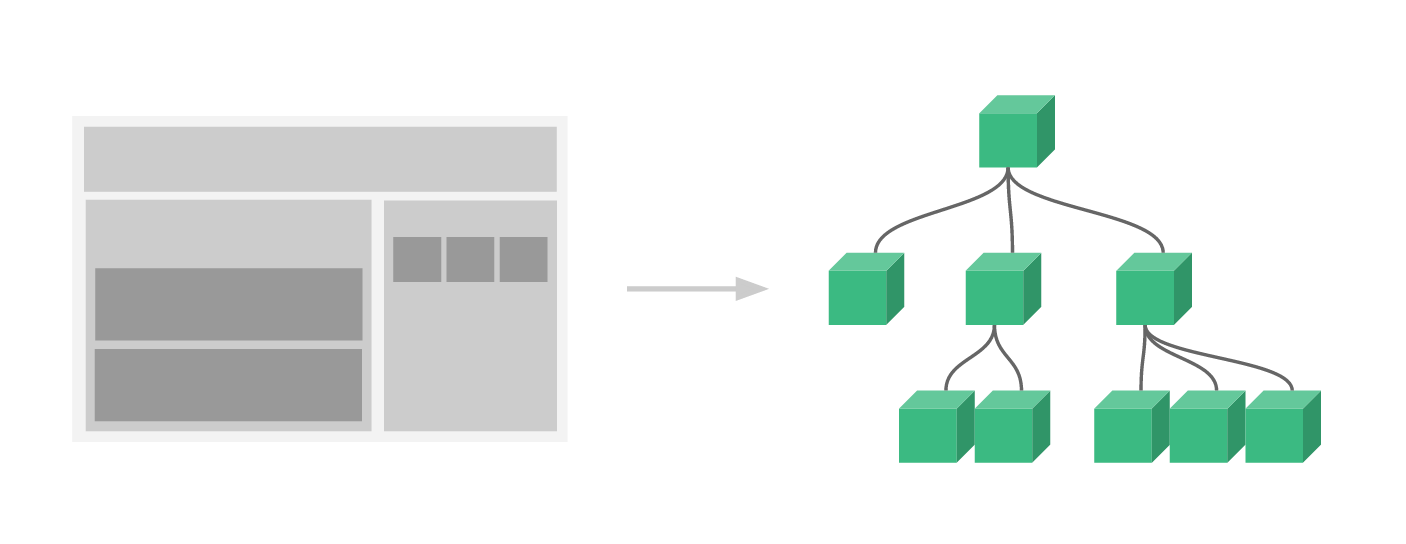
\includegraphics[width=0.9\textwidth]{Bilder/img/components.png}  
  \caption{ \textit{Organization of Componenten} \cite{VueComponents:Online}}%
\label{fig:OrganisationvonKomponenten}
\end{figure}

% Die grundlegende Struktur einer \texttt{Vue.js} Komponente ist im Listing \ref{lst:label} dargestellt. 

The template element contains the HTML template and the script element contains the JavaScript part of the component.
\begin{labeling}{Template element::}
	\item [Template element:] The design of the user interface is implemented in this element. Standard HTML and CSS technology are used for this. User-defined HTML elements, as well as HTML elements from external plug-ins, can be integrated very easily. The HTML-based template syntax of Vue.js allows binding the rendered DOM declaratively to the data of the underlying Vue instance. All Vue. js templates are valid HTML.
	
	The simplest form of data binding is text interpolation using the \textit{mustache} syntax (double curly braces):
	\begin{lstlisting}[language=html,label={lst:label}, caption=Templateelement]
        <template>
            <div>
                <h1>Data: {{ beispielData }}</h1>
                <BeispielComponent/>
            </div>
        </template>    
        \end{lstlisting}
		\item [Script element:] This element contains the implementation of the desired functionalities of the component with \texttt{VueJS} specific construct. Further components can be imported and registered here. These are then available in the template element, which allows the nesting of components to be realized.
	\begin{lstlisting}[language=JavaScript,label={lst:label}, caption=Skriptelement]
        
        <script>
          import BeispielComponent from 'components/BeispielComponent'
          export default {
            components: {
              BeispielComponent
            },
            props : [],
            data () {
              return {
                beispielData: 'Beispiel String'
              }
            },
            methods: {
                beispielFunction: function () { }
            },
            computed: {
            }
          }
        </script>
        
        \end{lstlisting}
\end{labeling}


The most important parts of a component are described in the table \ref{tab:table_data}.
\begin{table}[H]
	\centering
	\caption{Parameters responsible for data manipulation}
	\rowcolors{1}{}{gray!25}
	\label{tab:table_data}
	\begin{tabular}{{p{1.7cm}p{4cm}p{8cm}}}
		\toprule
		Parameters & Type & Description\\
        \midrule
        components & [key: string]: Object &This is a list of custom components to be used. The custom or external components are imported with \texttt{\textcolor{purple}{import}} command to import them from the ES6 specification.\\
		data & Object or Function & This is a JavaScript object or function that allows the storage of the necessary attributes for the component. Within the component, the original data object can be accessed with \texttt{\textcolor{purple}{this.data}} directive can be accessed.\\
		props & Array\(<string>\) or Object & This is a list/hash of attributes intended to hold data from the parent component. It has a simple array-based syntax and an alternative object-based syntax that allows advanced configurations such as type checking, custom validation and default values. \\
        methods & [key: string]: Function & This is a list of methods that allow the realisation of different functionalities of the component.  All methods can be called within the component as a standard JavaScript method.\\
        computed & [key: string]: Function & This is a list of methods that will be called automatically when the reactive dependencies change. The attributes within these parameters are cached and only recomputed on reactive dependency changes. \\
		\bottomrule
	\end{tabular}
\end{table}


\subsection{Instance lifecycle hooks}
\label{Vue:Instancelifecyclehooks} When created, each Vue instance goes through a series of initialization steps, e.g. it needs to set up data observation, compile the template, including the instance in the DOM and update the DOM when the data changes. In parallel, it also runs functions called lifecycle hooks that allow users to add their functions at certain stages of the instance lifecycle. This allows very precise control of the behavior of individual components.

For example, the \textit{created} hook can be used to execute code after an instance has been created. Other hooks are called at different stages of the instance lifecycle, such as. \textit{mounted}, \textit{updated} and \textit{destroyed}. The figure \ref{fig:OrganisationOfComponents} illustrates the details of the complete lifecycle hook.

\begin{figure}[H]
  \centering
  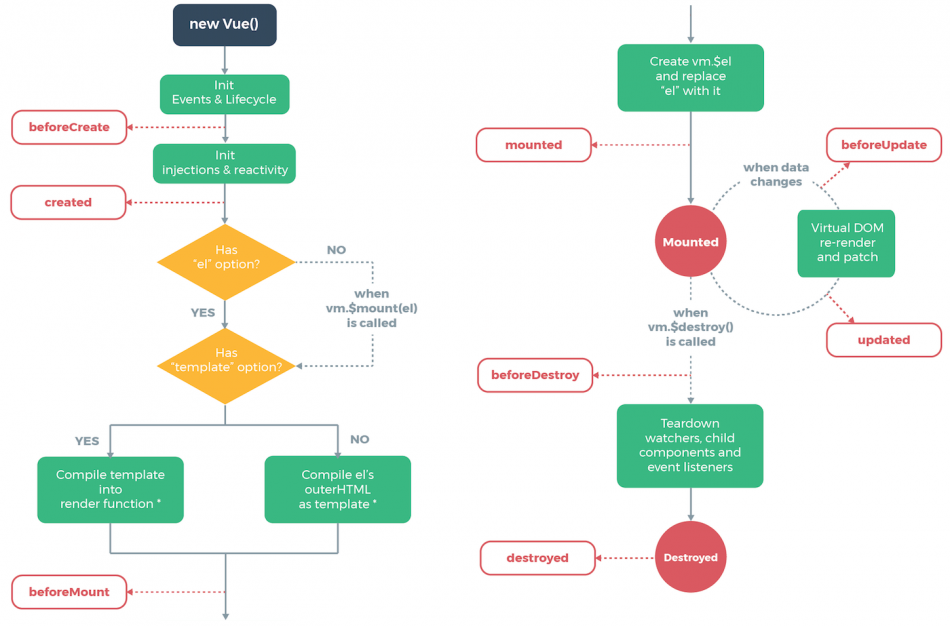
\includegraphics[width=1\textwidth]{Bilder/img/lifecycle_.png}  
  \caption{ \textit{Vue Instance-Lifecycle Hooks} \cite{InstancVue:Online}}%
\label{fig:OrganisationOfComponents}
\end{figure}



\subsection{Vuex }
\label{sec:Vuex}
Vuex is the official state management library for Vue. Its job is to exchange data between components in a Vue application.

Components in a Vue application can have their state. For example, an input field stores the data entered in it locally. Components can be input fields or a whole page. It becomes very costly to exchange state data between nested components.

Vuex provides central storage(Vuex store) for the state, and the state can be changed by calling functions defined in the Vuex store.
Each component that depends on a particular piece of state accesses it via a getter function on the Vuex store, ensuring synchronization of data. Vuex-Store is a kind of temporary database for a particular application session \cite{VueGuide:Online}.


\subsection{Vue Router }
\label{sec:Vue Router}

In a web application, a router is a part that synchronizes the currently displayed view with the contents of the browser address bar.

A router is needed when \gls{URL}s need to be synchronized with the views in an application. This is a very common need, and all major modern frameworks now allow routing to be managed.   Vue Router is part of the Vue core library and handles route management in a Vue application \cite{VueGuide:Online}.


\section{Nginx}
\label{Grundlagen:Nginx}
Nginx, pronounced like "engine-ex", is an open-source web server that is now also used as a reverse proxy, HTTP cache, and load balancer. It is one of the most used web servers along with the Apache HTTP server.\cite{nginxIntro}

This section describes the basics of NGINX (start, stop reload configuration), the structure of the configuration file and describes the process of setting up NGINX to serve out static content.

\subsection{Starting, Stopping, and Reloading Configuration}
Nginx has a single master process and several worker processes. The master process reads and evaluates the configuration and manages the worker processes. The worker processes operate the real processing of HTTP requests. Nginx uses an event-based model and operating system-dependent means to efficiently allocate requests among the worker processes. The number of worker processes is set in the configuration file.\cite{nginxIntro}


\subsection{Structure of Configuration File }
The configuration file is named by default nginx.conf and placed in the directory \textit{"/usr/local/nginx/conf", "/etc/nginx", or "/usr/local/etc/nginx"}. Nginx consists of modules that are controlled by directives defined in the configuration file. Directives are split into simple directives and block directives. A simple directive is made up of the name and parameters separated by spaces and ends with a semicolon (;). A block directive ends with a sequence of additional arguments surrounded by curly braces. A block directive that contains other directives inside curly braces, is called a context (examples: events, http, server, and location). Directives that are outside contexts in the configuration file are in the main context. The directives events and http are in the main context. The server directive is inside the http directive and location inside the server. For comments, a hashtag \lstinline{(#)} sign is used.\cite*{nginxIntro}

\subsection{Serving Static Content}

		
\chapter{Previous Work}

Masterarbeit von Christoph (Für DDS und Routing service)
	
	
	%
\section{Lösungsversprechen von Vue}
Vue wird zunächst als ein progressiver Framework bezeichnet.
Das bedeutet, dass es sich an die Bedürfnisse des Entwicklers anpasst.Während andere Frameworks eine vollständige Übernahme einer Technologie durch einen Entwickler oder ein Team erfordern und oft möchten, dass eine existierende Anwendung neu geschrieben wird, weil bestimmte Konventionen erforderlich sind. Vue landet zunächst mit einem einfachen Skript-Tag in einer Anwendung und kann mit den Anforderungen wachsen, von einer kleinen Web-Komponente bis hin zur Verwaltung der gesamten Ansichtsebene.
Es ist nicht notwendig, über Webpack, Babel, npm oder ähnliches Bescheid zu wissen, um mit Vue zu beginnen. HTML , CSS und Grundlagen von JavaScript reichen aus, um mit Vue anzufangen.

Der Sprung von einer reinen HTML- und CSS-basierten Website zu einer anspruchsvollen Webanwendung ist sehr einfach gehalten und kann im Laufe des Entwicklungsprozesses erlernt werden.
Dies ist ein starkes Verkaufsargument, insbesondere im aktuellen Ökosystem der JavaScript-Frontend-Frameworks und -Bibliotheken, das Neueinsteigern und auch erfahrenen Entwicklern das Gefühl gibt, im Ozean der Möglichkeiten und Wahlmöglichkeiten verloren zu gehen.
Das Ziel von Vue ist es, mit minimalem Vorkenntnisse vernünftige Web-Applikationen erstellen zu können.


{\let\clearpage\relax \chapter{Vue.js}}
% \chapter{Vue.js}
\label{sec:grundlagen}

Vue ist ein skalierbares JavaScript Framework zum Aufbau von Benutzeroberflächen. Im Gegensatz zu anderen Frameworks ist Vue von Grund auf so konzipiert, dass es schrittweise anpassbar ist. Die Kernbibliothek ist nur auf die Ansichtsebene (View) ausgerichtet und lässt sich leicht in andere Bibliotheken oder bestehende Projekte integrieren. In Kombination mit modernen Tools und zusätzlichen Bibliotheken, ist Vue  in der Lage, anspruchsvolle Single-Page-Applikationen zu betreiben \cite{Vue019:Intro:Online}.

\section[]{Haupt Merkmale }
\label{sec:Einführung}
% \subsection{VueJS}
% \label{sec:VueJS}


Vue ist zusammen mit React und Angular eines der beliebtesten Frameworks in der Webentwicklungslandschaft. Folgende Merkmale zeichnen das Vue-Framework aus:
\begin{labeling}{Components:::::}
	\item [Components:] Vue-Komponenten erweitern grundlegende \gls{HTML}-Elemente, um wiederverwendbaren Code zu kapseln. Das Vue-Komponenten-System ist eine Abstraktion, die die Erstellung großer Anwendungen aus kleinen, in sich geschlossenen und oft wiederverwendbaren Komponenten ermöglicht.
	\item [Templates:] Vue.js verwendet eine HTML/\gls{CSS}-basierte Template-Syntax. Vue kompiliert  die Vorlagen (Templates) in virtuelle \gls{DOM}-Renderfunktionen. In Kombination mit dem Reaktivitätssystem ist Vue in der Lage, intelligent die minimale Anzahl von Komponenten, die aktualisiert werden müssen, zu ermitteln. Dies minimiert die Anzahl von DOM-Manipulationen bei der Zustandsänderung der Applikation.
	\item [Reaktivität:] Vue verfügt über ein Reaktivitätssystem, welches reine JavaScript-Objekte verwendet und das Rendering optimiert. Jede Komponente behält während des Renderns den Überblick über ihre reaktiven Abhängigkeiten. Das ermöglicht dem System intelligent und optimal die Komponenten neu zu rendern.
  \item [Integrierbarkeit:] Es ist sehr einfach, Vue in bestehende Projekte zu integrieren oder Bibliotheken von Drittanbietern zu Vue hinzuzufügen. Alle JavaScript-Bibliotheken, die ES6+ verwenden, können innerhalb von Vue verwendet werden. Zum Beispiel Bootstrap, Material Design, ThreeJS, Web Sensors API usw.  Vue bietet auch die Möglichkeit, TypeScript anstelle von JavaScript zu verwenden.
	
\end{labeling}
\cite{VueGuide:Online}

\section{Vue im Vergleich zu Angular und React}
\label{sec:Vue im Vergleich zu Angular und React}
 Vue wurde von Evan You entwickelt, als er bei Google an AngularJS (Angular 1.0)-Anwendungen arbeitete.Vue übernahm einen Teil der Angular-Templating-Syntax aus, entfernte jedoch den komplexen Stack, den Angular erforderte. Dadurch wurde es sehr leistungsfähig. Das neue Angular (Angular 2.0) löste auch viele der AngularJS-Probleme, jedoch auf sehr unterschiedliche Weise, und erfordert TypeScript, das nicht alle Entwickler gerne verwenden (oder lernen wollen).

Vue hat viele gute Ideen von React übernommen, vor allem das virtuelle DOM.  Aber Vue implementiert es mit einer Art automatischer Abhängigkeitsverwaltung, die nachverfolgt, welche Komponenten von einer Änderung des Zustands betroffen sind, so dass nur diese Komponenten neu gerendert werden, wenn sich die Zustands-Eigenschaft ändert. In React hingegen wird bei einer Änderung eines Teils des Zustandes, der Auswirkungen auf eine Komponente hat, diese Komponente neu gerendert, und damit werden auch alle zugehörigen Kinder-Komponente neu gerendert. Dies ist ein Vorteil für Vue in Bezug auf die Benutzerfreundlichkeit und die Leistungssteigerung \cite{VueComparision:Online}.

\begin{table}[H]
	\centering
	\caption{Vue vs React vs Angular}
	\label{tab:table_VueJS}
	\begin{tabular}{{p{3cm}|p{3cm}|p{3cm}|p{3cm}}}
    \toprule
    Kriterium & 
\includegraphics[width=0.05\textwidth]{Bilder/img/vue.png} & 
\includegraphics[width=0.05\textwidth]{Bilder/img/react.png} & 
\includegraphics[width=0.05\textwidth]{Bilder/img/angular.png}\\
     & Vue & React & Angular\\
    \midrule
    Fokus & Nutzbarkeit & Flexibilität & TypeScript \\
    Komplexität & Niedrig & Mittel & Hoch \\
    Größe & 80 KB & 100 KB  & 500+ KB\\
    Veröffentlichung & 2014 & 2013  & 2010 \\
    Entwickelt von & Evan You & Facebook & Google \\
    Sprache & JavaScript & JavaScript & TypeScript\\
    Model & virtuelle DOM & virtuelle DOM & \gls{MVC}\\
    Unterstütz von & Open Source & Facebook  & Google \\
    Aktuellste Version & 2.6.11 & 16.13.1 & 9.1.11\\
		\bottomrule
	\end{tabular}
\end{table}
\cite{ComparisonVue:Online}


\section{Struktur eines Vue.js Projekts}
\label{sec:Struktur eines Vue.js Projekts}
Vue hat eine sehr intuitive Projektstruktur. Zusätzlich zum Kern des Frameworks enthält es eine Menge Utilities, die die Frontend-Entwicklung mit Vue sehr angenehm machen.
Wie meisten JavaScript Projekte wird für Vue-Entwicklung NodeJS verwendet. Vue stellt die Kernbibliothek und die Zusatz Utilities über \texttt{\textbf{\gls{npm}} (node package manager)} zur Verfügung.

\paragraph{NodeJS} ist eine JavaScript-Laufzeitumgebung, die auf der V8-JavaScript-Engine von Chrome basiert. Sie ermöglicht die Ausführung von JavaScript-Code außerhalb eines Webbrowsers. NodeJS ermöglicht es Entwicklern, JavaScript zum Schreiben von Kommandozeilen-Tools und für die serverseitige Ausführung von Skripten zu verwenden, um dynamische Webseiteninhalte zu erzeugen, bevor die Seite an den Webbrowser des Benutzers gesendet wird. NodeJS unterstützt die Vereinheitlichung der Web-Anwendungsentwicklung um eine einzige Programmiersprache herum, anstatt verschiedene Sprachen für server- und clientseitige Skripte zu verwenden \cite{NodeJS:Online}.

\paragraph{npm (node package manager)} ist die größte Software-Registry der Welt. Open-Source-Entwickler aus allen Kontinenten nutzen npm, um Pakete gemeinsam zu nutzen und auf sie zuzugreifen, und viele Organisationen nutzen npm auch zur Verwaltung der privaten Entwicklung \cite{NPM:Online}.

\paragraph*{Vue-CLI:} Vue bietet eine offizielle CLI(Command Line Interface) für das schnelle Einrichten anspruchsvoller einseitiger Anwendungen. Es bietet einen umfassenden Build-Setup für einen modernen Frontend-Workflow. Es dauert nur wenige Minuten, um mit Hot-Reload, Lint-on-Save und Produktions-Builds in Betrieb zu gehen.

\paragraph{Installiation}
Die Installation der erforderlichen Pakete wird mit NodeJS und npm durchgeführt. Folgende Befehle müssen ausgeführt werden um ein Basis Vue Anwendung zu erstellen:
\begin{itemize}
  \item Die Vue-CLI global installieren:
  \begin{lstlisting}[language=bash]
    npm install -g @vue/cli
  \end{lstlisting}
  \item Die Vue-\gls{CLI} wird verwendet um einen neuen Vue-Projekt zu erstellen.
  \begin{lstlisting}[language=bash]
    vue create beispiel_vue_app
  \end{lstlisting}
  Dadurch wird eine CLI geöffnet, in der die gewünschte Konfiguration für ein Vue-Projekt eingestellt werden kann.
  \item Um den Entwicklungsserver zu starten, wird der folgende Befehl ausgeführt:
  \begin{lstlisting}[language=bash]
    npm run serve
  \end{lstlisting}
  \item Um einen Production-Build für die App zu erzeugen, wird folgender Befehl ausgeführt:
  \begin{lstlisting}[language=bash]
    npm run build
  \end{lstlisting} 
\end{itemize} 

Ein typisches Vue-Projekt mit Vue-Router und Vuex hat die folgende Struktur:

\begin{table}[H]
	\centering
	\caption{Struktur des Projektordners}
	\label{tab:table_VueJS}
	\begin{tabular}{{p{4cm}p{9cm}}}
		\toprule
		Dateien/Ordner  & Beschreibung\\
		\midrule
    public/index.html & Dies ist die Haupt-App-Datei, die vom Browser geladen wird. 
    Die Datei enthält im Body nur ein einfaches HTML-Tag: \texttt{ \textcolor{red}{<div id=\enquote{app}> </div>}}. 
    Dies ist das Element, mit dem die Vue-Anwendung an das DOM angehängt wird. \\
    \hline
    src/main.js & Dies ist die JavaScript-Datei, die für die Konfiguration der Vue.js Anwendung verantwortlich ist. Es wird auch verwendet, um alle Pakete von Drittanbietern zu registrieren. \\
    \hline
    src/App.vue & Dies ist die Root-Komponente, die den HTML-Inhalt enthält, der dem Benutzer angezeigt wird. \\
    \hline
    /package.json & In dieser Datei speichert npm die Namen und Versionen des Pakets, das es installiert hat. \\
    \hline
    src/components/ & Dieser Ordner enthält die zusätzlichen Komponenten. \\
    \hline
		src/assets/ & Dieser Ordner wird verwendet, um statische Inhalte, wie Bilder zu speichern. \\
    \hline
		src/router/ & Der Ordner enthält die Implementierung von Vue-Router. \\
		\hline
		src/store/ & Der Ordner enthält die Implementierung von Vuex-Store. \\
    \bottomrule
	\end{tabular}
\end{table}

% \begin{lstlisting}[language=JavaScript, caption=package.json]
% {
%   "name": "vue_pwa",
%   "version": "0.1.0",
%   "scripts": {
%     "serve": "vue-cli-service serve",
%     "build": "vue-cli-service build",
%   },
%   "dependencies": {
%     "vue": "^2.6.11",
%     "vue-router": "^3.1.6",
%     "vuetify": "^2.2.11",
%     "vuex": "^3.1.3"
%   },
%   "devDependencies": {
%     "@vue/cli-plugin-router": "~4.3.0",
%     "@vue/cli-plugin-vuex": "~4.3.0",
%     "@vue/cli-service": "~4.3.0",
%   },
% }

% \end{lstlisting}
\section{Das Vue Instanz} Jede Vue-Anwendung beginnt mit der Erstellung einer neuen Vue-Instanz (Root Instance) mit der Vue-Funktion. Wenn eine Vue-Instanz erstellt wird, fügt sie dem Reaktivitätssystem von Vue alle in ihrem Datenobjekt(beschrieben in Tabelle \ref{tab:table_data}) gefundenen Eigenschaften hinzu.  Alle zu verwendende \texttt{Vue.js} internen Module und externen Plugins werden in der Datei \texttt{(main.js)} mit ES6(ECMAScript 2015) Import Syntax ('import') importiert. Die Abhängigkeiten sind als globale Parameter definiert und sind von allen Komponenten zugänglich.  
% Ein typischer VueJS Projekt hat eine Struktur wie im Abbildung \ref{fig:vue_projekt_struktur}. 
In der main.js Datei wird die Haupt-Vue-Komponente (\texttt{App.vue}) registriert. 
%Die Funktion der einzelnen Dateien in dem Projektordner sind in der Tabelle \ref{tab:table_VueJS} beschrieben.
\begin{lstlisting}[language=JavaScript, caption=main.js]
    import Vue from 'vue'
    import App from './App'
    import router from './router'

    // Root Instance
    new Vue({
        el: '#app',
        router,
        template: '<App/>',
        components: { App }
    })

\end{lstlisting}

\section{Vue Komponente}Das wichtigste Kriterium für die Auswahl dieses Frameworks \texttt{(Vue.js)} ist die Modularität der einzelnen Komponenten (beschrieben im Abschnitt \ref{sec:Einführung}). Die Komponenten sind eine der stärksten Eigenschaften von \texttt{Vue.js}. Sie ermöglichen, grundlegende HTML-Elemente zu erweitern, um wiederverwendbaren Code zu kapseln. Auf einer hohen Ebene sind Komponenten benutzerdefinierte Elemente, an die der \texttt{Vue.js} Compiler ein bestimmtes Verhalten anhängt \cite{Vue019:Intro:Online}. Jede Komponente wird in einer Datei mit \texttt{.vue} Erweiterung definiert. Die Definition enthält ein HTML basiertes Template, die die Gestaltung der Komponente festlegt und den JavaScript Code, das alle andere Funktionalitäten bzw. Verhalten der Komponente spezifiziert. Jede Komponente ist ebenfalls eine Vue-Instanz.

Üblicherweise wird eine Vue.js App in einem Baum aus verschachtelten Komponenten organisiert. Beispielsweise besteht sie aus Komponenten für einen Header, eine Seitenleiste und einen Inhaltsbereich, die jeweils andere Komponenten für Navigationslinks, Blog-Posts usw. enthalten. Die Komponenten Architektur vereinfacht solche Verschachteltelung.
\begin{figure}[H]
  \centering
  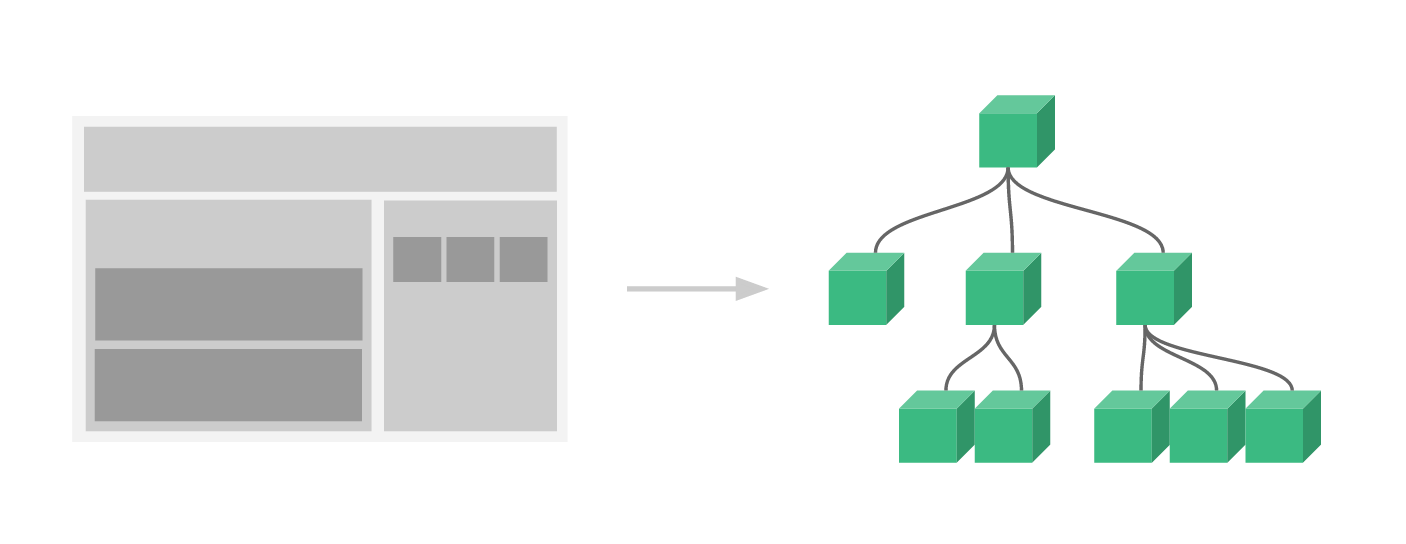
\includegraphics[width=0.6\textwidth]{Bilder/img/components.png}  
  \caption{ \textit{Organisation von Komponenten} \cite{VueComponents:Online}}%
\label{fig:Organisation von Komponenten}
\end{figure}

% Die grundlegende Struktur einer \texttt{Vue.js} Komponente ist im Listing \ref{lst:label} dargestellt. 

Das Template-Element beinhaltet das HTML-Template und das Script-Element beinhaltet den JavaScript-Teil der Komponente.
\begin{labeling}{Template-Element::}
	\item [Template-Element:] Die Gestaltung bzw. das Design der Benutzeroberfläche wird in deisem Element implementiert. Dafür wird Standard HTML und CSS Technik verwendet. Es können sowohl benutzerdefinierte HTML-Element als auch HTML-Elemente aus externen Plugins sehr einfach integriert werden. Die HTML-basierte Template-Syntax von Vue.js ermöglicht es, das gerenderte DOM deklarativ an die Daten der zugrunde liegenden Vue-Instanz zu binden. Alle Vue. js-Templates sind gültiges HTML.
	
	Die einfachste Form der Datenbindung ist die Textinterpolation unter Verwendung der \enquote{Mustache}-Syntax (doppelte geschweifte Klammern):
	\begin{lstlisting}[language=html,label={lst:label}, caption=Templateelement]
        <template>
            <div>
                <h1>Data: {{ beispielData }}</h1>
                <BeispielComponent/>
            </div>
        </template>    
        \end{lstlisting}
	\item [Script-Element:] Dieses Element beinhaltet die Implementierung der gewünschten Funktionalitäten der Komponente mit \texttt{VueJS} spezifischem Konstrukt. Weitere Komponenten können hier importiert und registriert werden. Diese stehen dann im Template-Element zur Verfügung, welches die Verschachtelung von Komponenten realisieren lässt.
	\begin{lstlisting}[language=JavaScript,label={lst:label}, caption=Skriptelement]
        
        <script>
          import BeispielComponent from 'components/BeispielComponent'
          export default {
            components: {
              BeispielComponent
            },
            props : [],
            data () {
              return {
                beispielData: 'Beispiel String'
              }
            },
            methods: {
                beispielFunction: function () { }
            },
            computed: {
            }
          }
        </script>
        
        \end{lstlisting}
\end{labeling}


Die wichtigsten Teile einer Komponente sind in der Tabelle \ref{tab:table_data} beschrieben.
\begin{table}[H]
	\centering
	\caption{Parameter zuständig für Datenmanipulation}
	\label{tab:table_data}
	\begin{tabular}{{p{1.7cm}p{4cm}p{8cm}}}
		\toprule
		Parameter & Typ & Beschreibung\\
        \midrule
        components &[key: string]: Object &Dies ist eine Liste von zu verwendenden benutzerdefinierten Komponenten. Die benutzerdefinierten bzw. externen Komponenten werden mit \texttt{\textcolor{purple}{import}} Befehl aus ES6 Spezifikation importiert.\\
		data & Object | Function & Dies ist ein JavaScript Objekt oder eine Funktion, die die Speicherung der notwendigen Attribute für die Komponente erlaubt. Innerhalb der Komponente kann auf das ursprüngliche Datenobjekt mit \texttt{\textcolor{purple}{this.data}} Direktive zugegriffen werden.\\
		props&Array<string> | Object & Dies ist eine Liste/Hash von Attributen, die zur Aufnahme von Daten aus der übergeordneten Komponente vorgesehen sind. Es hat eine einfache Array-basierte Syntax und eine alternative Objekt-basierte Syntax, die erweiterte Konfigurationen wie Typprüfungen, benutzerdefinierte Validierung und Standardwerte ermöglicht. \\
        methods&[key: string]: Function  & Dies ist eine Liste von Methoden, die die Realisierung verschiedener Funktionalitäten der Komponente erlauben.  Alle Methoden können innerhalb der Komponente als eine standard JavaScript Methode aufgerufen werden.\\
        computed&[key: string]: Function & Dies ist eine Liste von Methoden, die automatisch bei Änderung der reaktiven Abhängigkeiten aufgerufen wird. Die Attribute innerhalb dieser Parameter werden zwischengespeichert und nur bei reaktiven Abhängigkeitsänderungen neu berechnet. \\
		\bottomrule
	\end{tabular}
\end{table}


\section{Instanz-Lebenszyklus Hooks} Bei der Erstellung durchläuft jede Vue-Instanz eine Reihe von Initialisierungsschritten, z. B. muss sie die Datenbeobachtung einrichten, die Template kompilieren, die Instanz in das DOM einbinden und das DOM aktualisieren, wenn sich die Daten ändern. Parallel dazu werden auch Funktionen ausgeführt, die als Lifecycle-Hooks bezeichnet werden und den Benutzern die Möglichkeit geben, in bestimmten Phasen des Instanz-Lebenszyklus ihren eigenen Funktionen hinzuzufügen. Dies ermöglicht eine sehr präzise Steuerung des Verhaltens einzelner Komponenten.

Der \enquote{created} Hook kann beispielsweise zur Ausführung von Code nach der Erzeugung einer Instanz verwendet werden. Es gibt auch andere Hooks, die in verschiedenen Phasen des Lebenszyklus der Instanz aufgerufen werden, wie z.B. \enquote{mounted}, \enquote{updated} und \enquote{destroyed}. Die Abbildung \ref{fig:Organisation von Komponenten} illustriert die Details des kompletten Lifecycle-Hooks.

\begin{figure}[H]
  \centering
  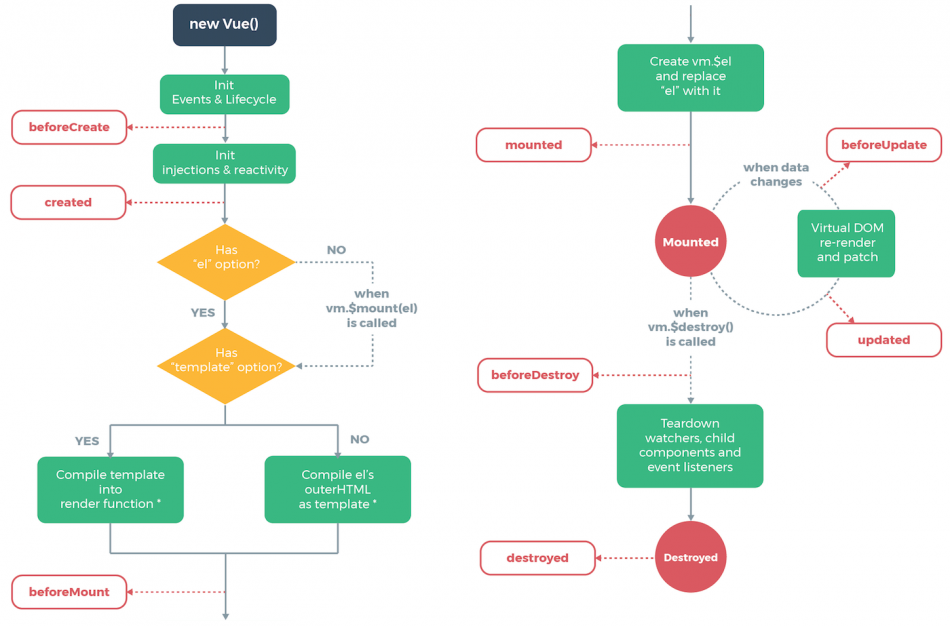
\includegraphics[width=1\textwidth]{Bilder/img/lifecycle_.png}  
  \caption{ \textit{Vue Instanz-Lifecycle Hooks} \cite{InstancVue:Online}}%
\label{fig:Organisation von Komponenten}
\end{figure}





% \begin{figure}[H]
% 	\centering
% 	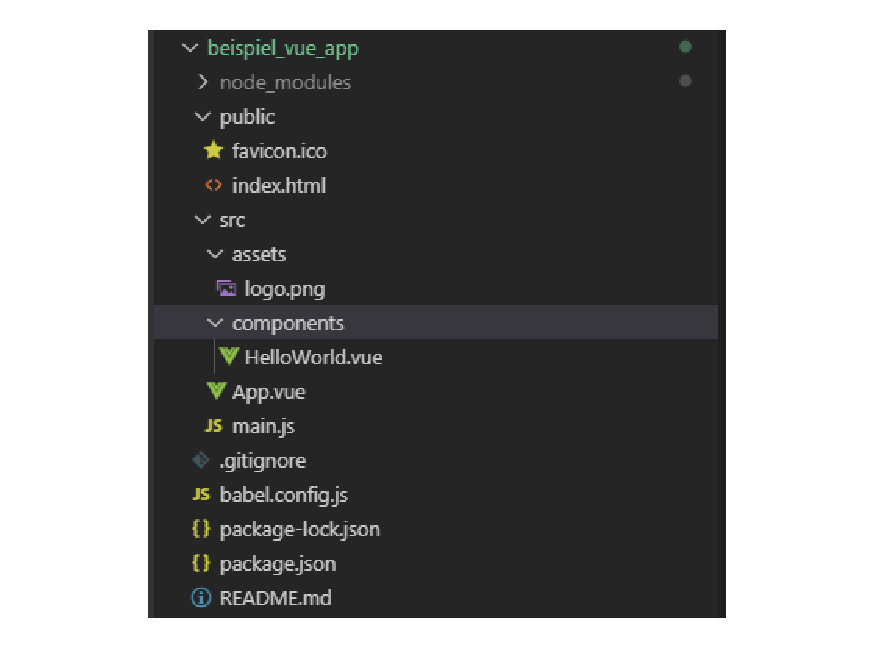
\includegraphics[width=1\textwidth]{img/vue_projekt_struktur.pdf}  
% 	\caption{ \textit{Vue.Js Projekt Struktur}}%
% \label{fig:vue_projekt_struktur}
% \end{figure}


\section{Vuex }
\label{sec:Vuex}
Vuex ist die offizielle Zustandsverwaltungsbibliothek für Vue. Ihre Aufgabe besteht darin, Daten zwischen den Komponenten einer Vue Anwendung auszutauschen.

Komponenten in einer Vue-Anwendung können ihren eigenen Zustand haben. Beispielsweise speichert ein Eingabefeld die darin eingegebenen Daten lokal. Komponenten können eine Eingabefeld sein oder eine ganze Seite. Es wird sehr aufwendig die Zustandsdaten zwischen verschachtelten Komponenten auszutauschen.

Vuex bietet einen zentralen Repository-Speicher(Vuex-Store) für den Zustand, und der Zustand kann durch den Aufruf von im Vuex-Store definierten Funktionen geändert werden.
Jede Komponente, die von einem bestimmten Teil des Zustands abhängt, greift auf diesen über einen getter Funktion auf dem Vuex-Store zu, wodurch Synchronisierung der Daten sichergestellt wird. Vuex-Store ist eine Art temporäre Datenbank für eine bestimmte Anwendungssitzung \cite{VueGuide:Online}.


\section{Vue Router }
\label{sec:Vue Router}

In einer Webanwendung ist ein Router der Teil, der die aktuell angezeigte Ansicht mit dem Inhalt der Browser-Adressleiste synchronisiert.

Ein Router wird benötigt, wenn \gls{URL}s mit den Ansichten in einer Anwendung synchronisiert werden müssen. Dies ist eine sehr häufige Notwendigkeit, und alle wichtigen modernen Frameworks erlauben inzwischen die Verwaltung des Routings.   Vue Router ist Teil der Vue Kern Bibliothek und übernimmt die Routenverwaltung in einer Vue-Anwendung \cite{VueGuide:Online}.

\newpage
{\let\clearpage\relax \chapter{Evaluation}}

Als Prototyp zum Testen der oben genannten Technologie wurde eine Einkaufsliste App entwickelt. Das Grundlayout wurde unter Verwendung von Standard-HTML und CSS entwickelt, und der Inhalt der Einkaufsliste wurde mit der Textinterpolations-Funktion von Vue implementiert. Jedes Element in der Einkaufsliste ist eine Vue-Komponente. Die entwickelte App verwendet die von Vue angebotene verschachtelte Komponentenarrhitektur. Vuex wird verwendet, um die Daten in der Einkaufsliste zu verwalten.
Der Quellcode der Prototyp-Anwendung, die mit dieser Technologie entwickelt wurde, ist in diesem Git-Repository zu finden: \url{https://git.efi.th-nuernberg.de/gitea/yadavaa81855/vue_pwa.git}

Es war insgesamt eine sehr angenehme Erfahrung, die App zu entwickeln. Wirklich gute Dokumentation und einfache Anwendbarkeit des Frameworks machen die Lernkurve ziemlich flach. Die Integration von Drittbibliotheken ist nicht kompliziert. Es war nicht notwendig, alles über das Framework zu lernen, um eine einfache App zu erstellen, und neue Funktionen können der App mit Hilfe dieses Frameworks leicht hinzugefügt werden.

\begin{table}[H]
	\centering
	\caption{Bewertung von VueJS anhand entwickelte Prototyp}
	\label{tab:table_VueJS}
	\begin{tabular}{{p{3cm}p{10cm}}}
		\toprule
		Kriterien  & Bewertung\\
		\midrule
		Lernkurve & In der Entwicklung überzeugt Vue.js durch die gute Erlernbarkeit der verschiedenen Konzepte, die aufeinander aufbauen.  \\
		\hline
    Modularität & Das Kern-Framework ist also sehr schlank und überschaubar und hat nur wenige Grundbausteine. Zusätzliche Funktionalitäten können mit Hilfe von Zusatzmodulen hinzugefügt werden \\
    \hline
    Skalierbarkeit & Es kann verwendet werden, um kleine Websites bis hin zu anspruchsvollen Webanwendungen zu erstellen. \\
    \hline
		Ökosystem & Vue.js verfügt über ein umfassendes Ökosystem mit Unterstützung für Bibliotheken und Plugins von Drittanbietern. \\
    \bottomrule
	\end{tabular}
\end{table}

 \chapter{Fazit}
Vue.js ist vielleicht nicht das am weitesten entwickelte Framework, aber es erfüllt manche Anforderungen vollkommen richtig. Erstens können sehr schnell und ohne großen Aufwand schöne Widgets und Anwendungen geschrieben werden. Die Lernkurve ist niedrig, das Belohnungsgefühl ist enorm hoch. Anfänger werden ihren Spaß mit Vue.js haben, vor allem weil alles so überschaubar ist.
Vue.js skaliert auch mit den Bedürfnissen des Teams und dem Wissensstand des Entwicklers und wird von der Entwickler-Community gut angenommen. 

Die Komponentenarchitektur von Vue.js hilft, die Anwendung so zu strukturieren, dass es einfach ist, durch die Teile der Anwendung zu navigieren, die von anderen Entwicklern entwickelt wurden. Die robusten \gls{API}s ermöglichten es, sich auf die Implementierung der Geschäftslogik zu konzentrieren, anstatt sich mit dem Framework zu befassen.

Vue.js verfügt über eine ausgezeichnete Online-Dokumentation mit vielen Beispielen.  Zusätzlich gibt es einen Vue.js Style Guide, der Best Practices zeigt, ein Vue.js-Kochbuch, das häufig verwendete Muster beschreibt, und eine Übersicht über zusätzliche Bibliotheken und Vue.js-Erweiterungen.
	
	\chapter{Design and Implementation}
\label{Implementation}

This chapter describes the Design process and the details of the realized implementation of a Docker based application developed for managing ROS2 nodes in a local Network over a web interface. Figure \ref*{fig:Background:LifecycleManagement} provides an overview of the Structure of the developed application. The application is supposed to have control over all the compatible ROS2 Applications running within a defined network. It utilizes the ROS2 DDS System (for communication within same LAN) and ROS2 Routing Service (for communication between different Networks). It consists of a customized ROS2 based Docker Containers within which individual ROS2 applications run and another customized Docker Container running a NodeJS based Web-Application (Lifecycle Management Dashboard).   

\begin{figure}[H]
	\centering
	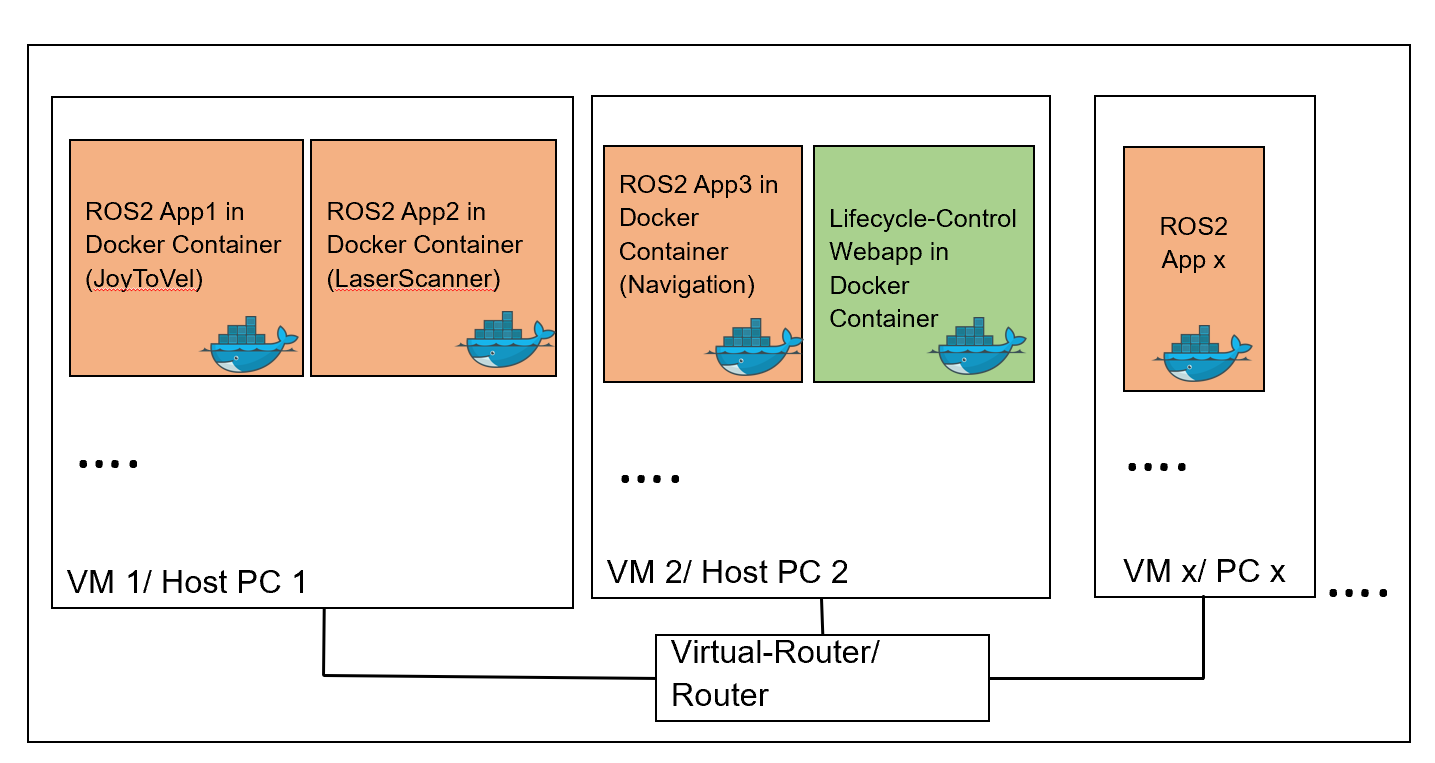
\includegraphics[width=0.95\textwidth]{"Bilder/Application-Structure.png"}
	\caption{Structure of Lifecycle Management Application}
	\label{fig:Background:LifecycleManagement}					
\end{figure}
The application consists of following major parts:

\begin{itemize}
	\item The Docker environment
	\item ROS2 Lifecycle Application
	\item Web-Interface
	\item Integration
\end{itemize}

They will be explained in detail in the following section.
\newpage
\section{The Docker environment}
\label{Implementierung:DockerEnvironment}
In order to develop an Industrial Edge Application, its necessary to pack an application into a Docker Image. Then it can be converted to an Industrial Edge Application using the Industrial Edge Application Publisher.\\

This section describes the Docker image developed for the purposes of this thesis. A Dockerfile is used to define a Docker image. It consists of all the necessary software libraries and third party applications and precise order in which they have to installed. The following section will describe the details of the Dockerfile(structure of the Docker image) step by step.
\subsection{The Dockerfile}
This section consists of a detailed description of the major blocks of steps performed to create the desired docker image of this application.
\paragraph{Setting up the Base-Image} This is the first line in any Dockerfile. In this line the Ubuntu ROS Image to use is specified.
\begin{lstlisting}[language=docker,
	% caption={Dockerfile}, 
	label={code:DockerTestumgebung}]
	FROM ros:foxy-ros-core-focal
\end{lstlisting}


\paragraph{Installing Bootstrap Tools} This step installs the Bootstrap Tools(apt-utils, build-essentials, nano, git, curl, tmux) and necessary python3 extensions (python3-colcon-common-extensions, python3-colcon-mixin, python3-rosdep, python3-vcstool)

\begin{lstlisting}[language=docker,
	% caption={Dockerfile}, 
	label={code:DockerTestumgebung}]
	# install bootstrap tools
	RUN apt-get update && apt-get install -y --no-install-recommends \
		apt-utils \
		build-essential \
		nano \
		git \
		curl \
		tmux \
		inetutils-ping \
		python3-colcon-common-extensions \
		python3-colcon-mixin \
		python3-rosdep \
		python3-vcstool \
		&& rm -rf /var/lib/apt/lists/*

\end{lstlisting}

\paragraph{Setting up ROS Build environment} The rosdep is initialized and updated before installing any ROS2 Package. Then colcon mixin and metadata are setup and any related libraries are updated. Colcon is the default and recommended build system for ROS2. Now ROS2 applications can be built using colcon in the next step.\newpage
\begin{lstlisting}[language=docker,
	% caption={Dockerfile}, 
	label={code:DockerTestumgebung}]
	# bootstrap rosdep
	RUN rosdep init && \
	rosdep update --rosdistro $ROS_DISTRO
	# setup colcon mixin and metadata
	RUN colcon mixin add default \
		https://raw.githubusercontent.com/colcon/
		colcon-mixin-repository/master/index.yaml && \
		colcon mixin update && \
		colcon metadata add default \
		https://raw.githubusercontent.com/colcon/
		colcon-metadata-repository/master/index.yaml && \
		colcon metadata update
\end{lstlisting}

\paragraph*{Installing necessary ROS packages} Following ROS2 Packages are installed in this step: ros-foxy-ros-base=0.9.2-1*, ros-foxy-joy, ros-foxy-diagnostic-updater,ros-foxy-lifecycle. Depending on the type of ROS2 application it might be necessary to install further Packages, which should be done in this to avoid further complications. Finally, the system is updated to fix any broken installs and install any missing libraries.
\begin{lstlisting}[language=docker,
	% caption={Dockerfile}, 
	label={code:DockerTestumgebung}]
	# install ROS2 packages
	RUN apt-get update && apt-get install -y --no-install-recommends \
		ros-foxy-ros-base=0.9.2-1* \
		ros-foxy-joy \
		ros-foxy-diagnostic-updater \
		# install for lifecycle 
		ros-foxy-lifecycle \
		nginx \
		python \
	# update system
		&& apt-get upgrade -y \
		&& rm -rf /var/lib/apt/lists/* 
\end{lstlisting}


\paragraph*{Sourcing ROS2} Sourcing is a common term among UNIX users. In order to make the desired changes applicable to the current shell , it is necessary to "source" the file. Furthermore adding sources to .bashrc files preconfigures any new shell opened. In this step ROS2 setup files are sourced so that other ROS2 commands can be run from the command line. 
\begin{lstlisting}[language=docker,
	% caption={Dockerfile}, 
	label={code:DockerTestumgebung}]
	#add sources to bashrc
	RUN echo "source /opt/ros/foxy/setup.bash" >> ~/.bashrc \
		&& echo "source /root/colcon_ws/install/setup.bash" >> ~/.bashrc
\end{lstlisting}

\paragraph*{Create and build ROS Workspace} In this step, first of all the build workspace is setup, then the necessary source files are copied from external working directory to the Docker internal workspace and finally built using colcon.
\begin{lstlisting}[language=docker,
	% caption={Dockerfile}, 
	label={code:DockerTestumgebung}]
	# create and build workspace
	ENV ROS2_WS /root/colcon_ws
		
	COPY ./evo_siemensrob_ctrl ${ROS2_WS}/src/evo_siemensrob_ctrl/.
	COPY ./joy_converter ${ROS2_WS}/src/joy_converter/.
	COPY ./joytovel ${ROS2_WS}/src/joytovel/.
	COPY ./twist_mux ${ROS2_WS}/src/twist_mux/.

	RUN cd ${ROS2_WS} \
		&& . /opt/ros/foxy/setup.sh \
		&& colcon build
		
	# install RIB support
	COPY ./RIBInstall .

	RUN ./RIBInstall \
		&& rm -rf RIBInstall
\end{lstlisting}

\paragraph{Setup NodeJS environment for Vue} This step installs a version of NodeJS in this Docker environment. NodeJS will be necessary to build the Vue-application and run ros2-web-bridge in forthcoming steps. 
\begin{lstlisting}[language=docker,
	% caption={Dockerfile}, 
	label={code:DockerTestumgebung}]
	# For Lifecycle-Dashboard Vue App
	ENV NODE_VERSION=12.6.0
	# Already installed RUN apt install -y curl
	RUN curl -o- https://raw.githubusercontent.com/
	creationix/nvm/v0.34.0/install.sh | bash
	ENV NVM_DIR=/root/.nvm
	RUN . "$NVM_DIR/nvm.sh" && nvm install ${NODE_VERSION}
	RUN . "$NVM_DIR/nvm.sh" && nvm use v${NODE_VERSION}
	RUN . "$NVM_DIR/nvm.sh" && nvm alias default v${NODE_VERSION}
	ENV PATH="/root/.nvm/versions/node/v${NODE_VERSION}/bin/
	:${PATH}"
	RUN node --version
	RUN npm --version
\end{lstlisting}



\paragraph{Copy package.json files to install NodeJS project dependencies} A package.json file is a standard package specification file for NodeJS applications. It contains all the necessary configurations and list of packages to successfully build a NodeJS application. In this step 
a working directory for the Vue Application is created, the the package.json is copied to the Docker internal work directory and finally the project dependencies are downloaded and installed.
\begin{lstlisting}[language=docker,
	% caption={Dockerfile}, 
	label={code:DockerTestumgebung}]
	# build stage
	WORKDIR /app
	COPY ./lifecycle-dashboard/package*.json ./
	RUN npm install
\end{lstlisting}

\paragraph*{Build the web application for production} The project source files for the "Lifecycle management application" are copied from external workspace to the Docker work directory and built for production.
\begin{lstlisting}[language=docker,
	% caption={Dockerfile}, 
	label={code:DockerTestumgebung}]
	# build stage
	COPY ./lifecycle-dashboard/ .
	RUN npm run build
\end{lstlisting}

\paragraph{Setting up a Nginx web server} In this step the nginx configuration file (described in section \ref{Impl:NginxConfig}) is copied from external workspace to the docker environment. The built application consisting of only .html, .css and .js files are copied to a location where nginx can easily find them and use them to start the web-application. Furthermore PORT 80 is exposed and the web-application can thus be accessed on localhost:8080 within the same network where this Docker container is running.
\begin{lstlisting}[language=docker,
	% caption={Dockerfile}, 
	label={code:DockerTestumgebung}]
	# For nginx
	COPY ./nginx.conf /etc/nginx/nginx.conf
	RUN cp -a /app/dist/. /var/www/html
	EXPOSE 80
\end{lstlisting}

\paragraph*{Installing ros2-web-bridge} In this step ros2-web-bridge is installed and other services that need to launch at startup are setup. The web-server(nginx) is setup to start at launch.
\begin{lstlisting}[language=docker,
	% caption={Dockerfile}, 
	label={code:DockerTestumgebung}]
	
	# install ros2-web-bridge

	# set workdirectory as /root
	WORKDIR /root

	#for automatic launch when container gets started 
	COPY ./dockerfile_startup.sh dockerfile_startup.sh
	RUN ["chmod", "+x", "./dockerfile_startup.sh"]
	CMD ./dockerfile_startup.sh	
\end{lstlisting}

\paragraph{Starting ROS Application} 
The following listing shows the details of the startup file used in the above dockerfile. It is necessary to use this bash script to launch multiple services. The steps for running multiple services is described in the section \ref*{Implementation:Docker:Multiple Services} in detail.
This step also launches the installed ROS2-Application using its launch file.
\begin{lstlisting}[language=bash,
	caption={dockerfilestartup.sh}, 
	label={code:DockerTestumgebung}]
	#!/bin/bash

	nginx
	. /opt/ros/foxy/setup.sh
	. /root/colcon_ws/install/setup.sh
	npm install ros2-web-bridge
	node node_modules/ros2-web-bridge/bin/rosbridge.js &
	ros2 launch evo_siemensrob_ctrl agv_control_launch.py 
\end{lstlisting}

\paragraph{Startup and Build scripts} The following bash script is used to run the lifecycle application inside the Docker container. 
\begin{lstlisting}[language=bash,
	caption={runlifecycle.sh}, 
	label={code:DockerTestumgebung}]
	#!/bin/bash
	docker start agv_control_joy_rti

	docker exec -it agv_control_joy_rti bash 
\end{lstlisting}

\subsection{Running multiple services in a container}
\label{Implementation:Docker:Multiple Services}
The most important running process of a container is the ENTRYPOINT and/or CMD at the end of the Dockerfile. It is generally recommended to separate areas of concern by using one service per container. This service can split into several processes (e.g. a webserver starts several working processes). It is fine to have multiple processes but to get the most benefit from Docker, it is recommended to avoid having one container responsible for multiple aspects of the entire application. Multiple containers can be connected via custom networks and shared volumes.\\

The main container process is responsible for managing all the processes it launches. In some cases, the main process is not well thought out and cannot properly terminate child processes when the container is terminated. For a process falling into this category, the use of the --init option when starting the container is recommended. The --init option adds a tiny init process as the main process in the container and terminates all processes when the container is terminated. Handling such processes is better than using a full-fledged init process like sysvinit, upstart, or systemd to manage the process lifecycle inside a container.\cite{dockerMultipleService}\\

The following code snippet demonstrates the process of starting multiple services in a container. The first part \ref{code:DockerWrapper} is a wrapper script that will be eventually run from the Dockerfile listed in the listing \ref{code:Docker:MSDockerfile}.
\begin{lstlisting}[language=bash,
	caption={Wrapper script \cite{dockerMultipleService}}, 
	label={code:DockerWrapper}]
	#!/bin/bash
	#/my_wrapper_script.sh

	# turn on bash's job control
	set -m
	
	# Start the primary process and put it in the background
	./my_first_process &
	
	# Start the helper process
	./my_second_process
	
	# the my_second_process might need to know how to wait on the
	# primary process to start before it does its work and returns
	
	# now we bring the primary process back into the foreground
	# and leave it there
	fg %
\end{lstlisting}

\begin{lstlisting}[language=dockerfile,
	caption={Example Dockerfile for running multiple services \cite{dockerMultipleService}}, 
	label={code:Docker:MSDockerfile}]
	# syntax=docker/dockerfile:1
	FROM ubuntu:latest
	COPY my_first_process my_first_process
	COPY my_second_process my_second_process
	COPY my_wrapper_script.sh my_wrapper_script.sh
	CMD ./my_wrapper_script.sh
	
\end{lstlisting}

\subsection{Nginx server configuration}
\label{Impl:NginxConfig}
Configuring NGINX as a web server is about defining which URLs it processes and how it processes HTTP requests for resources at those URLs. On a deeper level, the configuration defines a set of virtual servers that control the processing of requests for specific domains or IP addresses.\\

Since the application in this thesis is only supposed to run within a local network (not the internet) the webserver configuration is drastically simplified. The basic HTTP settings can be left to the default configuration. Only the virtual server settings need to be configured. This section describes the configuration used for NGINX to serve static content. This includes the definition of paths searched to find requested files and set up for index files. The following listing shows the most important configurations needed to serve the developed web application on a local network.

\begin{lstlisting}[caption={Nginx configuration file (nginx.conf)}, 
	label={code:NginxConf}]
http {
	# Basic Settings
	# ...
	server {
		# listen 80 default_server;
		# listen [::]:80 default_server;

		listen       80;
		listen  [::]:80;
		server_name  localhost;

		index index.html index.htm index.nginx-debian.html;

		location / {
			# First attempt to serve request as file, then
			# as directory, then fall back to displaying a 404.
			root   /usr/share/nginx/html;
			index  index.html index.htm;
			}
		}
	}
\end{lstlisting}

A virtual server is defined by a server directive in the http context in \lstinline{nginx.conf} file. The used directives in the above configuration file are described below:

\paragraph{listen} The server configuration block usually includes a listen directive to specify the IP address and port on which the server listens for requests. Both IPv4 and IPv6 addresses are accepted; IPv6 addresses are enclosed in square brackets. In the above configuration the server listens on IP address 127.0.0.1 (localhost) and port 80.

\paragraph{server name} If there are several servers that match the IP address and port of the request, the request’s Host header field is tested against the \lstinline{server_name} directives in the server blocks. The parameter to \lstinline{server_name} can be a full name, a wildcard, or a regular expression. Since the above configuration has just one virtual server the this parameter is set to localhost.

\paragraph{root} The root directive specifies the root directory to be used to search for a file. To obtain the path of a requested file, NGINX appends the request URI to the path specified by the root directive. The directive can be placed at any level within the http {}, server {} or location {} contexts. In case the root directive is defined for a virtual server. It applies to all location {} blocks that do not contain the root directive to explicitly redefine the root.\cite{nginxCong}

\paragraph{index} If a request ends with a slash, NGINX treats it as a request for a directory and tries to find an index file in that directory. The index directive defines the name of the index file (the default is index.html). If the URI of the request is \lstinline{/some/path/}, based on the above configuration NGINX will return the file \lstinline{/usr/share/nginx/html/some/path/index.html} if it exists. If it does not, NGINX returns the HTTP code 404 (Not Found) by default. Multiple file names can be listed in the index directive. In this case, NGINX searches for the files in the specified order and returns the first file found.


\section{ROS2 Lifecycle Application}
\label{Implementierung:ROS2LifecycleApplication} 
In order to showcase the capabilities and possible use-cases of the managed lifecycle nodes in ROS2 ecosystem a demonstration application was developed. This application has multiple states which allows for reconfiguration and respawning of the node while it is running. It also is a key part for demonstrating the capabilities of the remote lifecycle management interface described in section \ref{Implementierung:VueBasedWebinterface}. This section describes the details of an example ROS2-Application with managed states and steps necessary to convert a normal ROS2-node into a managed lifecycle node. 

\subsection{Structure of a normal ROS2 publisher node}
To demonstrate the process of developing a managed lifecycle node a JoyToVel publisher node is converted into a lifecycle node in this section. The JoyToVel publisher takes input from a PlayStation4 Controller and publishes velocity and direction commands to \lstinline{\cmd_vel} topic in a ROS2 Network. Any application(node) subscribed to this topic can be controlled using this JoyToVel node.\\

A normal JoyToVel publisher consists of a constructor, application-specific callback functions and methods, and the main function. The necessary subscribers and publishers are initialized in the constructor. It also includes the application logic. In the main function, the node is started with the specified parameters. No changes to any parameters can be made once the node has been started. If the node crashes for some reason it has to be respawned manually. Since the JoyToVel node is an interface node, it would be beneficial to be able to dynamically reconfigure its different parameters and it demands higher reliability and stability. \\
A normal ROS2 C++ publisher node has the following structure:   
\begin{lstlisting}[language=cpp]
	#include "JoyToVel.hpp"
	namespace evo {
		//Constructor
		JoyToVel::JoyToVel() : Node("joy_to_vel")
		{
			// init subscribers
			...
			// init publishers
			...
		}

		//Callbacks and Methods
		void JoyToVel::topic_callback(const sensor_msgs::msg::Joy::SharedPtr msg) const
		{
			...
		}

		void JoyToVel::timer_callback()
		{  
			...
		}

		void JoyToVel::publishVel(const sensor_msgs::msg::Joy::SharedPtr msg)
		{
			...
		}
	}

	int main(int argc, char** argv)
	{
		rclcpp::init(argc, argv);
  
		rclcpp::spin(std::make_shared<evo::JoyToVel>());
		rclcpp::shutdown();

		return 0;
	}

\end{lstlisting}

\subsection{Structure of a ROS2 publisher node with managed lifecycle}
A lifecycle based ROS2 publisher has following structure:
\begin{lstlisting}[language=cpp]
namespace evo {
  class LifecycleTalker : public rclcpp_lifecycle::LifecycleNode
  {
  public:
    /// LifecycleTalker constructor
    explicit LifecycleTalker(const std::string &node_name, bool intra_process_comms = false)
        : rclcpp_lifecycle::LifecycleNode(node_name,
                                          rclcpp::NodeOptions().use_intra_process_comms(intra_process_comms))
    {
      // init subscribers
      ....
      // init publishers
      ....
    }
  
    /// Transition callback for state configuring
    rclcpp_lifecycle::node_interfaces::LifecycleNodeInterface::CallbackReturn
    on_configure(const rclcpp_lifecycle::State &)
    {
      // Initialize and configure publishers and timers.
      pub_ = this->create_publisher<std_msgs::msg::String>("lifecycle_chatter", 10);
	  timer_ = this->create_wall_timer(
          1s, std::bind(&evo::LifecycleTalker::timer_callback, this));

      return rclcpp_lifecycle::node_interfaces::LifecycleNodeInterface::CallbackReturn::SUCCESS;
    }

    /// Transition callback for state activating
    rclcpp_lifecycle::node_interfaces::LifecycleNodeInterface::CallbackReturn
    on_activate(const rclcpp_lifecycle::State &)
    {
      // Activate the lifecycle publisher.
      pub_->on_activate();

      // Important tasks in the activating phase.
	  ....
 
      return rclcpp_lifecycle::node_interfaces::LifecycleNodeInterface::CallbackReturn::SUCCESS;
    }

    /// Transition callback for state deactivating
    rclcpp_lifecycle::node_interfaces::LifecycleNodeInterface::CallbackReturn
    on_deactivate(const rclcpp_lifecycle::State &)
    {
      // Deactivate the lifecycle publisher.
      pub_->on_deactivate();

      return rclcpp_lifecycle::node_interfaces::LifecycleNodeInterface::CallbackReturn::SUCCESS;
    }

    /// Transition callback for state cleaningup
    rclcpp_lifecycle::node_interfaces::LifecycleNodeInterface::CallbackReturn
    on_cleanup(const rclcpp_lifecycle::State &)
    {
      // Release the shared pointers to the timer and publisher. 
      timer_.reset();
      pub_.reset();

      return rclcpp_lifecycle::node_interfaces::LifecycleNodeInterface::CallbackReturn::SUCCESS;
    }

    /// Transition callback for state shutting down
    rclcpp_lifecycle::node_interfaces::LifecycleNodeInterface::CallbackReturn
    on_shutdown(const rclcpp_lifecycle::State &state)
    {
      // Tasks to be performed in shutdown phase
      ....

      return rclcpp_lifecycle::node_interfaces::LifecycleNodeInterface::CallbackReturn::SUCCESS;
    }

	// Publish method for the publisher
	void publish()
    { 
      ...
    }

    
  private:
    // This is an instance of a lifecycle publisher. This lifecycle publisher
    // can be activated or deactivated based on state of the lifecycle node
    std::shared_ptr<rclcpp_lifecycle::LifecyclePublisher<std_msgs::msg::String>> pub_;

  };

  // Application specific Callbacks/Methods
    void evo::LifecycleTalker::topic_callback(const sensor_msgs::msg::Joy::SharedPtr msg) const
    {
      	....
    }

    void evo::LifecycleTalker::timer_callback()
    {
		....
    }

    void evo::LifecycleTalker::joyCallback(const sensor_msgs::msg::Joy::SharedPtr msg)
    {
		....
    }

    void evo::LifecycleTalker::publishVel(const sensor_msgs::msg::Joy::SharedPtr msg)
    {
		....
    }
}

int main(int argc, char** argv)
{
  setvbuf(stdout, NULL, _IONBF, BUFSIZ);
  rclcpp::init(argc, argv);

  rclcpp::executors::SingleThreadedExecutor exe;
  std::shared_ptr<evo::LifecycleTalker> lc_node = std::make_shared<evo::LifecycleTalker>("lifecycle_joytovel");

  exe.add_node(lc_node->get_node_base_interface());
  exe.spin();
  rclcpp::shutdown();

  return 0;
}
\end{lstlisting}


\subsection{Conversion of a node into a Lifecycle Node}
In order to convert a normal ROS2 node into a lifecycle node following steps need to be taken:

\begin{itemize}
	\item Import necessary libraries. Following libraries are necessary for a lifecycle node. In order to import these libraries the package \lstinline{rclcpp_lifecycle and lifecycle_msgs} must be installed on the system. \begin{lstlisting}[language=cpp]
		#include <chrono>
		#include <thread>
		#include <utility>
		#include <numeric>

		#include "lifecycle_msgs/msg/transition.hpp"
		#include "rclcpp/rclcpp.hpp"
		#include "rclcpp/publisher.hpp"
		#include "rclcpp_lifecycle/lifecycle_node.hpp"
		#include "rclcpp_lifecycle/lifecycle_publisher.hpp"

		#include "rcutils/logging_macros.h"

	\end{lstlisting}
	\item Encapsulate the node in a class that inherits from class \lstinline{rclcpp_lifecycle::LifecycleNode} This brings in a series of callbacks that are called depending on the current state of the node. Each lifecycle node has a set of services associated with it that make it controllable from the outside.
	\item Initialize the public and private methods.
	\item Configure and implement transition callbacks listed in listing \ref{code:TransitionCallbacks}.
	\item Define application specific methods
	\item Perform necessary setup and initialization in main() function.  
\end{itemize}

\section{Web-Interface}
\label{Implementierung:VueBasedWebinterface}
The developed web interface is supposed to be a web version of the lifecycle management CLI. 

\subsection{Web Application Design}
The purpose of the developed web application is to be able to communicate with different ROS2 applications running within a specified network. To accomplish this ros2-Web-Bridge is used to create an interface between the ROS2 DDS network and a web-based client application. The interface is realized in form of a WebSocket on the following URL (ws://localhost:9090). Then a JavaScript client library roslibjs is utilized to connect the web application to the above-mentioned WebSocket. Roslibjs can be imported into a web-application framework like Vue using the standard ES6 import syntax.
	\begin{figure}[H]
		\centering
		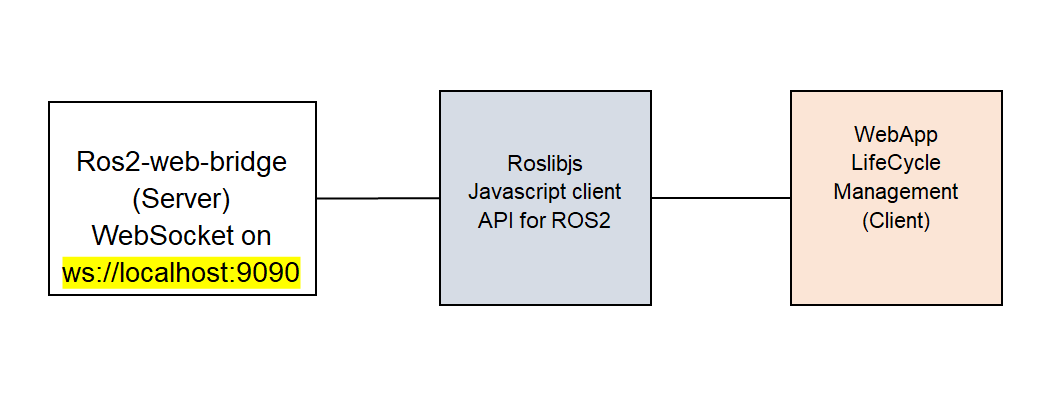
\includegraphics[width=0.95\textwidth]{"Bilder/webapp-design.png"}
		\caption{Overview of Lifecycle Management WebApp}
		\label{fig:Background:WebappDesign}					
	\end{figure}

\subsection{ROS2 Message Types/ JavaScript Objects}
This section describes the ROS2 Messages and Services used to communicate with the ROS2 backend application. There was also a need to explore and examine various JavaScript counterparts to these message and service types. Messages and services  used in the developed application are listed below with their definitions. 

\paragraph{Messages:} 
\begin{itemize}
	\item \lstinline{lifecycle_msgs/msg/State}
\begin{lstlisting}[language=msg,
	caption={Message definition State}]
	# State definitions
	uint8 PRIMARY_STATE_UNKNOWN = 0
	uint8 PRIMARY_STATE_UNCONFIGURED = 1
	uint8 PRIMARY_STATE_INACTIVE = 2
	uint8 PRIMARY_STATE_ACTIVE = 3
	uint8 PRIMARY_STATE_FINALIZED = 4

	uint8 TRANSITION_STATE_CONFIGURING = 10
	uint8 TRANSITION_STATE_CLEANINGUP = 11
	uint8 TRANSITION_STATE_SHUTTINGDOWN = 12
	uint8 TRANSITION_STATE_ACTIVATING = 13
	uint8 TRANSITION_STATE_DEACTIVATING = 14
	uint8 TRANSITION_STATE_ERRORPROCESSING = 15

	## Fields

	# The state id value from the above definitions.
	uint8 id
	# A text label of the state.
	string label
\end{lstlisting}

\item \lstinline{lifecycle_msgs/msg/Transition}
\begin{lstlisting}[language=msg,
	caption={Message definition Transition}]
	# Transition id definitions
	uint8 TRANSITION_CREATE = 0
	uint8 TRANSITION_CONFIGURE = 1
	uint8 TRANSITION_CLEANUP = 2
	uint8 TRANSITION_ACTIVATE = 3
	uint8 TRANSITION_DEACTIVATE = 4
	uint8 TRANSITION_UNCONFIGURED_SHUTDOWN  = 5
	uint8 TRANSITION_INACTIVE_SHUTDOWN = 6
	uint8 TRANSITION_ACTIVE_SHUTDOWN = 7
	uint8 TRANSITION_DESTROY = 8
	uint8 TRANSITION_ON_CONFIGURE_SUCCESS = 10
	uint8 TRANSITION_ON_CONFIGURE_FAILURE = 11
	uint8 TRANSITION_ON_CONFIGURE_ERROR = 12
	uint8 TRANSITION_ON_CLEANUP_SUCCESS = 20
	uint8 TRANSITION_ON_CLEANUP_FAILURE = 21
	uint8 TRANSITION_ON_CLEANUP_ERROR = 22
	uint8 TRANSITION_ON_ACTIVATE_SUCCESS = 30
	uint8 TRANSITION_ON_ACTIVATE_FAILURE = 31
	uint8 TRANSITION_ON_ACTIVATE_ERROR = 32
	uint8 TRANSITION_ON_DEACTIVATE_SUCCESS = 40
	uint8 TRANSITION_ON_DEACTIVATE_FAILURE = 41
	uint8 TRANSITION_ON_DEACTIVATE_ERROR = 42
	uint8 TRANSITION_ON_SHUTDOWN_SUCCESS = 50
	uint8 TRANSITION_ON_SHUTDOWN_FAILURE = 51
	uint8 TRANSITION_ON_SHUTDOWN_ERROR = 52
	uint8 TRANSITION_ON_ERROR_SUCCESS = 60
	uint8 TRANSITION_ON_ERROR_FAILURE = 61
	uint8 TRANSITION_ON_ERROR_ERROR = 62
	uint8 TRANSITION_CALLBACK_SUCCESS = 97
	uint8 TRANSITION_CALLBACK_FAILURE = 98
	uint8 TRANSITION_CALLBACK_ERROR = 99
	
	## Fields

	# The transition id from above definitions.
	uint8 id
	# A text label of the transition.
	string label
\end{lstlisting}

\item \lstinline{lifecycle_msgs/msg/TransitionDescription}
\begin{lstlisting}[language=msg,
	caption={Message definition TransitionDescription}]
	# The transition id and label of this description.
	Transition transition
	# The current state from which this transition transitions.
	State start_state
	# The desired target state of this transition.
	State goal_state
\end{lstlisting}

\item \lstinline{lifecycle_msgs/msg/TransitionEvent}
\begin{lstlisting}[language=msg,
	caption={Message definition TransitionEvent}]
	# The time point at which this event occurred.
	uint64 timestamp
	# The id and label of this transition event.
	Transition transition
	# The starting state from which this event transitioned.
	State start_state
	# The end state of this transition event.
	State goal_state
\end{lstlisting}

\item \lstinline{rcl_interfaces/msg/Log}
\begin{lstlisting}[language=msg,
	label={code:ROS:Message definition Log},
	caption={Message definition Log}]
	##
	## Severity level constants
	## 
	## Since there are several other logging enumeration standard for different implementations,
	## other logging implementations may need to provide level mappings to match their internal implementations.
	##
	# Debug is for pedantic information, which is useful when debugging issues.
	byte DEBUG=10
	# Info is the standard informational level and is used to report expected
	# information.
	byte INFO=20
	# Warning is for information that may potentially cause issues or possibly unexpected
	# behavior.
	byte WARN=30
	# Error is for information that this node cannot resolve.
	byte ERROR=40
	# Information about a impending node shutdown.
	byte FATAL=50
	## Fields

	# Timestamp when this message was generated by the node.
	builtin_interfaces/Time stamp
	# Corresponding log level, see above definitions.
	uint8 level
	# The name representing the logger this message came from.
	string name
	# The full log message.
	string msg
	# The file the message came from.
	string file
	# The function the message came from.
	string function
	# The line in the file the message came from.
	uint32 line
\end{lstlisting}

\end{itemize}

\paragraph{Services:}

\begin{itemize}
	\item \lstinline{lifecycle_msgs/srv/ChangeState}
A ROS2 Service has the following structure:
\begin{lstlisting}[language=service,
	caption={Service definition ChangeState},
	label={code:ROS:Service definition ChangeState}]
	# The requested transition.
	Transition transition
	---
	# Indicates whether the state transition was successful
	bool success
\end{lstlisting}



\item \lstinline{lifecycle_msgs/srv/GetAvailableStates}
\begin{lstlisting}[language=service,
	caption={Service definition GetAvailableStates},
	label={code:ROS:Service definition GetAvailableStates}]
	---
	# Array of possible states that can be transitioned to.
	State[] available_states
\end{lstlisting}

\item \lstinline{lifecycle_msgs/srv/GetAvailableTransitions}
\begin{lstlisting}[language=service,
	caption={Service definition GetAvailableTransitions},
	label={code:ROS:Service definition GetAvailableTransitions}]
	---
	# An array of the possible start_state-goal_state transitions
	TransitionDescription[] available_transitions

\end{lstlisting}

\item \lstinline{lifecycle_msgs/srv/GetState}
\begin{lstlisting}[language=service,
	caption={Service definition GetState},
	label={code:ROS:Service definition GetState}]
	---
	# The current state-machine state of the node.
	State current_state
\end{lstlisting}

\end{itemize}



ROSLIB.ServiceRequest
ROSLIB.Service
ROSLIB.Topic


\paragraph{JavaScript Objects}
\begin{itemize}

\item ROSLIB.Service
\begin{lstlisting}[language=JavaScript,
	label={JavsScript:ROSLIB.Service}
	caption={JavaScript object definition for Service}]
	{
		ros : this.ros,
		name : `/lifecycle_node/get_state`,
		serviceType : 'lifecycle_msgs/GetState'
	}
\end{lstlisting}

\item ROSLIB.ServiceRequest
\begin{lstlisting}[language=JavaScript,
	caption={JavaScript object definition for ServiceRequest}]
	{
		requestParam1 : {requestObject1},
		requestParam2 : {requestObject2},
		...
    }
	}
\end{lstlisting}


\item ROSLIB.Topic
\begin{lstlisting}[language=JavaScript,
	caption={JavaScript object definition for Topic}]
	{
		ros : this.ros,
		name : '/rosout',
		messageType : 'rcl_interfaces/msg/Log'
	}
\end{lstlisting}
\end{itemize}

\paragraph{JSON Objects} A JavaScript application uses JSON Objects to communicate over a network. A JSON object is returned when a ROS service is called or a topic is subscribed to. It is necessary to parse and process these objects to display or update information on a web page. To parse a JSON object, prior knowledge of its structure is required. \\

 \textit{JSON (JavaScript Object Notation) is a lightweight format for data exchange. Working with it is easy for humans likewise machines. It is based on a subset of the JavaScript Programming Language Standard ECMA-262 3rd Edition - December 1999. JSON is a text format that does not depend on any specific language but uses conventions familiar to the C language family, including} \lstinline{C, C++, C#, Java, JavaScript, Perl, Python}, \textit{and many others. These properties make JSON an ideal language for data exchange.}\cite{jsonDef} \\

 In the following section JSON objects used by the developed application is described in detail.
\begin{itemize}
\item  \lstinline{current_state}
\begin{lstlisting}[language=json,
	label={code:ROS:JSON state},
	caption={JavaScript object definition for \lstinline{state}}]
	{
		"current_state": {
			"id": 1,
			"label": "unconfigured"
		}
	}
\end{lstlisting}
\newpage
\item \lstinline{transition}
\begin{lstlisting}[language=json,
	label={code:ROS:JSON transitoin},
	caption={JavaScript object definition \lstinline{transition}}]
	{
		"transition": {
			"id": 1,
			"label": "configure"
		},
		"start_state": {
			"id": 1,
			"label": "unconfigured"
		},
		"goal_state": {
			"id": 10,
			"label": "configuring"
		}
	}
\end{lstlisting}

\item \lstinline{available_transitions}
\begin{lstlisting}[language=json,
	label={code:ROS:JSON available transitions},
	caption={JavaScript object definition for \lstinline{available_transitions}}]
	{
		"available_transitions": [
		  {
			"transition": {
			  "id": 1,
			  "label": "configure"
			},
			"start_state": {
			  "id": 1,
			  "label": "unconfigured"
			},
			"goal_state": {
			  "id": 10,
			  "label": "configuring"
			}
		  },
		  {
			"transition": {
			  "id": 5,
			  "label": "shutdown"
			},
			"start_state": {
			  "id": 1,
			  "label": "unconfigured"
			},
			"goal_state": {
			  "id": 12,
			  "label": "shuttingdown"
			}
		  }
		]
	  }
\end{lstlisting}



\item \lstinline{available_states}
\begin{lstlisting}[language=json,
	label={code:ROS:JSON available states},
	caption={JavaScript object definition \lstinline{available_states}}]
	{
		"available_states": [
			{
			"id": 0,
			"label": "unknown"
			},
			{
			"id": 1,
			"label": "unconfigured"
			},
			...
		]
	}
\end{lstlisting}

\end{itemize}


\subsection{Code Overview} For developing the web application a web framework called VueJS (described in section \ref{Grundlagen:Vue}) is used. This allows the use of various pre-built html components and streamlined application structure with various plugins which in turn makes the UI development structured and easier. The UI part is encapsulated inside the template tag and the JavaScript part in the script tag of a Vue component(described in section \ref{Vue:Component}). The project structure described in \ref{sec:StructureofVue.jsProject} is used.   
\\

To secure a connection to the ROS2 backend through RosLibJS a ROSLIB.Ros Object needs to be initialized and assigned to a variable that can be accessed by all other functions in the application. This object consists of a URL parameter, which will be used to assign the URL of the WebSocket. The WebSocket is made available by the library ros2-web-bridge. This is our main instance of RosLibJS and the same instance will be used throughout the application for working with a single Lifecycle Node. In the case where multiple lifecycle nodes are added, multiple instances of RosLibJS are created and stored. The details of the JavaScript part of the application is described below:

\paragraph{Library imports} The libraries are imported using the standard ES6 syntax. The libraries including Vue-plugins to be installed are listed in the package.json file. This import syntax allows the import of the entire library or only specific components of the library. The following libraries are used:

\begin{lstlisting}[language=JavaScript,
	% caption={dockerfile_startup}, 
	label={code:Vue}]
	import * as ROSLIB from 'roslib';
	import { MDBBtn, MDBBtnGroup, MDBInput, MDBContainer, MDBRow, MDBCol } from "mdb-vue-ui-kit";
\end{lstlisting}

\paragraph{Vue Component initialization} To be able to use the imported components in the HTML-Layout they need to be initialized. The components to be used must be included within the component directive. Also the name of the component is assigned, this name will be used to import this component into any other component. 
\begin{lstlisting}[language=JavaScript,
	% caption={dockerfile_startup}, 
	label={code:Vue}]
	export default {
	
		name: 'LifecycleManagement',
		components: {
			MDBBtn, MDBBtnGroup, MDBInput, MDBContainer, MDBRow, MDBCol
		},
		....
	}
\end{lstlisting}

\paragraph{Declaring global variables} The data directive represents a storage of the necessary attributes for the component. All the global variables are declared in here.The original data object can be accessed with \texttt{\textcolor{purple}{this.data}} directive anywhere inside the component.
\begin{lstlisting}[language=JavaScript,
	% caption={dockerfile_startup}, 
	label={code:Vue}]
	data: function () {
		return {
			unsub: false,
			console_out: [],
			selected_logger_level: 20,
			input_node_name:"",
			added_nodes:["lifecycle_joytovel"],
			active_node: "lifecycle_joytovel",
			selected_transition: {},
			available_states: [],
			available_transitions: [],
			current_state: {},
			ros: new ROSLIB.Ros({
				url : 'ws://localhost:9090'
			})
		}
	},
\end{lstlisting}

\paragraph{Method definitions} All the functions and methods necessary for the application are to be defined inside the methods directive. All the methods used in this application are described in the section \ref{Implementation:ImportantFunctions}.
\begin{lstlisting}[language=JavaScript,
	% caption={dockerfile_startup}, 
	label={code:Vue}]
	methods: {
		...
	},
\end{lstlisting}

\newpage
\paragraph{Vue instance lifecycle hook (mounted)} A Vue component has several lifecycle hooks (described in section \ref{Vue:Instancelifecyclehooks}), which lets a developer customize its behavior at any specific point in its lifecycle. In this application the mounted hook is used to establish a connection to the WebSocket created by the ROS2-Web-Bridge.
\begin{lstlisting}[language=JavaScript,
	% caption={dockerfile_startup}, 
	label={code:Vue}]
	mounted: function () {
		var ros = new ROSLIB.Ros({
			url : 'ws://localhost:9090'
		});

		ros.on('connection', function() {
			console.log('Connected to websocket server.');
		});

		ros.on('error', function(error) {
			console.log('Error connecting to websocket server: ', error);
		});

		ros.on('close', function() {
			console.log('Connection to websocket server closed.');
		});

		this.update();
	},
\end{lstlisting}

\subsection{Important Functions/Methods}
\label{Implementation:ImportantFunctions}
Using RosLibJS the frontend application can be connected to the backend API(websocket) provided by ROS2-web-bridge. To get the required information about the ROS2 nodes running inside the backend application several ROS2 services need to called and some ROS2 topics need to be subscribed to. The methods used to realize these functionalities are described below in detail. These methods are all included inside the \textit{methods} directive described in previous section. As described in listing \ref{{JavsScript:ROSLIB.Service} caption} a ROSLIB.Service object needs to be created every time a service needs to be called. It has a name parameter which has the 
following syntax: 
\begin{lstlisting}
	name: '/<name of the active node>/<name of the service>'
\end{lstlisting}
This convention is utilized in all the following methods in this section.

\paragraph{Methods to add lifecycle nodes and activate it} The \lstinline{add_node} method takes in the name of the lifecycle node provided through the UI and appends it to an array. Multiple lifecycle nodes can be added to the application using this method. To activate a node the \lstinline{set_active_node} method is called. This selects a node from an array of nodes and sets it as the active node. It also clears all the fields in the UI and updates it based on the data received for the active node. The methods for clearing and updating the UI are described in listing \ref{Implementation:Auxillary functions}.
\begin{lstlisting}[language=JavaScript,
	% caption={dockerfile_startup}, 
	label={code:Vue}]
	add_node(){
	  if (this.input_node_name !== "") {
		this.added_nodes.push(this.input_node_name);
		console.log(this.added_nodes);
	  } 
	},

	set_active_node(data){
		this.active_node = data;
		this.clear();
		this.update();
	},
\end{lstlisting}


\paragraph{Service to get CurrentState} This method calls a ROS service to get the current state of the active lifecycle node. A new service object is created, as parameters, the global RosLibJS instance, the complete name of the service, and the service type is passed. All the available services for a lifecycle node are listed in listing \ref{code:ROS2:AvailableServices}. According to the service definition in listing \ref{code:ROS:Service definition GetState}, a ROSLIB.ServiceRequest object is created. This ServiceRequest object is then passed as a parameter to the callService function of the Service object created in the previous step.
The callService function takes three parameters:
\begin{lstlisting}
    serviceObject.callService(request, <result_handler>, <error_handler>)
\end{lstlisting}
The first parameter is the ServiceRequest object, second and third are JavaScript Arrow Functions to extract the result of the service and error message. The third parameter is optional. The structure of the result object is described in listing \ref{code:ROS:JSON state}. The current state is extracted from the result object and the global currentState variable is updated.
\begin{lstlisting}[language=JavaScript,
	% caption={dockerfile_startup}, 
	label={code:Vue}]
	srvGetCurrentState() {
		var lifecycleClient = new ROSLIB.Service({
			ros : this.ros,
			name : `/${this.active_node}/get_state`,
			serviceType : 'lifecycle_msgs/GetState'
		});

		var request = new ROSLIB.ServiceRequest({});

		lifecycleClient.callService(request, 
			(result) => {
				console.log(result);
				this.current_state = result.current_state;
			}
		)
		
		},
\end{lstlisting}

\paragraph{Service to get all available States} This method calls a ROS service to get the all available states of the active lifecycle node. A new service object is created, similar to the last example. According to the service definition in listing \ref{code:ROS:Service definition GetAvailableStates}, a ROSLIB.ServiceRequest object is created. The structure of the result object is described in listing \ref{code:ROS:JSON available states}. All available states are extracted from the result object, stored in a temporary array and the global availableStates array is updated.
\begin{lstlisting}[language=JavaScript,
	caption={Method to get available States}, 
	label={code:Vue}]
	srvGetAvailableStates() {
	  var lifecycleClient = new ROSLIB.Service({
		ros : this.ros,
		name : `/${this.active_node}/get_available_states`,
		serviceType : 'lifecycle_msgs/GetAvailableStates'
	  });

		var request = new ROSLIB.ServiceRequest({});
		var tempArr = [];

		lifecycleClient.callService(request, 
		  (result) => {
			console.log(result);
			result.available_states.forEach(element => {
				console.log(element);
				tempArr.push(element);
			});
			this.available_states = tempArr;
		})
	},

\end{lstlisting}

\paragraph{Service to get AvailableTransitions} This method calls a ROS service to get all available transitions of the active lifecycle node. A new service object is created, similar to the last example. According to the service definition in listing \ref{code:ROS:Service definition GetAvailableTransitions}, a ROSLIB.ServiceRequest object is created. The structure of the result object is described in listing \ref{code:ROS:JSON available transitions}. All available transitions are extracted from the result object, stored in a temporary array and the global availableTransitions array is updated.
\begin{lstlisting}[language=JavaScript,
	caption={Method to get available Transitions}, 
	label={code:Vue}]
	srvGetAvailableTransitions() {
	  var lifecycleClient = new ROSLIB.Service({
		ros : this.ros,
		name : `/${this.active_node}/get_available_transitions`,
		serviceType : 'lifecycle_msgs/GetAvailableTransitions'
	  });

	  var request = new ROSLIB.ServiceRequest({});
	  var tempArr = [];
	
	  lifecycleClient.callService(request, 
		(result) => {
		result.available_transitions.forEach(
			element => {
			tempArr.push(element);
		});
		this.available_transitions = tempArr;
	  })
	},
\end{lstlisting}


\paragraph{Service to ChangeState} This method calls a ROS service to change the current state of the active lifecycle node to any valid state. A new service object is created, similar to the last example. According to the service definition in listing \ref{code:ROS:Service definition ChangeState}, a ROSLIB.ServiceRequest object is created. The ServiceRequest object requires a transition parameter, which consist a transition ID and a label. Transition ID can be selected in the UI, the available selections in UI is determined by a automatic state transition logic. The result in this case is a Boolean, which indicates if the transition was successful. Then the update method is called.
\begin{lstlisting}[language=JavaScript,
	% caption={dockerfile_startup}, 
	label={code:Vue}]
	srvChangeState() {
		var lifecycleClient = new ROSLIB.Service({
			ros : this.ros,
			name : `/${this.active_node}/change_state`,
			// name : '/lifecycle_joytovel/change_state', 
			serviceType : 'lifecycle_msgs/ChangeState'
		});
	
		var r_id = parseInt(this.selected_transition);

		var request = new ROSLIB.ServiceRequest({
			transition: {id: r_id, label : ""}
		});

		lifecycleClient.callService(request, function(result) {
			console.log(result);
		}, function(error) {
			console.log(error);
		});
		this.update();
	},
\end{lstlisting}

\paragraph{Subscribe to rosout} This method is necessary to implement the logging functionality in the UI. A ROSLIB.Topic object is created, which is used to subscribe to ROS topic \lstinline{\rosout}. The relevant log messages for the active lifecycle node is filtered and stored in a rolling array of a fixed size. This array is used by the logger component to display log messages in the UI. Structure of the log message is described in listing \ref{code:ROS:Message definition Log}. The desired log level (DEBUG, INFO, WARN, ERROR or FATAL) can be selected using the mapLogLevel method in listing \ref{Implementation:Auxillary functions}. Using a global unsubscribe flag, the logging can be deactivated from the UI. 
\begin{lstlisting}[language=JavaScript,
	% caption={dockerfile_startup}, 
	label={code:Vue}]
	subscribeToRosOut(){
		var listener = new ROSLIB.Topic({
			ros : this.ros,
			name : '/rosout',
			messageType : 'rcl_interfaces/msg/Log'
			});

			var msg = [];
			listener.subscribe((msg)=> {
				this.console_out.push(msg);
				if (this.console_out.length > 10) {
					this.console_out.shift();
				}
				
				if (this.unsub) {
					listener.unsubscribe();
				}
			}) 
			console.log(msg);
		},
\end{lstlisting}

\paragraph{Auxiliary Methods/Functions} These are some auxiliary methods/functions used in this Vue component.
\label{Implementation:Auxillary functions}
\begin{lstlisting}[language=JavaScript,
	caption={Auxillary functions}, 
	label={code:Auxillary functions}]
	clear() {
		this.available_states = [];
		this.current_state = [];
		this.available_transitions = [];
	},

	update() {
		this.srvGetCurrentState()
		this.srvGetAvailableTransitions()
		this.srvGetAvailableStates()
	},

	mapLogLevel(level){
		if (level === 10) {
			return "DEBUG"
		} 
		else if (level === 20){
			return "INFO"
		}
		else if (level === 30){
			return "WARN"
		}
		else if (level === 40){
			return "ERROR"
		}
		else if (level === 10){
			return "FATAL"
		}
	}
\end{lstlisting}
% \begin{lstlisting}[language=JavaScript,
% 		% caption={dockerfile_startup}, 
% 		label={code:Vue}]
		
% 	methods: {
% 		// Available Services :
% 		// /lifecycle_joytovel/change_state
% 		// /lifecycle_joytovel/describe_parameters
% 		// /lifecycle_joytovel/get_available_states
% 		// /lifecycle_joytovel/get_available_transitions
% 		// /lifecycle_joytovel/get_parameter_types
% 		// /lifecycle_joytovel/get_parameters
% 		// /lifecycle_joytovel/get_state
% 		// /lifecycle_joytovel/get_transition_graph
% 		// /lifecycle_joytovel/list_parameters
% 		// /lifecycle_joytovel/set_parameters
% 		// /lifecycle_joytovel/set_parameters_atomically
% \end{lstlisting}

\subsection{Lifecycle Dashboard UI}
The developed user interface is depicted in the figure \ref{fig:Implementation:LifecycleDashboard}. 
The functionalities of the web interface is based on the Lifecycle Management CLI described in section \ref{Lifecycle management CLI}. At the top of the UI there is a text-field that takes the name of the lifecycle node as an input. The button adjacent to it can be pressed in order to add the desired node to the list of added nodes. It is possible to add multiple nodes to the list using this UI component.
The next UI component is a list of buttons with names of the nodes added to the dashboard. A single node can be selected by pressing the desired button to activate the node. The activated node is shown in the next line along with its current state. The following line consists of a list of buttons to call various functions mentioned in section \ref*{Implementation:ImportantFunctions}.
\\

The next line consists of buttons to enable the console logger and enable state transition. For state transition there is a dropdown list consisting of valid states to be transition to. From this list the desired transition state can be selected and the state transition button next to it can be pressed to execute the desired transition. Below is table with the detail description of the available state transitions. 
\\

There is also a list of all available states for the active lifecycle node. Next to it is a console logger which constantly displays the application logs of the currently running lifecycle node. On top of the logger UI component there is a dropdown menu consisting of different available log levels. The log levels are listed in the listing \ref{code:Auxillary functions} Upon selection of desired log level only the corresponding logs are displayed. At the very bottom of the page there is a button to disable the logger for the active node.
\\

When a new lifecycle node is added to the dashboard or selected, the entire UI resets to the initial condition and the logs are cleared.

\vspace{5cm}
\begin{figure}[H]
	\centering
	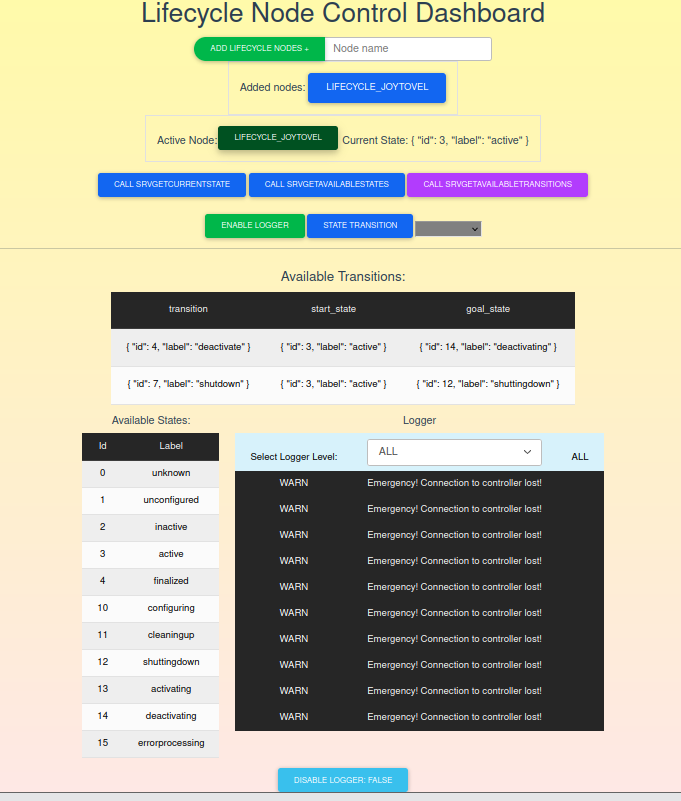
\includegraphics[width=0.99\textwidth]{"Bilder/lifecycle-dashboard.png"}
	\caption{Lifecycle Dashboard}
	\label{fig:Implementation:LifecycleDashboard}					
\end{figure}

\newpage
\vspace*{1cm}
\section{Integration}
\label{Implementierung:Integration}
The developed application consists of different software components from several different open source organizations and Siemens. These components use different programming languages and it is necessary to connect them using the required interfaces. They must all work together to have a properly functioning application. To run the complete application several software components need to be started in the correct order depending on their interdependency. First of all the native ROS2 application is built and started, then the ros2-web-bridge interface is started, and finally, a web application(Lifecycle management interface) is built and a web server(nginx) is started to run the Lifecycle Management Interface. The application is containerized as described in section \ref{Implementierung:DockerEnvironment}, and most of the integration and cross-communication between the components is achieved within the aforementioned Dockerfile. 
\\ 

Furthermore, the application needs to be integrated into the Siemens Industrial Edge ecosystem, which is described in the following section.
\vspace{1cm}
\subsection{Conversion to Industrial Edge Application} 
The Industrial Edge Publisher can be used to convert a docker image into an Industrial Edge Application. The created docker-compose.yml file (listing \ref{Implementation:dockerCompose}) is first imported into the Industrial Edge Publisher. The created images along with their various configurations are recognized by the Industrial Edge environment and these configurations are automatically applied when the application is installed on the Edge Device. No further configuration is necessary for the Edge App. Once the application has been created, it can be uploaded to the IEM using the Industrial Edge Publisher, where it is available for further distribution.

\paragraph{Docker Compose File}
With a docker-compose.yml file, services and configurations can be specified for a Docker container. This application requires several Docker containers to communicate with each other, for this purpose a separate network is created in the docker-compose file. In addition, a volume is created to store any persistent data that might be useful for the application.
\\


In the services section of the docker-compose file, the Docker image in the current directory is built. The name of the created Docker image is then specified. Then with the start command a \gls{ROS2} Application with lifecycle node is run. The commands \lstinline{mem_limit: 500mb} and \lstinline{restart: on-failure} are necessary for Industrial Edge. Then the docker volume created in the previous step is mounted. The network to use is specified then the docker container is connected to the network.
\vspace*{2cm}
\begin{lstlisting}[language=docker-compose,
		caption={docker-compose.yaml used by IE Publisher},
		label={Implementation:dockerCompose}]
		networks :
 			ie-app-network :
	 			name : ie-app-network

		volumes:
			lifecycle_edge:
				name: lifecycle_edge
		
		services:
			ros2-lifecycle:
				build: ./
				image: ros2_foxy_lifecycle:1.0
				command: ros2 launch evo_siemensrob_ctrl agv_control_launch.py 
				mem_limit: 500mb
				restart: on-failure
				volumes:
					- lifecycle_edge
				networks:
					- ie-app-network		
\end{lstlisting}
	
The complete source code of this application is available on GitHub under following link: \url{https://github.com/dspwithaheart/ROS2Lifecycle.git}
	
	% \chapter{Proof of Concept}
\label{PoC}

	\section{Manueller Test}
	\label{Design:Struktur}
		- Prozess soll von Laien ausführbar sein
	
	\section{Integration in Edge}
	\label{Design:Abhängigkeiten}
	
	\section{Fusionierung mehrerer Projekte}
	\label{PoC:Fusionierung}	
	
	\chapter{Discussion}
\label{Discussion}

Introduction of ROS2 Applications with managed lifecycle alone provides huge improvement to the overall operation of a mobile robot system. It provides the potential for reducing operational and maintenance costs and improves the compatibility of an application with other future applications. A ROS2 Application with managed lifecycle opens up several potential use cases and advantages during the operation of a mobile robot.
\\

It enables dynamic reconfiguration of various operating parameters of component nodes (applications) within a robot system. Configurations for different hardware sensors and actuators of a robot can be adjusted remotely and individually just by switching the state of an application (node). Other applications (node) can continue performing their designated functions while others are being reconfigured depending on the current conditions. For example, the input sensitivity of a joystick can be changed or a damaged modular component (camera, laser scanner, etc.) can be changed and reconfigured while the rest of the system keeps running. It also allows respawning or restarting of any independent subsystem on the fly. If a sub-application (node) depends on another sub-application (node) it can switch to an idle state and wait for another application to be fully functional without shutting itself down completely. This localizes any failure to a sub-application which can then be diagnosed and repaired individually. This also enables active status monitoring of various subsystems for early and efficient maintenance. Managed lifecycle also improves the error logging process of various subsystem applications. This in turn streamlines the debugging process by providing a detailed and more descriptive remote logging system. This adds a level of efficiency to the system and makes the overall operation smoother. It also lays the foundation for achieving complete modularity.
\\

The objective of modern Application Development is for many developers to work simultaneously on different functions of the same application. If an organization is set up so that all functionalities are to be merged in a single instance, the consequential work can be tedious, manual, and time-consuming. When a developer working in isolation makes a change to an application, it may conflict with other changes made simultaneously by other developers. This problem is compounded if each developer has customized their local development environment. One of the objectives of this thesis is to improve the overall stability and compatibility of the applications developed by the organization. Which includes the improvement and refinement of the development and operational environment of the developed applications. To achieve complete automation in the software integration and deployment of ROS2-based mobile robots steps relating to building a CI/CD pipeline are necessary. 
\\

\textit{
CI/CD is a method for deploying applications continually to end users by introducing automation into the application development stages. The core concepts associated with CI/CD are continuous integration, continuous delivery, and continuous deployment. CI/CD provides a solution to the challenges posed to development and operational teams through the integration of new code. In particular, it introduces end-to-end automation and constant monitoring during the entire application lifecycle, from the integration and testing phase through to the deployment phase.\cite*{cicdOverwiew}}
\\

This is achieved by containerizing the ROS2 Applications in Docker containers, which are then converted to IE Apps that can be uploaded to IE Hub for further deployment. Above mentioned design and implementation provide the following advantages:


\begin{itemize}
	\item 	Allows package updates to be installed without shutting down the entire system. (Modularity/ CI/CD)
	\item 	Streamlines the debugging and error logging process of subsystem applications.
	\item 	Simplifies the installation of additional modular components on an existing mobile robot or the sharing of modular components among a group of robots.
	\item 	Enables active status monitoring of various subsystems for early and efficient maintenance.
	\item 	Prevents total system failure by loosely coupling different subsystems and avoiding a monolithic architecture.
	\item 	Provides developers with the freedom to choose from different libraries and frameworks which do not have to be version compatible.
	\item 	Supports the development of an autonomously operating and updating fleet of mobile robots.
\end{itemize}

\chapter{Conclusion and Future Work}
\label{: Conclusion and Future Work}
	This thesis demonstrates the development process of a ROS2 based Robot Applications with inbuilt Lifecycle. Furthermore the application is packed into a Docker environment which further simplifies the development process and helps integrate custom ROS2 applications into an existing Siemens Industrial Edge ecosystem. The developed Lifecycle Management Interface serves as a prototype for further development. An agile and modern web framework (VueJS) was used to develop the above mentioned Lifecycle Management Interface which allows for efficient addition of further functionalities to it.  
    \\
	
    The developed Lifecycle Management Interface will help and improve the overall stability of various mobile Robots developed using ROS2. It will further facilitate integration of the newly developed mobile robots into an existing ecosystem. It will also ensure cross compatibility of mobile robots and enable development of application in field of swarm robotics. The potential use cases of this Lifecycle Management Application will be discussed in the following chapter in detail.
    \\

    Another major part of this thesis is the Dockerisation of ROS2 based Applications. It provides major advantages in the development, deployment and operational cycle of a mobile robot. It is a step towards developing a CI/CD pipeline for the mobile robot development. With integration of Docker into the system, there is no need to develop a Operating System specific ROS Applications. With Docker multiple Applications with different Operating Systems and OS versions can run seamlessly on a single Computer system. It introduces a concept of microservices from web development into the ROS world. Which further simplifies the Network configuration and communication stability. A dockerized ROS2 application is then converted into Siemens Industrial Edge App. There is an existing ecosystem of IE Apps with an Appstore. After the conversion the ROS2 IE Apps can be downloaded from the IE Appstore and installed on a mobile robot without much hassle. 
    \\
    
    The Web interface for LifecycleManagement allows addition of multiple ROS2 nodes to the dashboard to be tracked and controlled. For a selected node the dashboard shows the current state of the node, available transitions and relevant log output to the console. From the dashboard it is possible to change the state of a lifecycle node to any other viable state. The automatic state transition has been implemented in the dashboard which only shows valid transitions.
    \\

    The development of ROS2-based IE Apps is still in the research and development phase and there is a lot of room for improvement. The frameworks and design patterns used for the developed application support further extension and improvement. Which should ensure compatibility with other applications developed in the future by the organization. The level of automation in the development process of the ROS2 Application is improved. Above all the viability, development process, and advantages of developing a ROS2 application with a managed lifecycle in a Docker environment are described in this thesis. 	
	
	
	
	
	\label{Ende} % Wichtig für Fußnote "Seite X von Y"	
	\clearpage
			
	% Für Anhang wieder umstellen auf Römische Seitenzähler

	\pagenumbering{Roman}
	\setcounter{page}{\value{SeitenzahlSpeicher}}
	\ofoot{\pagemark}
	
	% Literaturverzeichnis
	\printbibliography[title={References}]
	
	% Abbildungsverzeichnis
	\listoffigures 
	
	% Tabellenverzeichnis
	\listoftables
	
	% Listing-Verzeichnis
	% Namen definieren
	% \renewcommand{\lstlistlistingname}{Verzeichnis der Listings}
	\lstlistoflistings
	
	
\end{document}